%---------------------------------------------------------------------------%
%-                                                                         -%
%-                           LaTeX Template                                -%
%-                                                                         -%
%---------------------------------------------------------------------------%
%- Copyright (C) Huangrui Mo <huangrui.mo@gmail.com> 
%- This is free software: you can redistribute it and/or modify it
%- under the terms of the GNU General Public License as published by
%- the Free Software Foundation, either version 3 of the License, or
%- (at your option) any later version.
%---------------------------------------------------------------------------%
%->> Document class declaration
%---------------------------------------------------------------------------%
\documentclass[twoside]{Style/ucasthesis}%
%- Multiple optional arguments:
%- [<oneside|twoside|print>]% oneside eprint, twoside eprint, or paper print
%- [fontset=<adobe|none|...>]% specify font set instead of automatic detection
%- [scheme=plain]% thesis writing of international students
%- [draftversion]% show draft version information
%- [standard options for ctex book class: draft|paper size|font size|...]%
%---------------------------------------------------------------------------%
%->> Document settings
%---------------------------------------------------------------------------%
\usepackage[super,list,math,geometry,color]{Style/artratex}% document settings
%- usage: \usepackage[option1,option2,...,optionN]{artratex}
%- Multiple optional arguments:
%- [bibtex|biber]% set bibliography processor and package
%- [<numbers|super|authoryear|alpha>]% set citation and reference style
%- <numbers>: textual: Jones [1]; parenthetical: [1]
%- <super>: textual: Jones superscript [1]; parenthetical: superscript [1]
%- <authoryear>: textual: Jones (1995); parenthetical: (Jones, 1995)
%- <alpha>: textual: not available; parenthetical: [Jon95]
%- [geometry]% reconfigure page layout via geometry package
%- [lscape]% provide landscape layout environment
%- [xhf]% disable header and footer via fancyhdr package
%- [color]% provide color support via xcolor package
%- [background]% enable page background
%- [tikz]% provide complex diagrams via tikz package
%- [table]% provide complex tables via ctable package
%- [list]% provide enhanced list environments for algorithm and coding
%- [math]% enable some extra math packages
%- [xlink]% disable link colors
% user defined commands
\usepackage{Style/artracom}
\usepackage{booktabs}
\usepackage{multirow}
\usepackage{xcolor}
\usepackage{lscape}
\usepackage{stmaryrd,scalerel}
\usepackage[final]{pdfpages}
%---------------------------------------------------------------------------%
%->> Document inclusion
%---------------------------------------------------------------------------%
%\includeonly{Tex/Chap_1,...,Tex/Chap_N}% selected files compilation
%---------------------------------------------------------------------------%
%->> Document content
%---------------------------------------------------------------------------%
%-
%-> Titlepage information
%-
%---------------------------------------------------------------------------%
%->> Titlepage information
%---------------------------------------------------------------------------%
%-
%-> 中文封面信息
%-
\confidential{公开}% 密级:只有涉密论文才填写
\orderid{19111365}
\schoollogo[scale=.8]{ucas_logo}% 校徽
\title{无人机集群行为分类的一致性预测方法研究}% 论文中文题目
\author{席泽璞}% 论文作者
\advisor{陈洪波~教授~中山大学\\陈小前~研究员~军事科学院}% 指导教师:姓名 专业技术职务 工作单位
%\advisor{指导教师一\\指导教师二\\指导教师三}% 多行指导教师示例
\degree{博士}% 学位:学士、硕士、博士
\degreetype{工学}% 学位类别:理学、工学、工程、医学等
\major{计算机科学与技术}% 二级学科专业名称
\institute{中山大学}% 院系名称
%\institute{中国科学院力学研究所\\流固耦合实验室}% 多行院系名称示例
\date{2023~年~6~月}% 毕业日期:夏季为6月、冬季为12月
%-
%-> 英文封面信息
%-
\TITLE{Research on Conformal Prediction Methods for UAV Swarm Behavior Classification}% 论文英文题目
\AUTHOR{ZEPU XI}% 论文作者
\ADVISOR{Supervisor: Professor Hongbo CHEN \\ Professor Xiaoqian CHEN}% 指导教师
\DEGREE{Doctor}% 学位:Bachelor, Master, Doctor, Postdoctor。封面据英文学位名称自动切换,需确保拼写准确
\DEGREETYPE{Natural Science}% 学位类别:Philosophy, Natural Science, Engineering, Economics, Agriculture 等
\MAJOR{Computer Science}% 二级学科专业名称
\INSTITUTE{Sun Yat-sen University}% 院系名称
\DATE{June, 2023}% 毕业日期:夏季为June、冬季为December
%---------------------------------------------------------------------------%
% 封面
\begin{document}
%-
%-> Frontmatter: title page, abstract, content list, symbol list, preface
%-
\frontmatter% initialize the environment
%---------------------------------------------------------------------------%
%->> Frontmatter
%---------------------------------------------------------------------------%
%-
%-> 生成封面
%-
%\maketitle% 生成中文封面
%\MAKETITLE% 生成英文封面
%-
%-> 作者声明
%-
%\makedeclaration% 生成声明页


\includepdf[pages=-]{Tex/FM.pdf} % 更改封面为特定学校的封面
%-
%-> 中文摘要
%-
\intobmk\chapter*{摘\quad 要}% 显示在书签但不显示在目录
\setcounter{page}{1}% 开始页码
\pagenumbering{Roman}% 页码符号

具有高协同、复杂行为模式的无人机集群技术已经被广泛应用于各种军用和民用任务场景。面向不同目标的任务场景, 无人机集群系统需要按照不同的行为完成集群任务。针对无人机集群行为分类的研究为无人机集群意图推演提供具有重要建设性作用的前期信息支持。通过经验观测数据训练机器学习算法可以实现无人机集群行为分类并预测未知无人机集群行为。现有机器学习算法的输出只能提供单值预测, 忽视预测输出结果的置信程度。同时, 无人机集群行为数据随着时间变化会产生分布漂移问题, 现有机器学习算法忽视对分布漂移展开检测。再者, 目前大多数机器学习算法对训练数据样本需求量较大, 忽略在小样本下开展高精度预测模型的构建。

本文围绕利用机器学习实现无人机集群行为分类问题, 研究为分类算法的输出结果提供可信的不确定度量。针对数据分布随时间发生变化的难题, 本文研究无分布假设情形下开展数据分布漂移检测问题。在此基础上, 提出一种鞅保护分布算法提高机器学习模型的预测性能。面对小样本数据下要求实现无人机集群高精度分类难题, 本文研究使用特权信息范式为无人机集群行为分类提供高精度预测。

首先, 对于无人机集群行为分类研究中现有机器学习算法无法为其预测输出提供有效不确定量化难题, 本文提出采用一致性预测算法框架为利用机器学习算法实现无人机集群行为分类问题提供有效不确定量化。通过将机器学习算法的输出结果校正为有效p-值序列, 结合随机算法理论技术提出一种可建立在学习算法之上的无分布假设的有效不确定量化算法框架。本文提出的方法能够提供两种不确定量化模式, 一方面可以提供置信预测, 另一方面可以实现集合预测。通过无人机集群测试算例验证上述方法的有效性, 并对比分析所提方法的实用性。

其次, 从一致性预测理论出发, 针对无人机集群行为数据的分布随着时间发生变化的特点, 结合鞅理论提出无分布假设的分布漂移检测方法。本文提出的方法能够处理超高维数据的分布漂移检测并且无需任何分布假设。通过三种实际无人机集群行为数据, 验证所提鞅序列方法可以检测数据本身的分布随时间发生变化的问题。

此外, 本文将基于鞅序列的分布漂移检测理论应用于机器学习算法的顶层, 提出鞅保护分布算法。此算法在机器学习算法顶层构建保护带, 通过将随着时间变化的分布信息纳入考量来增强底层算法的学习泛化推广能力。研究结果表明, 本文提出的方法对于大多数机器学习算法都能够明显改善其预测能力。

最后, 针对常规机器学习算法大都需要建立在大样本学习机制上的问题, 结合实际工程应用中无人机集群行为数据稀缺的特点, 提出一种在小样本下实现高精度分类的算法。该算法能够将训练阶段可用但测试阶段不可用的信息(本文称之为特权信息)纳入模型, 使得在小样本下达到高精度预测的目标。研究结果表明, 本文提出的算法能够明显提升算法收敛速度, 使得无人机集群行为分类在小样本下也可以达到较高精度的预测效果。


\keywords{无人机集群系统, 集群行为分类, 一致性预测, 分布漂移检测, 使用特权信息学习}
%-
%-> 英文摘要
%-
\intobmk\chapter*{Abstract}% 显示在书签但不显示在目录

UAV swarm with high collaboration and complex behavior patterns has been widely applied in various military and civilian mission scenarios. UAV swarm system needs to complete different tasks according to different behaviors pattern in complex environment. We can make an effective statistical learning inference problem for recovering UAV swarm behavior pattern based on empirical data with the help of modern machine learning algorithms. However, most machine learning algorithms only output similarity measurement between each sample and there is no confidence measure for prediction of output value for particular new objects. At the same time, a common problem in UAV swarm applications of machine learning is that, soon after a prediction algorithm is trained, the distribution of the data may change, and the prediction algorithm may need to be retrained. Furthermore, most machine learning algorithms have a high demand for training data samples and have a low-precision prediction in small samples.

This thesis provide an effective distributions-free uncertainty quantification framework based on conformal prediction for hedging the prediction output. We also propose a distributions-free martingales framework to test distributions-shift. In particular, for speed up the convergence of learning, it is possible that we can build a new learning paradigm of pattern recognition algorithm based on learning using privileged information paradigm. 

Firstly, we propose Mondrian conformal prediction to provide exact valid error control for UAV swarm behavior classification. We adopt Mondrian conformal prediction methods to provide distributions-free uncertainty quantification. Our methods can be build on the top of any machine learning algorithms and provide exactly valid statistical inference. For the reliable machine learning of UAV swarm behavior pattern recognition with the help of Mondrian conformal prediction, we provide not only simple prediction with corresponding exact valid confidence and credibility measurements, but also exact valid set prediction under any user-specified significance level.

Secondly, we propose distributions-free methods to test distributions-shift under conformal test martingales for UAV swarm behavior datasets. The method proposed in this thesis have an effective distributions-shift detection for high-dimensional data without any distribution assumption. We test the proposed method on  three UAV swarm behavior datasets, it has been proven that the proposed martingale method provide an effective tools for distributions-shift detection.

Furthermore, based on the research of conformal test martingale, we find that it is important information that take into account the original order of UAV swarm behavior dataset. In this thesis, we introduce the martingale protected distribution methods that can be build on the top of any machine learning algorithm to integrated the original order of dataset to improve the performance of machine learning algorithm. 

Finally, we propose a new learning paradigm, called learning using privileged information (LUPI), to speed up the convergence of learning for UAV swarm behavior pattern recognition. It is remarkable that the privileged information that supply holistic description information is only available during the training stage rather than available during the test stage. When we introduce the privileged information for UAV swarm behavior pattern recognition, two experiments shows that the LUPI paradigm established well-performance predictive results.


\KEYWORDS{UAV Swarm Systems, Swarm Behaviors Classification, Conformal Prediction, Distributions-shift Detection, Learning Using Privileged Information}% 英文关键词
%---------------------------------------------------------------------------%
% title page, abstract
{% content list region
\linespread{1.2}% local line space
\intobmk*{\cleardoublepage}{\contentsname}% add link to bookmark
\tableofcontents% content catalog
\intobmk*{\cleardoublepage}{\listfigurename}% add link to bookmark
\listoffigures% figure catalog
\intobmk*{\cleardoublepage}{\listtablename}% add link to bookmark
\listoftables% table catalog
}
\intobmk\chapter*{缩略语说明}% 显示在书签但不显示在目录

%\section*{字符}
%\nomenclatureitem[\textbf{Unit}]{\textbf{Symbol}}{\textbf{Description}}
%\nomenclatureitem[$\Unit{m^{2} \cdot s^{-2} \cdot K^{-1}}$]{$R$}{the gas constant}
%\nomenclatureitem[$\Unit{m^{2} \cdot s^{-2} \cdot K^{-1}}$]{$C_v$}{specific heat capacity at constant volume}
%\nomenclatureitem[$\Unit{m^{2} \cdot s^{-2} \cdot K^{-1}}$]{$C_p$}{specific heat capacity at constant pressure}
%\nomenclatureitem[$\Unit{m^{2} \cdot s^{-2}}$]{$E$}{specific total energy}
%\nomenclatureitem[$\Unit{m^{2} \cdot s^{-2}}$]{$e$}{specific internal energy}
%\nomenclatureitem[$\Unit{m^{2} \cdot s^{-2}}$]{$h_T$}{specific total enthalpy}
%\nomenclatureitem[$\Unit{m^{2} \cdot s^{-2}}$]{$h$}{specific enthalpy}
%\nomenclatureitem[$\Unit{kg \cdot m \cdot s^{-3} \cdot K^{-1}}$]{$k$}{thermal conductivity}
%\nomenclatureitem[$\Unit{kg \cdot m^{-1} \cdot s^{-2}}$]{$S_{ij}$}{deviatoric stress tensor}
%\nomenclatureitem[$\Unit{kg \cdot m^{-1} \cdot s^{-2}}$]{$\tau_{ij}$}{viscous stress tensor}
%\nomenclatureitem[$\Unit{1}$]{$\delta_{ij}$}{Kronecker tensor}
%\nomenclatureitem[$\Unit{1}$]{$I_{ij}$}{identity tensor}
%
%\section*{算子}
%\nomenclatureitem{\textbf{Symbol}}{\textbf{Description}}
%\nomenclatureitem{$\Delta$}{difference}
%\nomenclatureitem{$\nabla$}{gradient operator}
%\nomenclatureitem{$\delta^{\pm}$}{upwind-biased interpolation scheme}
%
\section*{缩写}
\nomenclatureitem{Boosting}{提升算法(Boosting)}
\nomenclatureitem{CP}{一致性预测(Conformal Prediction)}
\nomenclatureitem{DT}{决策树(Decision Trees)}
\nomenclatureitem{ICP}{归纳一致性预测(Inductive Conformal Prediction)}
\nomenclatureitem{LR}{逻辑回归(Logistic Regression)}
\nomenclatureitem{LUPI}{使用特权信息学习(Learning Using Privileged Information)}
\nomenclatureitem{MCP}{蒙德里安一致性预测(Mondrian Conformal Prediction)}
\nomenclatureitem{NB}{朴素贝叶斯(Na\"{i}ve Bayes)}
\nomenclatureitem{NN}{神经网络(Neural Networks)}
\nomenclatureitem{PAC}{概率近似正确(Probably Approximately Correct)}
\nomenclatureitem{RF}{随机森林(Random Forests)}
\nomenclatureitem{SVMs}{支持向量机(Support Vector Machines)}
\nomenclatureitem{TCP}{超越一致性预测(Transductive Conformal Prediction)}
\nomenclatureitem{TCM}{超越置信机(Transductive Confidence Machine)}
\nomenclatureitem{TI}{超越推理(Transductive Inference)}
\nomenclatureitem{USS}{无人机集群系统(UAV Swarm Systems)}
\nomenclatureitem{VC Theory}{VC理论(Vapnik-Chervonenkis Theory)}
%
% symbol list, preface content
%-
%-> Mainmatter
%-
\mainmatter% initialize the environment
%---------------------------------------------------------------------------%
%->> Main content
%---------------------------------------------------------------------------%
\chapter{绪论}
\label{chap:introduction}

\section{研究背景与意义}
无人机集群系统(UAV Swarm Systems, USS)是一种模拟生物飞行系统工作原理而设计的新型仿生系统, 具有快速稳定、意志自适应以及集群涌现的工作优势。 集群的概念最早源自生物学研究, 表征个体间的间接协调机制。 这种协调机制表现为集群中的个体在无需任何集中规划和中心化通信情况下, 依靠个体间简单通信完成复杂群体活动的一种运行机制。 集群系统行为研究源于\citet{Flocks1987}等人提出的分离、聚集和速度一致三个基本规则(简称“Boids三原则”)。 基于Boids三原则, 个体通过相互之间的自主决策和简单信息交互, 经过演化最终使得整个群体在宏观上呈现出具有自组织、协作性和稳定性等整体行为特点。如图\ref{fig:swarm}所示, 经过个体之间的演化, 无人机集群系统可衍生出多种行为模式: 如无人机集群排列(Align)行为, 无人机集群聚集(Flock)行为和无人机集群组队(Group)行为等。

\begin{figure}
\centering
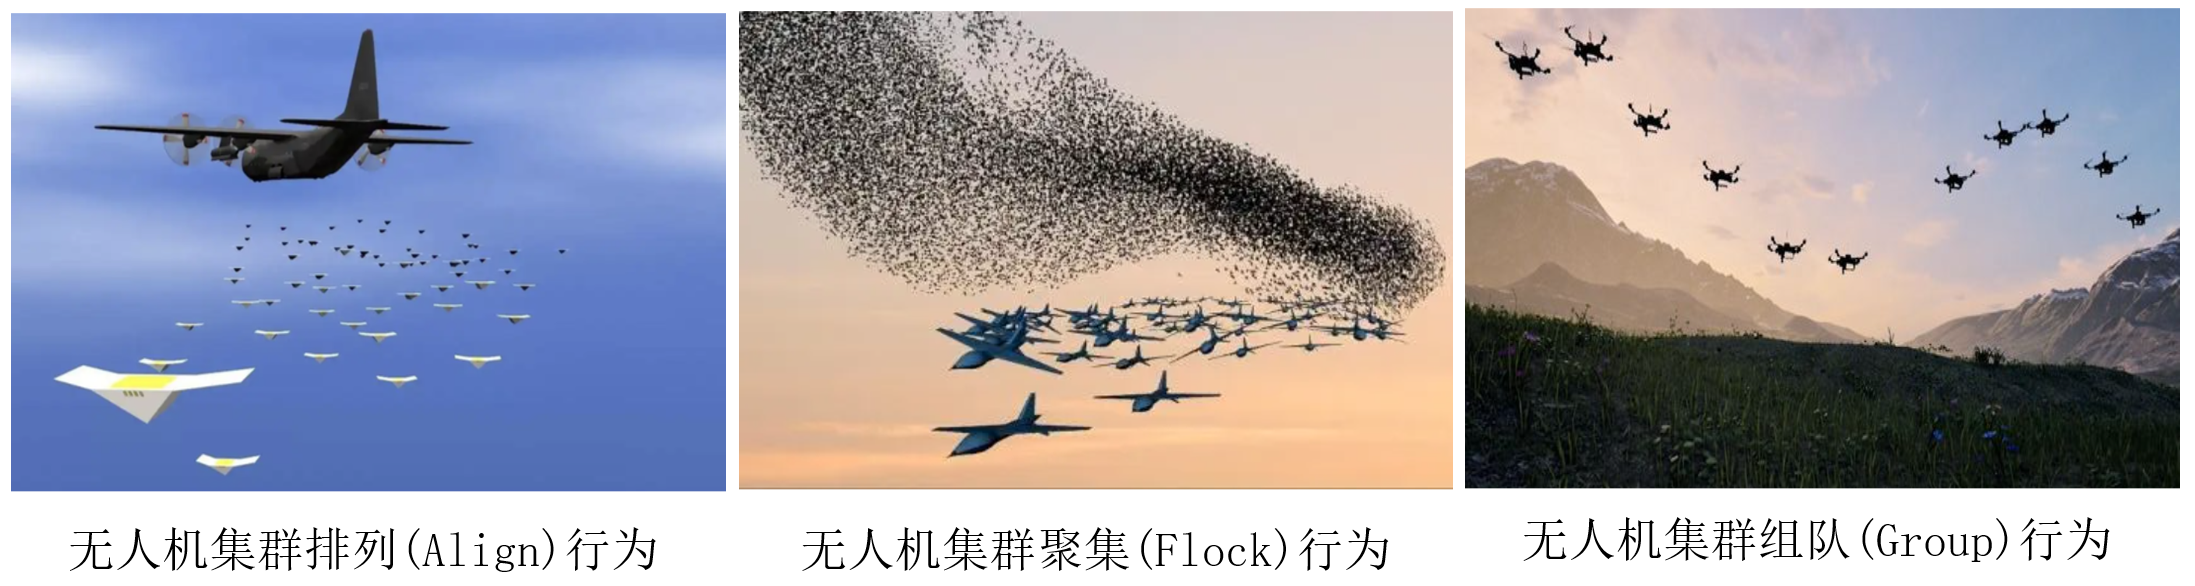
\includegraphics[width=1\linewidth]{Img/chapter0/swarm.png}
\caption{无人机集群若干典型行为示意图}
\label{fig:swarm}
\end{figure}

无人机集群系统在不同行为模式下可携带不同类型任务意图。通常而言, 无人机集群系统的行为与特定的任务分配具有一定的关联性, 对无人机集群行为的预判能够为无人机集群意图判别分析提供可用信息。例如, 在侦察任务下为躲避对方障碍物干扰, 无人机集群系统通常可采用排列(Align)行为; 在执行编队任务下无人机集群系统通常可通过聚集(Flock)行为或组队(Group)等行为模式达成任务目标。因此, 对无人机集群行为的分类研究可以为无人机集群意图推演和任务划分匹配提供前期的信息辅助, 是值得进行科研探索的方向之一。

无人机集群行为分类问题是指针对空中蜂群无人机整体行为的研究。当分布式无人机整体采取某种战略性和动态机动形式时, 无人机集群行为分类需要借助机器学习算法识别无人机集群行为模式并为未知无人机集群整体给出预测的行为类别\citep{Chung2018}。在先前的研究中, \citet{Hamann2018}提出针对无人机集群行为机器学习算法可以提供快速高效的分类结果。\citet{Brown2014}考察受限带宽约束条件下利用机器学习算法展开无人机集群行为分类。\citet{Brown2016DiscoveryAE}提出在单个无人机容量受限约束条件下利用机器学习算法开展集群行为分类问题。 \citet{Berger2016}提出降维算法将无人机集群行为数据压缩至低维线性子空间, 在低维线性子空间构建机器学习算法实现对无人机集群行为分类。 研究文献表明, 无人机集群相较于单个无人机可以完成更复杂的任务并且通过无人机集群的不同行为模式能够实现更丰富的目的意图推演\citep{Olaronke2020,Schranz2020}。 为此, \citet{Thomas2021}借助非线性时间序列预测模型探索无人机集群行为的特定对称性和动态特性之间的关系,并比较多种机器学习算法对于无人机集群行为预测效果。

\section{相关技术研究进展}
\subsection{无人机集群行为分类研究进展}
近些年的研究表明, 借助机器学习算法能够实现无人机集群行为分类。例如, 2014年美国空军动力研究院的\citet{Becker2014}采用压缩子空间学习技术结合机器学习算法实现无人机集群系统的行为判别。 他们将无人机集群整体的位置域信息和对应的无人机集群行为类别作为输入变量, 构建基于支持向量机模型的监督学习算法实现对无人机集群行为判别。\citet{Khan2020}于2018年提出采用混合人工判断的粒子行为判别实现无人机集群行为分类。 \citet{Hahn2019}在2019年提出采用增强学习理论进行无人机集群行为判别。2020年\citet{Lan2020}提出采用朴素贝叶斯, 高斯过程等统计学理论实现无人机集群行为分类。 

以上关于无人机集群行为分类的研究中, 大都基于无人机集群位置信息作为算法输入, 借用现代机器学习算法实现无人机集群行为分类。然而, 在许多机器学习算法应用中, 机器学习算法只会给出单值预测结果, 这种单值简单预测通常难以满足实际工程的需要。因此, 对机器学习算法输出结果给出可信程度的有效评估或者提供多类别输出的集合预测是非常重要的研究方向之一。

无论是对预测结果的可信评估还是集合预测, 这样的预测结果在理论上都属于对机器学习算法的不确定量化展开研究。对于许多风险敏感的科学研究领域, 例如医疗诊断\citep{Nouretdinov2013}、安全防卫\citep{Vineeth2014}及药物研发\citep{Janette2022}等领域, 给出机器学习输出结果的有效不确定量化预测是非常可取的。

主流学习算法中有两个主要领域可用于获得不确定量化研究, 分别是贝叶斯理论和“概率”近似正确理论(Probably Approximately Correct, PAC)\citep{Valiant1984}。 为应用贝叶斯框架, 需要具备一些关于数据生成的先验分布知识。 当有关数据分布的一些先验知识已知时, 贝叶斯方法可提供有效的最优决策。 然而, 对于经验推理科学\citep{Vapnik2006}并不具备有关分布的各种先验知识。 因此, 通常人们必须假设存在一个通用的规则, 进而在假设的通用规则下再展开问题的阐述。

历史上, 概率近似正确学习理论可以提供结果输出的不确定量化。 根据PAC学习模型, 首先预设犯错概率, 理论上要求保证在$1-\epsilon$概率下, 经验错误率小于等于$1-\epsilon$。 然而, 在具体现实研究中, 已有的结果已经表明, 概率近似正确理论下经验预测错误率边界往往远远超过$1-\epsilon$\citep{vovk2005algorithmic}。 同时, 概率近似正确学习理论对样本量需求巨大, 对噪声样本的容忍度较低, 模型的不确定量化结果鲁棒性较差\citep{vovk2005algorithmic}。 此外, 概率近似正确学习理论只能从整体上对预测的不确定进行评估和保证, 无法为每个样本提供不确定评估\citep{vovk2005algorithmic}。 因此, 基于概率近似正确学习理论的不确定量化, PAC学习理论通常无法得到有效保证\citep{Papadopoulos2008}。

对于其他传统概率预测算法, 如朴素贝叶斯(Na\"{i}ve Bayes)和逻辑回归(Logistic Regression)等传统统计模型, 其能够为每个个体预测结果提供不确定量化。 然而这些算法同样需要基于假设的概率分布展开。 然而严格说来, 传统统计和贝叶斯学习模型并不是“基于分布”展开数据分析, 而是“基于假设的分布”展开数据分析。 当数据符合假设的概率分布时, 贝叶斯学习的输出结果正确并且有效。 但如果数据不符合假设的概率分布, 尽管可以得到不错的预测结果, 但从理论上这些实用的结果大都无法得到有效保证的不确定量化结果\citep{vovk2005algorithmic}。

综上所述, 目前大多数机器学习算法仅仅给出预测结果, 但缺乏对预测结果提供有效不确定程度的考核。从理论角度审视这一问题, 即现有机器学习技术对每个预测结果无法提供有效的不确定量化\citep{2006Hedging}。

对于具有实际应用背景要求的无人机集群行为分类问题, 如何为机器学习算法的输出结果提供有效的不确定量化仍然面临着较大的挑战。在实际无人机集群行为分类研究中, 由于单一目的意图完全有可能采用多种无人机集群行为来实现, 因此有必要为无人机集群行为提供多类别集合预测。其次, 针对无人机集群行为分类问题, 由于真实数据本身的分布会随着时间发生变化, 基于前一种分布训练得到的学习模型难以继续为分布发生变化后数据提供高效预测, 因此有必要针对实际无人机集群数据提供一种有效的分布漂移检测\citep{Vovk2003,Vovk2012}。同时, 针对无人机集群数据稀缺的特点, 有必要开展小样本下无人机集群行为高效辨识研究\citep{Vapnik2009}。因此有必要针对上述科学问题开展研究。

\subsection{一致性预测方法研究进展}
Vapnik和Chervonenkis提出的统计学习理论提供一种基于纯粹数据驱动的无分布假设要求的新推理范式\citep{vapnik1974,vapnik1979,vapnik1982,vapnik1984,vapnik1995,vapnik1998,Vapnik2006,Chervonenkis2013}。 在这种新推理范式下, 通过控制两个因素(最小化经验风险泛函和诸函数的集合的容量)实现学习机器的构建。 统计学习理论是现象学学习模型\citep{Vapnik2019,Vapnik-context-2021,Vapnik-deep-2018,Vapnik-rethinking-2018}, 通过现象学还原\citep{vapnik2021-priviate-communication}可知学习机器的输出是一种暴力得分函数\citep{vapniktalk2015}, 不具备任何可信程度的度量\citep{2006Hedging}。 

一致性预测(Conformal Prediction, CP)是基于统计学习理论思想提出的一种无分布假设的可信机器学习解决方案\citep{vovk2005algorithmic}。 该算法框架由Vladimir Vovk, Alexander Gammerman和Glenn Shafer共同提出\citep{vovk2005algorithmic}, 它可以应用于任何学习算法之上来构建无分布假设的不确定度量。 与提供平均度量效果的传统统计方法不同, 一致性预测方法可以为单个个体提供有效的不确定度量指标。一致性预测提供置信度和可信度两种量化指标, 其中, 置信度衡量学习算法给出预测结果的可能性, 可信度衡量测试示例分类结果的适合程度。 与贝叶斯方法和PAC理论相比, 一致性预测方法给出的是有限样本下概率保证的有效不确定度量\citep{Poggi2017}。

一致性预测方法最初是在超越推理(Transductive Inference)范式\citep{vovk2021-priviate-communication}为机器学习算法的预测结果提供可靠评估的一套框架\citep{gammerman1998,soton1999,Saunders1999}。 基于柯尔莫哥洛夫概率论\citep{Kolmogorov1933,Kolmogorov-en-1956}, 在柯尔莫哥洛夫算法复杂度基础上\citep{Kolmogorov-en-1931-analytical,Kolmogorov-en-1946-leastsquare,Kolmogorov-en-1983,Kolmogorov-en-1991,Heidegger1966}结合Vapnik提出的支持向量机理论\citep{Cortes1995,vapnik1998}, Vovk将支持向量机理论中的支持向量的概念转译为置信预测, 这样在理论上就可以基于对冲预测提供一种可信赖的统计推断\citep{vovk2005algorithmic,2006Hedging}, 即对于给定训练数据集和新的观测数据, 可以基于一致性预测构建预测目标的置信区间。

采用一致性预测算法, 可以解决机器学习这类黑箱算法预测的不确定量化等科学问题。 传统机器学习算法是能够实现集群行为分类任务的, 其分类准确性度量一般建立在对测试数据预测能力的总体考核上, 其通用的评估方式(如均方误差类指标)大都采用对测试数据的平均汇总误差来表征算法的预测性能。 通用方法无法为单个样本的预测表现提供量化评估。 然而, 对于无人机集群行为判别这类高风险、低容错的研究任务需求, 采用常规意义上的整体误差评价指标无法为这类实际工程提供充分的不确定量化信息支持。 因此, 在本研究中需要考虑为无人机集群的单个预测输出提供有效的不确定量化, 并基于此实现机器学习黑箱算法的不确定量化。 

一致性预测是很有弹性的算法框架, 可以将一致性预测视为一种“刷子算法”, 任何机器学习算法经过改造都可以作为一致性预测的底层算法。 一致性预测算法能够对底层算法的输出“刷”上不确定量度, 并且其提供的不确定度量的有效性可以从理论上自动得到保障。 一致性预测成为学习理论的一个新方向并且是统计学习理论研究中的一种新的范式\citep{2006Hedging}, 因为一致性预测提供的不确定量度是基于有限样本的断言, 其不会考虑任何渐近的应诺式解决方案\citep{vovk2005algorithmic,2006Hedging}。

%
%一致性预测针对具体应用背景的特点, 结合统计学习理论为机器学习算法输出展开校正。 一致性预测对机器学习系统的预测结果提供可靠性评估和保障。 这种学习算法框架的优越性体现在如下几个方面: 首先, 一致性预测在对机器学习算法输出的每个个体的预测结果可以提供可靠性评估的同时能够确保整体预测结果的可靠性。 其次, 一致性预测框架提供的可靠性评估是有效的。 有效性是这一算法的重要性质。 再者, 一致性预测能够为任何机器学习算法提供有效的不确定度量。 特别重要的是, 区别于传统统计学总是基于渐近意义下得出的应诺(assure), 与之相反, 一致性预测的有效性不依托于渐近理论, 其阐述的有效性是在有限样本下给出的断言(assert)。 正是由于传统统计学算法无法提供有效估计, 这使得一致性估计在近几年越来越受到数据科学领域研究人员的关注。 

一致性预测在时间序列分析, 模式识别和回归分析领域都有大量的应用研究\citep{Vineeth2019}。\citet{Lei2015}提出采用一致性预测处理泛函数据分析任务, 并且给出无分布假设的统计推断方法。 \citet{Vovk2021retrain}提出使用一致性预测检测学习机器泛化推广能力的边界。\citet{Aleksandrova2021}通过大量实证研究说明一致性预测提供完整有效的不确定量化研究框架, 是解决现代机器学习不确定量化的重要研究方向。\citet{Victor2018}针对相依数据展开一致性预测研究, 提出一致性预测对于相依数据也能够提供精确的不确定量化结果。\citet{Xu2021}提出采用一致性预测算法为动态时间序列数据提供区间估计并且给出可行的解决方案。\citet{Dashevskiy2011}利用一致性预测方法为时间序列分类给出可信赖的预测。\citet{Papadopoulos2007}为神经网络提供一整套完整的基于一致性预测的不确定量化框架\citep{Papadopoulos2008}。\citet{Janette2022}提出针对临床医疗科学采用一致性预测方法提供不确定量化。

\subsection{分布漂移检测方法研究进展}

一致性预测的主要不足之处在于其前提建立在数据满足独立同分布假设上\citep{Finetti1975}。 在机器学习实际应用中, 研究者大都会随机将数据采样为训练集和测试集, 这样技术层面的操作一方面使得在建模时所用数据符合独立同分布假设的要求, 另一方面通过随机化采样数据使得训练模型在处理后数据上表现出相当优越的泛化学习推广能力。 然而在某些特定领域由于数据资源本身的稀缺特点以及研制问题本身的要求, 这就使得在需要面对数据本来的顺序时, 一致性预测的效率有所降低。

在处理实际应用问题时, 由于无法提前随机化数据, 数据的分布会随着时间发生变化。因此, 有必要给出关于数据本身分布的漂移检测度量标准。 分布漂移检测是统计学研究的重点, 但是仔细考察就会发现统计学将这一问题巧妙地归约为处理假设分布的漂移检测问题。 然而对于实际工程中的数据分析任务, 研究者通常并不能先验地给出任何关于分布的假设。 因此, 传统统计学给出的方法就始终扭结在到底如何提供很好的分布假设这一困境中\citep{Breiman2001,Efron2020}。

为解决上述问题, \citet{Vovk2003,Vovk2021retrain}提出一种无分布假设的分布漂移检测理论。根据此理论, 可以在各种应用背景下展开对研制问题数据本身分布的漂移检测。例如, \citet{Ho2005}使用此方法解决时变数据流的异常检测问题; \citet{Ho2012}应用鞅序列检测方法为高维时变数据流的可交换性提供一种端到端的解决方案; \citet{Ho2019}则将鞅序列方法应用于飞行轨迹的异常检验问题。 \citet{Vovk2012}提出一种基于“Plug-In”方法的分布漂移检测理论并将之应用于解决实际问题中的分布漂移检测。 这些实际的应用都已经表明采用无分布假设的分布漂移检测理论能够为实际问题提供优质的解决方案。 然而, 在无人机集群行为分类问题中还没有文献关注集群行为分类任务中分布漂移检测问题。 


\citet{Vovk1993}提出这种无分布假设的分布漂移检测方法利用机器学习的输出来实现对数据本身分布的检测。这种方法首先需要根据机器学习算法的输出构建鞅序列。而根据Vapnik-Chervonenkis理论, 机器学习算法属于现象学学习模型, 这种学习模型无需任何分布假设。 因此, \citet{Vovk1993}提出检测方法可以直接地检测“数据本身的分布漂移”, 而并不是检测“假设的分布漂移”。

综合目前研究结果和无人机集群研究的现实需要, 本文提出一种无分布假设的分布漂移检测方法, 这种方法能够为超高维数据提供端到端的分布漂移检测方案。这种方法无需任何先验知识, 仅仅依靠底层学习算法的输出, 构建得到的鞅序列即可完成分布漂移检测任务。 因此这种方法对于处理复杂无人机集群行为问题提供一种全新的分布漂移检测和预报方案。


\subsection{使用特权信息学习方法研究进展}

以上研究内容中所提出的方法都建立在机器学习算法的输出而展开。因此, 上述研究都依赖于底层机器学习算法的数据压缩能力。不难发现, 现有机器学习算法大都建立在大样本基础之上。然而, 考虑到无人机集群问题的实际应用背景, 有必要开展在小样本下的机器学习算法研究。

使用特权信息学习(Learning Using Privileged Information, LUPI)是机器学习领域中具有里程碑式的一种新学习范式\citep{Vapnik2009}。这种学习范式使得在机器学习领域能够提供直观学习\citep{Lerner1972,Ewald1996-1,Ewald1996-2}, 并且提供一种在小样本下的确保达到高精度的预测算法。特权信息的特点是其只能在训练阶段可用而在测试阶段不可用, 并且有效的特权信息需要研究者对所研问题提供整体描述信息\citep{Vapnik2006}。根据LUPI理论证明, 采用LUPI算法能够明显加速学习算法的收敛速度, 使得小样本下获得高精度的预测效果成为可能\citep{Pechyony2010}。

近些年, 使用特权信息学习模型在很多实际应用领域中得到广泛关注。 例如在特征选择研究中, \citet{Izmailov2018}基于$L_{1}$范数稀疏约束的LUPI范式下构建特征选择分类器。基于LUPI范式的特征选择能够扩充训练阶段的特征尺度, 从而显著提升机器学习算法的预测性能。为解决人机交互中潜变量的获取, \citet{Vrigkas2017}提出利用LUPI算法构建现代人机交互学习模式, 将研究者提供的直观信息输入学习算法来增强模型的稳定性。 在\citet{Vapnik-similary-2015}的工作中, Vapnik提出更新后的LUPI算法, 这种算法通过特权信息控制学习机器的容量从而加速学习算法的收敛。 \citet{Lapin2014}将LUPI算法的思想纳入SVM+框架, 同时引进二次优化算法实现所研问题的求解。 在许多实际应用问题研究中, 作者提出一种基于LUPI的问题求解器处理各种实际问题。 例如, \citet{Li2016}提出基于SVM+的特权信息模型解决各种预测和模式识别问题。\citet{Zheng2017}将LUPI框架应用医学影像诊断来实现小样本下高效分类的目标。

\section{研究内容与安排}
基于以上研究背景和技术进展状况, 从提高无人机集群行为分类的可信赖机器学习出发, 本文对无人机集群可信行为分类, 无人机集群分布漂移检测和小样本下无人机集群高精度分类设计进行研究。论文共分为\ref{chapter:conclusion}章。第\ref{chap:introduction}章是全文的背景介绍和问题引出。第\ref{chap:edbed}章是全文的理论基础。第\ref{chap:Swarm-MCP}章展开的是无人机集群行为分类的可信机器学习研究, 针对机器学习算法提出一种有效的不确定量化。第\ref{chapter:swarm-distributions}章和第\ref{chapter:swarm-martingales}章是针对无人机集群行为数据分布漂移相关内容展开的研究。针对无人机集群行为数据本身的分布随时间发生变化的现实, 本文研究如何在无分布假设的要求下开展分布漂移检测。针对检测到的分布漂移信息, 本文提出采用鞅保护分布算法来增强底层学习算法的预测性能。第\ref{chap:intelligent-learning}章是为小样本下无人机集群行为分类提出一种全新的学习范式。在小样本训练要求下, 本文提出使用特权信息学习方法加速学习算法收敛, 使得在无人机集群行为分类中通过提供整体描述实现小样本下高精度预测。第\ref{chapter:conclusion}章为总结与展望。本文研究框架如图\ref{fig:thesis-frame}所示, 在研究框架图中单列每一章节研究的主题词, 各章主要内容如下:

\begin{figure}
\centering
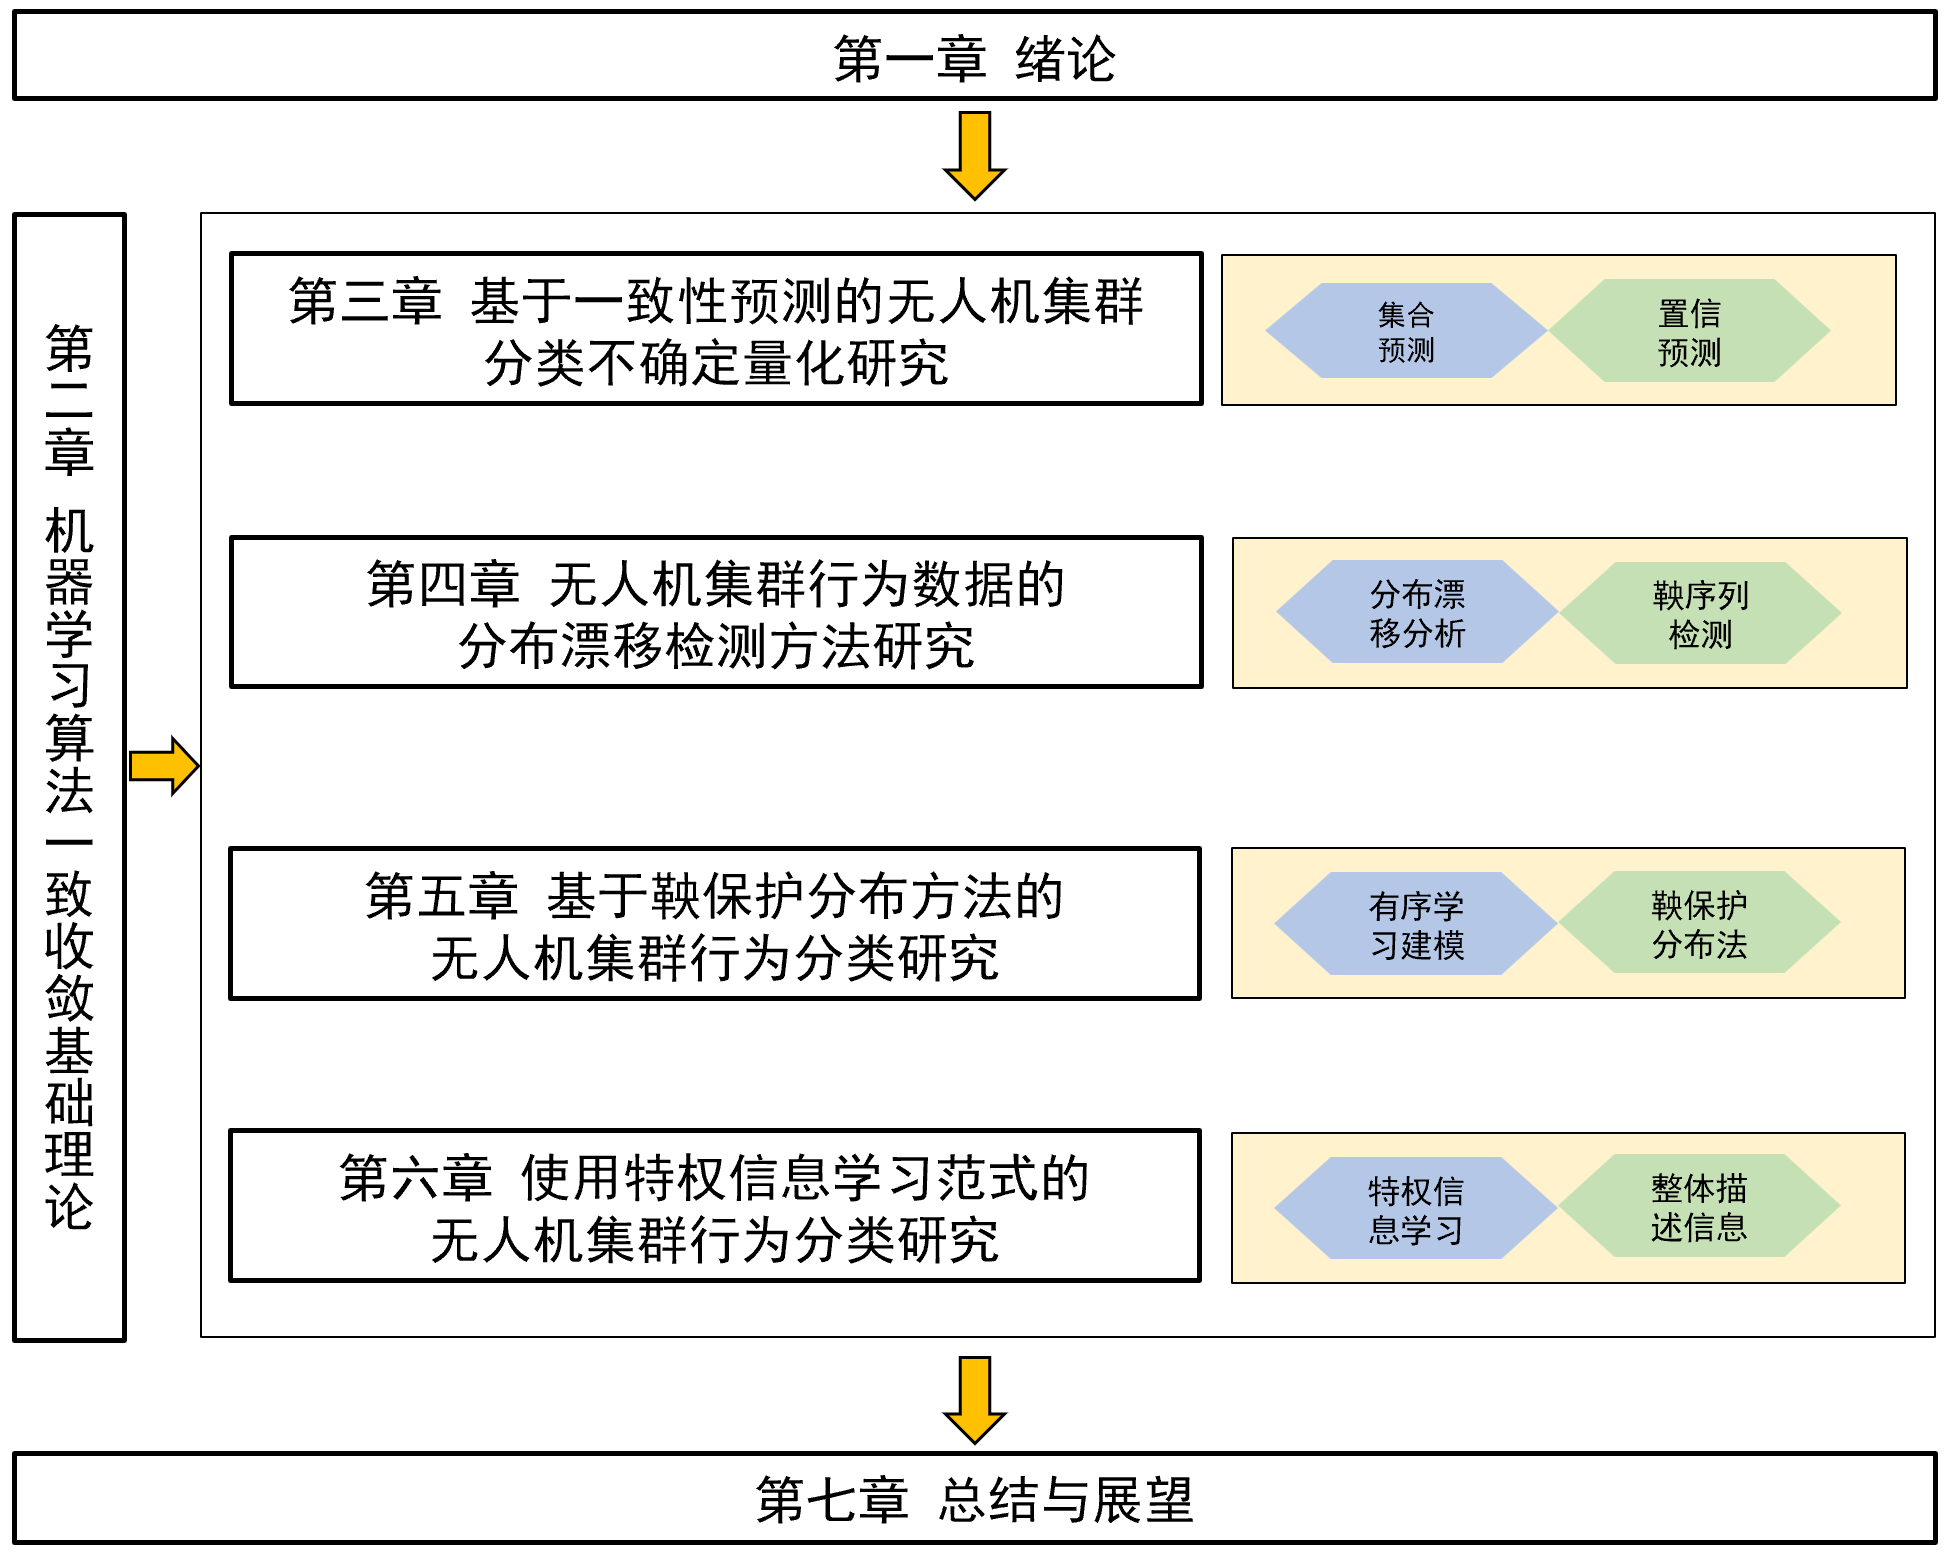
\includegraphics[width=.9\linewidth]{Img/thesis-frame}
\caption{论文组织结构图}
\label{fig:thesis-frame}
\end{figure}

第\ref{chap:introduction}章, 绪论。首先介绍论文的研究背景与意义, 然后从一致性预测方法、分布漂移检测方法和使用特权信息学习三个方面概述现有方法的研究进展。

第\ref{chap:edbed}章, 介绍统计学习理论基础, 着重强调机器学习算法的现象学学习模型基础。本文指出需要控制两个因素: 其一是经验风险最小化, 其二是学习机器的容量来使得学习问题的一致收敛条件成立。根据统计学习理论可知, 以上控制学习问题收敛的两个因素唯一受VC维的控制。 因此, 在后续实际应用中要始终围绕如何控制容量展开研究, 并且突出强调Vapnik-Chervonenkis理论给出的关于学习理论的阐述是一种断言式的解答而不是应诺式的言说。由于本文的工作都在机器学习算法的顶层展开, 因此得出的结论都是有保证的可信赖推理结果。

第\ref{chap:Swarm-MCP}章, 在一致性预测的基础上提出改进后的蒙德里安一致性预测为复杂无人机集群行为的可信分类提供精确有效的统计推断。 本文为无人机集群行为分类提供两种精确有效的可信预测模型, 其一是精确有效的置信预测, 即为当前机器学习简单预测结果给出精确有效的置信度度量和可信度度量; 其二, 为复杂无人机集群行为分类提供一种精确有效的有保证的集合预测。 与此同时, 针对每一种预测结果本文都检验预测结果的有效性, 这些精确检验算例验证所提方法的可行性和有效性。

第\ref{chapter:swarm-distributions}章, 在一致性预测基础上开展无人机集群分布漂移检测研究。 本文注意到构建常规机器学习算法时一般默认将整个数据集随机采样得到训练集和测试集合, 然后用训练集训练机器学习算法并在测试集合上检验此算法的预测效果。根据现代概率论相关知识, 借助技术随机化经验数据能够使得处理数据满足模型前提假设, 但同时会消除数据本身的某些重要的分布信息。 为此本文提出一种无分布假设的鞅序列方法检测数据本身的分布信息。所提方法是在机器学习算法输出结果之上展开的, 是一种能够处理超高维数据、无任何分布假设先验要求的分布漂移检测方法, 能够对分布漂移检测问题提供端到端的高效检测。最后,通过真实无人机集群行为数据集验证所提方法的可行性和有效性。

第\ref{chapter:swarm-martingales}章, 通过采用鞅保护分布方法将鞅检测理论与机器学习算法相结合, 并提出利用鞅保护分布理论改进底层学习算法的完整框架。将鞅保护分布算法纳入考量之后, 真实数据的分布漂移信息就可以加入训练模型, 因此本文提出的算法能够增强原先学习算法的泛化推广能力。 本文将提出的鞅保护分布算法应用于多种机器学习算法之上, 通过三种公开的真实无人机集群行为数据集分别测试所提出的算法。试验结果证明, 所提方法对各类底层机器学习算法大都具有显著的提升, 同时也验证所提鞅保护分布算法的可行性和有效性。

第\ref{chap:intelligent-learning}章, 提出一种新的学习范式(即使用特权信息学习)处理小样本下无人机集群行为分类问题。特权信息是在训练阶段可用, 但是测试阶段不可用的整体描述信息。首先, 选取无人机集群中个体间合作描述信息作为特权信息, 阐述在合作描述信息作为特权信息模型下, 无人机集群行为分类实现小样本训练而达到高精度预测能力的模型。其次, 选取无人机集群个体间竞争描述信息作为特权信息, 阐述在竞争描述信息作为特权信息模型下, 无人机集群行为分类实现小样本训练而达到高精度预测能力的模型。本文将这两种模型分别应用于三种公开无人机集群行为数据, 分别检验特权信息在三种无人机集群行为数据集下的预测效果, 试验结果证实所提基于特权信息学习模型方案的可行性和有效性。

第\ref{chapter:conclusion}章对全文内容进行总结并给出进一步研究的展望。
\chapter{机器学习算法一致收敛基础理论}
\label{chap:edbed}
\section{引言}
本章给出机器学习算法一致收敛基础理论, 这些理论对于后续章节中阐述具体算法起到至关重要的指导作用。因为后续章节的工作都建立在机器学习算法的输出结果之上而展开的研究, 所以对于具体机器学习算法并不会展开详细的介绍, 仅仅从理论层面对底层机器学习算法给出分析。

关于机器学习算法的理论阐述, 最后归约为基于经验数据的相依关系估计问题\citep{vapnik1982}。这一问题由Vapnik和Chervonenkis完整给出\citep{vapnik1974,vapnik1979,Vapnik2006,Chervonenkis2013}。Vapnik公理化定义“模式”, 给出“识别”的定义并且提出采用“广义肖像法”实现模式识别问题的解答\citep{vapnik1962,vapnik1963,vapnik1964On,vapnik1964}。对于泛函依赖关系估计问题, 按照泛函分析理论都抽象为相同的模型来考虑, 即在所有可能的依赖关系中需要找到某函数关系, 此函数关系是满足给定量化评价标准下的最佳函数关系。形式化而言, 即对于向量空间 $Z$, 诸函数的集合 $\{g(z), z \in Z\}$所有可能的依赖关系的类是给定的。定义某泛函表达式
\begin{align}\label{1.1}
I = I(g)
\end{align}
作为选择依赖关系的量化指标。那么需要在集合 $\{g(z)\}$ 中搜索使得泛函 (\ref{1.1}) 最小化的函数 $g^{*}(z)$。在这种情形下,当给出函数集合$\{g(z)\}$和泛函$I(g)$的确切数学表达式时, 寻找使泛函$I(g)$最小化的函数$g^{*}(z)$的问题就转化为变分法的求解问题\citep{Hilbert1950,mmp-1953,mmp-1962,Marx1881}。

然而就学习问题而言, 统计学习理论将之归约为根据经验数据的相依关系估计问题\citep{vapnik1974,Faffelberger1980}。即在所有可能的泛函依赖关系中选择一个在满足给定的量化评价标准下最优函数(诸函数是由机器实施的)。形式化而言, 即当概率密度函数$P(z)$定义在向量空间$Z$, 泛函关系定义为下列数学期望
\begin{align}\label{1.2}
I(g) = \int \Phi(z,g(z))P(z)dz.
\end{align}
那么所考虑的问题就是当概率密度函数 $P(z)$未知, 但已知观测样本
\begin{align}\label{1.3}
z_1,\ldots,z_l
\end{align}
来源于服从密度函数$P(z)$的随机独立试验时,最小化泛函 (\ref{1.2})的问题。

对于最小化期望风险泛函问题, 诸函数的类 $\{g(z)\}$是以参数形式$\{g(z,\alpha)\}$给出的, 其中这里参数$\alpha$是属于集合$\Lambda$的。对于具体的参数取值$\alpha = \alpha^{*}$, 其定义属于函数类$g(z,\alpha)$的某具体函数$g(z, \alpha^{*})$。就学习问题而言, 搜索所需函数等同于确立所求参数$\alpha$的值。特别需要指出的是, 问题的研究并不局限在仅由某几个参数确定的函数类, 而是集合 $\Lambda$ 的参数 $\alpha$ 可以是任意的, 比如可以是诸标量的集合,或者诸向量的集合,也可以是任意抽象元素的集合。例如在神经网络中,这里的集合 $\Lambda$就是网络节点的集合。

现在可以将泛函(\ref{1.2})重新用新的术语写出, 即
\begin{align}\label{1.4}
I(\alpha) = \int Q(z,\alpha)P(z)dz, \alpha \in \Lambda,
\end{align}
其中,
\begin{align}
Q(z,\alpha) = \Phi(z,g(z,\alpha)).
\end{align}
这里的函数 $Q(z,\alpha)$称为损失函数。

现在考虑具体的情况, 即向量空间 $z$ 有$n+1$ 个坐标, 其中分别是标量 $y$ 以及 $n$ 个坐标的数据向量 $x$。损失函数 $Q(z,\alpha)$ 按下列表达式给出
\begin{align}
Q(z,\alpha) = \Phi(y - F(x,\alpha)),
\end{align}
其中,这里函数 $F(x,\alpha)$ 是参数化的诸函数的类。现在的问题是最小化下列泛函
\begin{align}\label{1.5}
I(\alpha) = \int \Phi(y-f(x,\alpha))P(x,y)dxdy
\end{align}
而所面对情形是这里的概率密度 $P(x,y)$ 未知, 但随机独立的训练序列样本给定
\begin{align}\label{1.6}
x_1,y_1; \ldots; x_l,y_l.
\end{align}

将基于经验数据(\ref{1.6})来最小化泛函(\ref{1.5})的问题称为基于经验数据的相依关系估计, 亦称作统计学习问题。


统计学习问题的理论阐述是20世纪50年代末期提出\citep{Rosenblatt1962,Novikoff1962,vapnik1963,vapnik1964,vapnik1964On,vapnik1968,vapnik1971,vapnik1974,vapnik1979}, 这一类问题的数学形式化可以表述为:按照图 \ref{fig:power-right}所示, 这里有三个要素:
\begin{enumerate}
\item 数据的生成器 $G$,
\item 目标算子或监督器 $S$,
\item 学习机器 $LM$。
\end{enumerate}

统计学习理论中关于机器学习算法的学习问题设定属于现象学学习模型\citep{Vapnik-rethinking-2018,wangdefeng2005}, 即在由概率密度函数 $P(x)$ 所刻画的环境条件下, 数据 $x$ 随机且独立地出现, 学习机制是把数据划分为 $k$ 个不同的类别。假设学习机器按照条件概率分布函数 $P(y | x), y = \{0,1\}$, ($y=0$ 表示将 $x$ 划分为第一类,  $y=1$ 表示划分为第二类)进行分类。给定参数化泛函集合 $F(x,\alpha)$和观测到的$l$对数据
\begin{align}
x_1, y_1; \ldots; x_l, y_l,
\end{align}
其中, 这里的$x$表示学习环境, $y$为学习反馈。学习过程就是在集合$F(x,\alpha)$中选择一个函数使得其分类错误的概率是集合中其他分类器中最小的。也就是说, 必须取得下列泛函的最小值
\begin{align}
I(\alpha) = \int_{X,y}^{} (y - F(x,\alpha))^2P(x,y)dxdy.
\end{align}
其中,这里的函数$P(x,y) = P(y | x)P(x)$ 是定义在空间$X, y$上的关于数据对$x, y$的联合概率密度函数。这样一来学习问题被归约为基于经验数据的最小化期望风险问题。

\begin{figure}
\centering
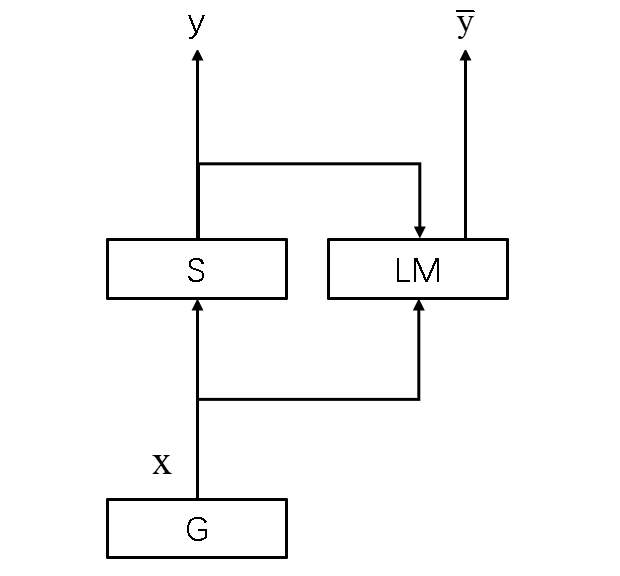
\includegraphics[width=.4\linewidth]{Img/chapter1/power-right.png}
\caption{现象学学习理论模型示意图}
\label{fig:power-right}
\end{figure}

\section{将学习问题归约为最小化经验风险泛函问题}
统计学在处理这一问题时,将此问题与估计诸概率密度函数问题相关联。按照统计学处理思路, 下列期望风险泛函
\begin{align}\label{ch6.1}
I(\alpha)=\int(y-F(x, \alpha))^{2} P(x, y) d x ~d y
\end{align}
在基于下列经验数据
\begin{align}\label{ch6.2}
x_{1}, y_{1} ; \ldots ; x_{l}, y_{l}
\end{align}
最小化的问题被归约为基于样本数据(\ref{ch6.2})估计密度函数$\hat{P}(x,y)$, 然后再求解关下列泛函的最小化问题
\begin{align}
I_{\mathrm{emp}}(\alpha)=\int(y-F(x, \alpha))^{2} \hat{P}(x, y) d x ~d y.
\end{align}

\citet{vapnik1982}已经完整阐明, 用这种方法最小化风险泛函(\ref{ch6.1})通常是不合理的。因为相较于最小化期望风险(\ref{ch6.1}), 密度函数的估计问题通常是更艰难的问题。只有当拥有关于这一密度函数$P(x,y)$足够多的、可用的先验信息时, 函数$P(x,y)$的参数方才有可能确定, 此时传统统计学的方法才能够勉强的、似是而非的执行\citep{Vapnik2006}。然而对于特定的现实问题其密度函数$P(x,y)$是未知的, 因此统计学处理这一问题就始终扭结在如何提供一个很好的密度函数的假设上。

统计学习理论处理这类问题则无需任何分布假设。统计学习理论的基本原则是对于最小化期望风险泛函问题, 当期望风险泛函(\ref{ch6.1})取得最小值的时候, 由随机独立样本(\ref{ch6.2})构建的下列经验风险泛函
\begin{align}\label{ch6.3}
I_{\mathrm{emp}}(\alpha)=\frac{1}{l} \sum_{i=1}^{l}\left(y_{i}-F\left(x_{i}, \alpha\right)\right)^{2},
\end{align}
也取得最小值。令经验风险泛函(\ref{ch6.3})取得的最小值为 $F(x,\alpha_{emp})$。那么关键的问题就是要阐明, 到底在什么时候, 经验风险泛函的最小值$F(x,\alpha_{emp})$能逼近期望风险泛函的最小值$F(x,\alpha_0)$, 而后者正好就是在函数族$F(x,\alpha)$中能够最小化表达式(\ref{ch6.1})的所求函数。针对这一问题成立的条件, 就是学习问题的一致收敛条件, 本文会分别从有限决策规则和无限决策规则两种情形下给出学习问题的一致收敛条件。

\section{有限决策规则下学习问题一致收敛条件}
\label{sec:uniform-convergence}
现在考虑学习问题一致性收敛的条件, 先从有限规则情形展开阐述, 进而将之推广至无限规则情形。

考虑下列期望泛函:
\begin{align}\label{ch6.10}
I(\alpha)=P(\alpha)=\int(y-F(x, \alpha))^{2} P(x, y) dx~dy.
\end{align}
正如已经阐明的, 此泛函定义的是每个决策规则分类错误的\textsf{概率}。而下列经验泛函
\begin{align}\label{ch6.11}
I_{\mathrm{emp}}(\alpha)=v(\alpha)=\frac{1}{l} \sum_{i=1}^{l}\left(y_{i}-F\left(x_{i}, \alpha\right)\right)^{2},
\end{align}
自然是通过下列样本
\begin{align}\label{ch6.12}
x_{1}, y_{1} ; \ldots ; x_{l}, y_{l},
\end{align}
计算得到的,此泛函定义的是每个决策规则分类错误的\textsf{频率}。

根据概率论经典理论, 当样本量增加至无穷时, 随机事件出现的频率收敛至此事件概率。形式化而言, 这意味着对于任意的$\alpha$和$\varkappa$, 下列关系表达式
\begin{align}\label{ch6.13}
\lim _{l \rightarrow \infty} P\{|P(\alpha)-v(\alpha)|>\varkappa\}=0
\end{align}
是成立的。然而, \citet{vapnik1982}已经阐明, 概率论推行的收敛表达式(\ref{ch6.13})的成立并不能保证最小化经验泛函(\ref{ch6.11})的那个决策规则, 其产生的关于期望泛函(\ref{ch6.10})的值就是期望泛函(\ref{ch6.10})的最小值。如图 \ref{fig:frequency} 所示的情形, 对于大样本情形下, 经验泛函$I_{\text{emp}}(\alpha)$与期望泛函$I(\alpha)$的差距的确能够收敛, 但是并不能以此就断言经验泛函$I_{\text{emp}}(\alpha)$取得最小值就能够保证也对应期望泛函$I(\alpha)$取得最小值。

对于大样本$l$的情况, 经验条件下所得问题解与期望最佳解之间的差距只有在满足一个更强的条件时才可以\textsf{断定}诸频率收敛至诸概率,即要求对于所有可能的情形, 都满足下列条件
\begin{align*}
|P_{1}(\alpha)&-v_{1}(\alpha)|>\varkappa,\\
|P_{2}(\alpha)&-v_{2}(\alpha)|>\varkappa,\\
&\ldots\\
|P_{N}(\alpha)&-v_{N}(\alpha)|>\varkappa.
\end{align*}
也就是说, 并不是要求统计学中用到的表达式(\ref{ch6.13})成立, 而是特别地要求下列表达式
\begin{align}\label{ch6.14}
\lim_{l \rightarrow \infty} P\left\{\sup _{\alpha}|P(\alpha)-v(\alpha)|>\varkappa\right\}=0
\end{align}
对于任意的$\varkappa$成立。此时称在所有随机事件的类$S(\alpha)$上这些事件的诸频率一致地收敛至诸概率, 将这样的表述记为“诸事件‘频率-概率’一致收敛”。这样一来, 对于在函数类$S(\alpha)$中的每个事件$S(\alpha^{*})$——此事件是由具体的决策规则$F(x,\alpha^{*})$给定的——就都满足等式$(y - F(x, \alpha^{*}))^{2} = 1$。

\begin{figure}
\centering
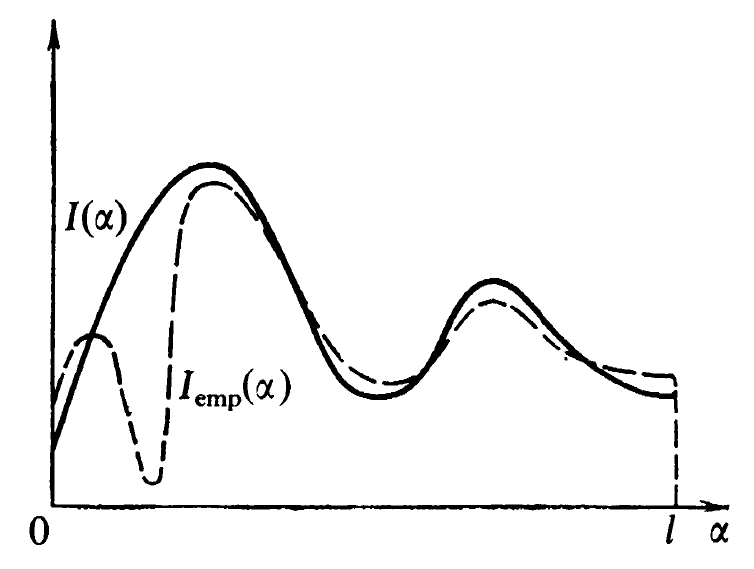
\includegraphics[width=.5\linewidth]{Img/chapter1/frequency.png}
\caption{机器学习理论一致收敛问题示意图}
\label{fig:frequency}
\end{figure}

\subsection{不可分情形下绝对偏差一致收敛的界}
\label{sec:special-case}

首先考虑不可分情形下“频率-概率”一致收敛的条件。考虑诸决策规则的类是由$N$个有限规则\footnote{这里的规则数目$N$是一个非常大的数 \citep{Lerner1980}。}组成的函数类$F(x;\alpha)$:
\begin{align}
F\left(x, \alpha_{1}\right), \ldots, F\left(x, \alpha_{N}\right).
\end{align}
对应每个决策规则$F(x,\alpha_i)$的随机事件$A_i$由数据对$x, y$组成, 且满足$(y - F(x,\alpha_i))^{2} = 1$。这就定义$N$个有限数量事件$A_1,\ldots,A_N$.

对于每个固定事件, 依照概率论易知大数定律自然是有效的, 即随着试验次数的无限增加, 此固定事件下的频率收敛至其概率。此大数定律的一个特例就是下列Hoffding不等式:
\begin{align}\label{ch6.15}
P\left\{\left|P\left(\alpha_{i}\right)-v\left(\alpha_{i}\right)\right|>\varkappa\right\}<2 \exp \left\{-2 \varkappa^{2} l\right\}.
\end{align}
然而, 要探究的核心在于要求一致收敛, 也就是说要求确保下列诸不等式同时满足的概率
\begin{align}
\left|P\left(\alpha_{i}\right)-v\left(\alpha_{i}\right)\right| \leq \varkappa, \quad i=1,2, \ldots, N.
\end{align}
如果对于表达式(\ref{ch6.15})中出现的每个不等式能够断言其可以独立分开评估的话, 那么一致收敛要求下的概率可以很容易地界定, 即可得
\begin{align}
P\left\{\sup _{i}\left|P\left(\alpha_{i}\right)-v\left(\alpha_{i}\right)\right|>\varkappa\right\} \leq \sum_{i=1}^{N} P\left\{\left|P\left(\alpha_{i}\right)-v\left(\alpha_{i}\right)\right|>\varkappa\right\}.
\end{align}
将不等式(\ref{ch6.15})带入,得到
\begin{align}\label{ch6.16}
P\left\{\sup _{i}\left|P\left(\alpha_{i}\right)-v\left(\alpha_{i}\right)\right|> \varkappa\right\}<2 N \exp \left\{-2 \varkappa^{2} l\right\}.
\end{align}
这个不等式就意味着, 对于有限数量的随机事件, 其“频率-概率”一致收敛始终有效, 也就是说其极限为
\begin{align}
\lim _{l \rightarrow \infty} P\left\{\sup _{i}\left|P\left(\alpha_{i}\right)-v\left(\alpha_{i}\right)\right|>\varkappa\right\}=0.
\end{align}

现在要求在特定事件的具体实现中,其对应的概率
\begin{align}
\left\{\sup _{i}\left|P\left(\alpha_{i}\right)-v\left(\alpha_{i}\right)\right|>\varkappa\right\}
\end{align}
不要超过$\eta$, 即要求下列表达式
\begin{align}\label{ch6.17}
P\left\{\sup _{i}\left|P\left(\alpha_{i}\right)-v\left(\alpha_{i}\right)\right|>\varkappa\right\}<\eta
\end{align}
需要成立。从不等表达式(\ref{ch6.16})中可以得到不等式(\ref{ch6.17})成立的条件是$N, l, \varkappa$ 和 $\eta$ 这些量化指标要满足下列关系式
\begin{align}\label{ch6.18}
2 N \exp \left\{-2 \varkappa^{2} l\right\}=\eta.
\end{align}
如果在表达式(\ref{ch6.18})中求解$\varkappa$, 那么对于给定的 $N, l$和$\eta$, 就得到在给定条件下的诸事件的类中, 诸频率与其概率的最大偏差的估计量就是
\begin{align}\label{ch6.19}
\varkappa=\sqrt{\frac{\ln N-\ln (\eta / 2)}{2 l}}.
\end{align}
然而, 如果在表达式(\ref{ch6.18})中解出$l$, 那么可以断言(assert), 至少以概率 (with probability) $1-\eta$ 在这个函数类上诸频率和诸概率的最大偏差不会超过$\varkappa$的样本的大小是:
\begin{align}\label{ch6.20}
l=\frac{\ln N-\ln (\eta / 2)}{2 \varkappa^{2}}.
\end{align}

因此证明下面的定理:
\begin{theorem}\label{theorem6.1}
\citep{vapnik1998}
设诸决策函数的集合包含$N$个元素, 对于决策函数$F(x,\alpha_i)$, 令在样本容量为$l$时分类错误的频率为$v(\alpha_i)$。那么, 以概率(with probability)$1-\eta$有可能断言(may assert)下列不等关系表达式,
\begin{align}
v\left(\alpha_{i}\right)-\sqrt{\frac{\ln N-\ln (\eta / 2)}{2 l}} \leq P\left(\alpha_{i}\right) \leq v\left(\alpha_{i}\right)+\sqrt{\frac{\ln N-\ln (\eta / 2)}{2 l}}
\end{align}
对于所有决策函数都同时成立。
\end{theorem}

\begin{remark}
因为以上不等式是对所有$N$个决策规则都成立, 因此定理 \ref{theorem6.1} 对于某个具体决策规则$F(x,\alpha_{\text{emp}})$——此规则在$N$个规则中能够最小化经验风险泛函——的品质确定其置信区间。这个置信区间就是
\begin{align}
v\left(\alpha_{\text {emp }}\right)-\sqrt{\frac{\ln N-\ln (\eta / 2)}{2 l}} \leq P\left(\alpha_{\text {emp }}\right) \leq v\left(\alpha_{\text {emp }}\right)+\sqrt{\frac{\ln N-\ln (\eta / 2)}{2 l}}.
\end{align}
\end{remark}

因为更关注决策规则的品质的上界, 即对于所有的决策规则, 以概率(with probability) $1-\eta$
\begin{align}
P\left(\alpha_{i}\right) \leq v\left(\alpha_{i}\right)+\sqrt{\frac{\ln N-\ln (\eta / 2)}{2 l}}
\end{align}
使得上面的不等式同时有效。

因此, 在决策规则有限情形下,一致收敛的要求不仅仅与最小化经验泛函$v(\alpha_{i})$有关, 还与决策规则的品质——即置信区间$\sqrt{\frac{\ln N-\ln (\eta / 2)}{2 l}}$——有关.

\subsection{可分情形下绝对偏差一致收敛的界}
\label{sec:kefen}
以上给出的是在一般决策规则有限的情形下考察的一致收敛问题。基于定理\ref{theorem6.1}计算得到的置信区间可能过于宽泛——因为在不可分情形下并不要求有限$N$个决策一定就包含那真实函数本身。

现在考虑可分情形下学习问题的一致收敛条件。因为在所有的决策函数$F(x,\alpha_i)(i=1,\ldots,N)$中确实存在着一个函数, 其能够完美地解决分类问题, 那么这就是一个明晰的先验知识, 即对于任意的样本其最小化经验风险泛函的值一定是0。然而, 这个最小值是可以通过好几个函数求得的。所以需要估计对于任意函数——这些函数都能够使得经验风险的最小值为0——其估计品质不超过给定的$\varkappa$的概率是多少。

引进函数
\begin{align}
\bar{\theta}(z)=\left\{\begin{array}{ll}
1 & \text { for } z=0 ,\\
0 & \text { for } z>0.
\end{array}\right.
\end{align}
那么, 在诸事件的集合上——在此集合上错误分类的频率为零——诸频率一致收敛至其概率的速度的估计, 就是针对下列事件的概率的估计
\begin{align}
\left\{\sup _{i}\left|P\left(\alpha_{i}\right)-v\left(\alpha_{i}\right)\right| \bar{\theta}\left(v\left(\alpha_{i}\right)\right)>\varkappa\right\}
\end{align}
(而并不是如定理\ref{theorem6.1}所述的针对事件$\left\{\sup _{i}\left|P\left(\alpha_{i}\right)-v\left(\alpha_{i}\right)\right| > \varkappa\right\}$的估计)。

因为对于那些使得经验风险取值为零的决策函数的数量不会超过$N$($N$是决策函数集合中函数的总数量), 所以下列不等式
\begin{align}\label{ch6.21}
P\left\{\sup _{i}\left|P\left(\alpha_{i}\right)-v\left(\alpha_{i}\right)\right| \bar{\theta}\left(v\left(\alpha_{i}\right)\right)>\varkappa\right\} \leq N P_{\varkappa}
\end{align}
总是成立的。其中, 这里$P_{\varkappa}$表征的是在所有样本中错误分类的误差超过$\varkappa$的概率。很自然地, 这一概率的界就由下列表达式给出
\begin{align}\label{ch6.22}
P_{\varkappa} \leq(1-\varkappa)^{l}.
\end{align}
将针对$P_{\varkappa}$的界带入表达式(\ref{ch6.21}), 得到
\begin{align}\label{ch6.23}
P\left\{\sup _{i}\left|P\left(\alpha_{i}\right)-v\left(\alpha_{i}\right)\right| \bar{\theta}\left(v\left(\alpha_{i}\right)\right)>\varkappa\right\} \leq N(1-\varkappa)^{l}.
\end{align}
为使得下列概率
\begin{align}
P\left\{\sup _{i}\left|P\left(\alpha_{i}\right)-v\left(\alpha_{i}\right)\right| \bar{\theta}\left(v\left(\alpha_{i}\right)\right)>\varkappa\right\}
\end{align}
不超过给定值$\eta$, 其充分条件便是下列表达式成立
\begin{align}\label{ch6.24}
N(1-\varkappa)^{l}=\eta.
\end{align}
从中求解$l$, 可得
\begin{align}\label{ch6.25}
l=\frac{\ln N-\ln \eta}{-\ln (1-\varkappa)}.
\end{align}
因为当$\varkappa$取较小值时, 下列近似表达式
\begin{align}
-\ln (1-\varkappa) \approx \varkappa
\end{align}
成立, 因此表达式(\ref{ch6.25})可以表示为下列形式
\begin{align}
l=\frac{\ln N-\ln \eta}{\varkappa}.
\end{align}
与表达式(\ref{ch6.20})不同的是, 这里得到的分母为$\varkappa$而不是先前得到的$2\varkappa^2$。这就是说, 在确定问题陈述中所需的样本量要比通常一般情况下的样本量少得多。在表达式(\ref{ch6.24})中求解$\varkappa$, 可以得到
\begin{align}
\varkappa=\frac{\ln N-\ln \eta}{l}.
\end{align}
这样便可以得到下列定理:

\begin{theorem}\label{theorem6.2}
\citep{vapnik1998}
如果在$N$个决策规则函数集合中可以选择出某一个规则,其能够使得样本分类不出错, 那么可以以概率(with probability)$1-\eta$断言(assert), 使用所选中的这一规则得到的错误分类概率的界为
\begin{align}
0 \leq P \leq \varkappa,
\end{align}
其中
\begin{align}
\varkappa=\frac{\ln N-\ln \eta}{l}.
\end{align}
\end{theorem}

从这里也可以看到, 即便是对于确定陈述问题, 最小化经验风险泛函的方法也不能够保证“频率-概率”一致收敛, “频率-概率”一致收敛仍然还要求控制决策规则的品质$\varkappa=\frac{\ln N-\ln \eta}{l}$。


\section{无限决策规则下学习问题一致收敛条件}
到目前为止, 已经在非常粗糙的层面通过使用“容量”来刻画诸决策规则的集合来得到“频率-概率”一致收敛速度的界(大概把“容量”等同于在此集合中诸元素的个数)。

在本节开始要引入一个更为精确的容量指标刻画量——样本大小$l$上诸事件的系统的熵。使用这一刻画指标可以全面而彻底详尽地阐发并建构随机事件“频率-概率”偏差一致收敛速度的充分必要条件, 即建构有关下列等式
\begin{align}
\lim _{l \rightarrow \infty} P\left\{\sup _{\alpha}|P(\alpha)-v(\alpha)|>\varkappa\right\}=0
\end{align}
对于任意$\varkappa$都成立的充分必要条件。

首先令诸决策规则$F(x,\alpha)$的集合$S$已被定义并且给定样本$x_1,\ldots,x_l$。这些样本一般说来当然可以按照$2^{l}$种方式划分为两类。然而, 只有可以使用诸规则$F(x,\alpha)$完成的那些划分才是感兴趣的。(也就是说, 感兴趣的是使用规则$F(x,\alpha^{*})$, 样本集合$x_1,\ldots,x_{l}$能够被划分为这样两个子集: 其一满足 $F(x,\alpha^{*})=1$, 另一集合满足$F(x,\alpha^{*})=0$。) 不同划分方法的数量依赖于诸决策规则$F(x,\alpha)$的类本身, 同时也依赖于样本。“不同划分方法的数量”这一指标记为
\begin{align}
\Delta^{S}\left(x_{1}, \ldots, x_{l}\right).
\end{align}

现在来考虑由诸决策规则$F(x,\alpha)$所构成的诸随机事件的系统
\begin{align}
S(\alpha)=\left\{x, y:(y-F(x, \alpha))^{2}=1\right\}.
\end{align}
对于给定随机独立样本
\begin{align}\label{ch6.36}
x_{1}, y_{1} ; \ldots ; x_{l}, y_{l}
\end{align}
随机事件系统$S(\alpha)$在样本(\ref{ch6.36})上便对应地可以诱导出 $\Delta\left(S(\alpha);x_{1}, w_{1};\ldots; x_{l},w_{l}\right)$种不同的子样本。显然, 这些子样本的数量就等于$\Delta^{S}(x_1,\ldots,x_{l})$。因为 $x_1,\ldots,x_l$是随机独立样本, 所以不同子划分的数量$\Delta^{S}(x_1,\ldots,x_{l})$也是随机变量。

现在给出一些与进一步阐述相关的定义。

\begin{definition}\citep{vapnik1998}
下列量化指标
\begin{align}
H^{S}(l)=M \ln \Delta^{S}\left(x_{1}, \ldots, x_{l}\right)
\end{align}
被称作是在样本量为$l$的随机样本上, 诸随机事件$S(\alpha)$的系统的\textsf{熵}。
\end{definition}

这样一来, 原来在诸事件的集合上频率$v(\alpha)$与其对应的概率$P(\alpha)$一致收敛的充分必要条件要求随着样本的增加, 单个元素引起的熵的占比逼近零。换言之, 随着样本量$l$增加, 下列序列
\begin{align}
\frac{H^{S}(1)}{1}, \frac{H^{S}(2)}{2}, \ldots, \frac{H^{S}(l)}{l}
\end{align}
逼近零。亦即要求下列条件
\begin{align}\label{ch6.37}
\lim _{l \rightarrow \infty} \frac{H^{S}(l)}{l}=0
\end{align}
要成立。

以上关于“频率-概率”一致收敛的充分必要条件时使用了一些提炼出来的概念。所谓“提炼”的意思就是说在提出的概念中多少是混合着一个没有彻底阐明的概念。此处提炼出来的概念正是这里阐述的“熵”的概念。在样本大小为$l$的样本上诸事件$S(\alpha)$的系统的熵, 是通过密度函数$P(x)$而建构起来的\citep{Kullback1968}。而对于模式识别问题这一密度函数$P(x)$是未知的。因此, 当利用这里提出的“熵”的概念时就无法绕过这个未被彻底澄清的概念。

为了获得具有建设性的充分条件, 就需要对此处熵的概念做微调。VC理论要求微调后的充分条件首先不依赖分布函数$P(x)$的属性, 其次还能够继续保持一致收敛速度的界。这样的充分条件可以用诸随机事件$S(\alpha)$的系统的一个容量测度来表征, 这一指标就是从熵$H^{S}(l)$中抽掉其与测度$P(x)$有关的属性而获得的。

现在来定义“容量测度”。

\begin{definition}\citep{vapnik1998}
下列函数是由诸决策函数$F(x,\alpha)$形成的系统的增长函数
\begin{align}
m^{S}(l)=\max _{x_{1}, \ldots, x_{l}} \Delta^{S}\left(x_{1}, \ldots, x_{l}\right).
\end{align}
\end{definition}

以如此这般的方式建构的增长函数是不再依赖测度$P(x)$属性, 并且同时下列不等式
\begin{align}\label{ch6.38}
\ln m^{S}(l) \geq H^{S}(l)
\end{align}
是总是成立的。现在如果下列表达式
\begin{align}
\frac{\ln m^{S}(l)}{l}
\end{align}
随着样本量$l$的增加而逼近零, 那么在表达式(\ref{ch6.38})的视野下, 比率$H^{S}(l)/l$逼近零那就更不用说。因此下列条件
\begin{align}
\lim _{l \rightarrow \infty} \frac{\ln m^{S}(l)}{l}=0
\end{align}
就是“频率-概率”一致收敛的充分条件\citep{vapnik1998,Alexey2015,Novoseltsev2015}。

\begin{theorem}\label{theorem6.6}
\citep{vapnik1998}
增长函数要么等于$2^{l}$, 要么当$l>h$时, 增长函数被下列函数主宰
\begin{align}
m^{S}(l)<1.5 \frac{l^{h}}{h !},
\end{align}
其中, 这里的$h+1$是使得条件$m^{S}(l)=2^{l}$不成立时的最少的样本量。换言之,
\begin{align}
m^{S}(l)\left\{\begin{array}{l}
\text{要么} \equiv 2^{l} ,\\
\text{要么} <1.5 \frac{l^{h}}{h !} \quad(l>h).
\end{array}\right.
\end{align}
\end{theorem}

也就是说, 为界住一个增长函数, 所需的正就是要表明,
\begin{enumerate}
\item[(1)] 要么, 对于任意的$l$个样本$x_1,\ldots,x_l$, 使用这些诸决策规则$F(x, \alpha)$其能够将之用任意的$2^l$种方式其中之一将这些样本划分成两类;
\item[(2)] 要么, 就一定会存在这样一个数——这个数记为$h$——使得对于$h$个数据点是可以以所有可能的划分方式分开的, 但是当有$h+1$个数据点时, 就无法分开。
\end{enumerate}

\begin{definition}\citep{vapnik1998}
诸示性函数的类本身拥有容量$h$, 就是说, 如果下列不等式
\begin{align}\label{ch6.39}
m^{S}(l)<1.5 \frac{l^{h}}{h !} \quad(l>h)
\end{align}
是成立的。 如果是下列等式
\begin{align}
m^{S}(l) \equiv 2^{l}
\end{align}
成立, 那么诸示性函数$F(x,\alpha)$的类本身的容量$h$是无限。
\end{definition}

有容量的概念后, 很容易确认如果诸示性函数的类的容量是有限的, 那么“频率-概率”一致收敛就总是成立的。 确实在这种情形下, 下列关系表达式
\begin{align}
0 \leq \lim _{l \rightarrow \infty} \frac{\ln m^{S}(l)}{l} \leq \lim _{l \rightarrow \infty} \frac{h \ln l-\sum_{i=1}^{h} \ln i}{l}=0
\end{align}
的确是成立的并且其充分条件也是满足的\citep{vapnik1998}。

\subsection{“频率-概率”一致收敛速度的界}
\label{sec:rate-of-convergence}
根据\citet{Vapnik2006}, 前面的章节中完成对容量概念的引进, 也给出基于这一概念对“频率-概率”一致收敛的证明, 在本节基于诸决策规则的集合的容量概念, 给出“频率-概率”一致收敛速度的界。 

根据VC理论, 下列表达式
\begin{align}\label{ch6.41}
P\left\{\sup _{\alpha}|P(\alpha)-v(\alpha)|>\varkappa\right\}<6 m^{S}(2 l) \exp \left\{-\frac{\varkappa^{2} l}{4}\right\}
\end{align}
是成立的。 界(\ref{ch6.41})与上文中介绍的各类界有着形式上的统一: 就其形式而言, 正就是通过乘以——$6m^{S}(2l)$——这一刻画诸随机事件的类的容量, 从而使得“频率-概率”偏差界不超过$\varkappa$。

如果诸决策函数的类的容量是无限($m^{S}(l) \equiv 2l$), 那么得到的界(\ref{ch6.41})就是平凡的, 因为对于所有的$\varkappa$不等式的右边都大于1。 要求界(\ref{ch6.41})有具体的意义, 只有当诸决策规则的类的容量是有限的情况下才成立, 即要求
\begin{align}
m^{S}(l)<1.5 \frac{l^{h}}{h !}.
\end{align}
在这种情况下, 其应有的形式是
\begin{align}\label{ch6.42}
P\left\{\sup _{\alpha}|P(\alpha)-v(\alpha)|>\varkappa\right\}<9 \frac{(2 l)^{h}}{h !} \exp \left\{-\frac{\varkappa^{2} l}{4}\right\}.
\end{align}
随着$l$的增加, 不等式(\ref{ch6.42})的右边趋近于0并且对于容量$h$较小值情形下(此时其起作用的正是不等式右侧项的指数项)其以更快的速度逼近。 要求概率
\begin{align}
P\left\{\sup _{\alpha}|P(\alpha)-v(\alpha)|>\varkappa\right\}
\end{align}
不能超过$\eta$。 那么就是要求下列等式要成立, 即
\begin{align}\label{ch6.43}
9 \frac{(2 l)^{h}}{h !} \exp \left\{-\frac{\varkappa^{2} l}{4}\right\}=\eta.
\end{align}
由等式(\ref{ch6.43})可以解出$\varkappa$(使用斯特林公式(Stirling's formula)):
\begin{align}\label{ch6.44}
\varkappa=2 \sqrt{\frac{h\left(\ln \frac{2 l}{h}+1\right)-\ln \frac{\eta}{9}}{l}}.
\end{align}
那么由表达式(\ref{ch6.42})-(\ref{ch6.44})可以得到下列的定理:

\begin{theorem}\label{Theorem6.7}\citep{vapnik1998}
令$F(x, \alpha)$是被容量$h$界住的诸决策规则的这些类, $v(\alpha)$是利用此规则$F(x,\alpha)$从这些样本计算的误差的频率。 那么有可能断言, 对于所有的决策规则$F(x,\alpha)$, 当满足$l>h$的情形时, 以概率 (with probability) $1-\eta$错误分类的概率以下列形式被界住:
\begin{equation*}
\begin{aligned}
v(\alpha)&-2 \sqrt{\frac{h\left(\ln \frac{2 l}{h}+1\right)-\ln \frac{\eta}{9}}{l}} \\
&<P(\alpha)<v(\alpha)+2 \sqrt{\frac{h\left(\ln \frac{2 l}{h}+1\right)-\ln \frac{\eta}{9}}{l}}.
\end{aligned}
\end{equation*}
\end{theorem}

基于表达式(\ref{ch6.41}), 还可以得到“频率-概率”相对一致收敛界
\begin{align}
P\left\{\sup _{\alpha} \frac{P(\alpha)-v(\alpha)}{\sqrt{P(\alpha)}}>\varkappa\right\}<8 m^{S}(2 l) e^{-\varkappa^{2} l / 4}
\end{align}
也是成立的。 这一界对于有限容量的诸决策规则的类是非平凡的, 即下列不等关系成立
\begin{align}\label{ch6.45}
P\left\{\sup _{\alpha} \frac{P(\alpha)-v(\alpha)}{\sqrt{P(\alpha)}}>\varkappa\right\}<12 \frac{(2 l)^{h}}{h !} e^{-\varkappa^{2} l / 4}.
\end{align}

现在需要确认这一界的右边部分等于$\eta$:
\begin{align}
12 \frac{(2 l)^{h}}{h !} e^{-\varkappa^{2} l / 4}=\eta.
\end{align}

显然如果满足下列关系:
\begin{align}\label{ch6.46}
\varkappa=2 \sqrt{\frac{\ln \frac{(2 l)^{h}}{h !}-\ln \frac{\eta}{12}}{l}} \approx 2 \sqrt{\frac{h\left(\ln \frac{2 l}{h}+1\right)-\ln \frac{\eta}{12}}{l}}.
\end{align}
就是自然成立的。 另一方面, 不等关系(\ref{ch6.45})还可以做如下的称述, 即以概率 (with probability) $\eta$, 对于所有的$\alpha$下列不等关系
\begin{align}\label{ch6.47}
P(\alpha) \leq \frac{\varkappa^{2}}{2}\left(1+\sqrt{1+\frac{4 v(\alpha)}{\varkappa^{2}}}\right)+v(\alpha)
\end{align}
同时成立。 根据表达式(\ref{ch6.46})和表达式(\ref{ch6.47})之间的关系可推导出下列定理。

\begin{theorem}\label{Theorem6.8}\citep{vapnik1998}
令$F(x, \alpha)$是被容量$h$界住的诸决策规则的一个类, 对于每个规则$F(x,\alpha)$, 设其就在这样本中计算得到的误差的频率为$v(\alpha)$。 那么以概率 (with probability) $1-\eta$可以断言 (assert), 下列界
\begin{align}\label{ch6.48}
P(\alpha) \leq 2 \frac{h\left(\ln \frac{2 l}{h}+1\right)-\ln \frac{\eta}{12}}{l}\left(1+\sqrt{1+\frac{v(\alpha) l}{h\left(\ln \frac{2 l}{h}+1\right)-\ln \frac{\eta}{12}}}\right)+v\left(\alpha_{\text {emp }}\right)
\end{align}
当$l>h$时对于在这类中的所有的决策规则都同时成立。
\end{theorem}

这样一来, 使用精确定义的诸决策规则的类的容量概念, 不仅仅得到“频率-概率”一致收敛的充要条件: 诸决策规则函数的类的VC维有限; 而且还得到“频率-概率”一致收敛速度的界: 也要求诸决策规则函数的类的VC维有限。

\section{本章小结}
本章将学习问题的理论归约为最小化经验风险泛函, 分析机器学习算法一致收敛的充分必要条件, 并指出只有保证“频率-概率”一致收敛才能确保最小化经验风险泛函取得最佳估计。 主要结论总结如下:
\begin{enumerate}
\item 从有限决策规则出发, 分别阐述不可分情形和可分情形下机器学习算法一致收敛的条件。分析结果指明, 必须控制两个因子(经验风险最小化和机器的容量)才能使得经验风险泛函取得最佳估计;
\item 将有限决策规则情形推广至无限决策规则, 并将机器的容量精确定义为机器的VC维, 得到学习问题一致收敛的充分必要条件是VC维有限;
\item 在VC维理论基础上得到学习问题一致收敛速度的界。这一理论结果表明, 无论是学习问题一致收敛的充分必要条件还是学习问题一致收敛速度的界, 都由机器的VC维唯一确定。
\end{enumerate}
\chapter{基于一致性预测的无人机集群分类不确定量化研究}
\label{chap:Swarm-MCP}

\section{引言}
以实际工程任务中无人机集群行为分类的不确定量化设计问题为背景, 本章重点研究基于Boosting底层机器学习算法, 为无人机集群行为分类研究提供不确定量化求解。

现有关于无人机集群行为分类的研究大都集中于如何利用机器学习算法给出分类结果, 这种模式下得到的结果通常是简单预测, 无法针对具体的预测结果提供置信程度的评价。尽管它们在总体上都能够保证取得不错的分类效果, 但是在针对具体预测输出结果上仍然无法提供具有针对性的不确定量化。因此, 针对这类复杂无人机集群行为分类问题, 本章基于一致性预测算法的思想, 提出采用蒙德里安一致性预测(Mondrian Conformal Prediction, MCP)框架为利用各种机器学习算法求解无人机集群行为分类提供精确有效的不确定量化研究。

从理论来看, 第\ref{chap:edbed}章关于机器学习理论的介绍已经表明基于强收敛模式下一致收敛的统计学习理论给出的结论是断言, 这种学习模型属于现象学学习模型\citep{vapnik2020,Husserl1937,wangdefeng-xianxiangxue-2005}。 通过现象学学习理论可知机器学习算法的输出是一个暴力得分\citep{vapniktalk2015}, 其取值缺乏置信程度的度量, 仅仅可根据机器学习输出结果得到分类标识而不能据此展开任何不确定程度的度量\citep{2006Hedging}。

正因为如此, 众多学者提出多种校正方法以期为暴力得分赋予概率意义上的取值。 这些校正方法中最有名的是Platt校正方法, 这种校正方法也是目前各种开源软件包中默认采用的方法\citep{Platt1999}。 但是仔细看来——正如Vapnik所言——Platt校正方法把SVMs退化为模型驱动方法\citep{Vapnik2021}。本来借助Vapnik提出的SVMs方法, 经验数据获得其超越表征(这是真正意义上的数据驱动), 然而Platt通过假设这些输出函数服从Sigmoid函数而将原本纯粹数据驱动算法转变为模型驱动算法\citep{Vapnik-Synergy-2016}。

一致性预测也是通过为机器学习算法的输出提供有效校正的角度出发的。一致性预测考虑给出的是集合预测, 即预测算法要求输出第$n$个观测所有可能的结果。区别于传统统计学中区间估计失效的现实\citep{Herbert1995,Herbert1998,Herbert2001,Ioannidis2005,Taylor2015,Tibshirani2015,Wasserstein2016,Altman2017,Andrade2019,Betensky2019,Lee2019,Ioannidis2019}, 一致性预测总能给出自动有效的区间估计。即当给定显著性水平$\epsilon$, 一致性预测出错的频率是严格受到控制的, 并且如果随机性假设被满足——比如采用技术手段随机化样本数据——那么犯错的频率是被精确控制的。 一致性预测算法得到的有效误差控制是无需任何分布假设的(因为根据第二章的理论可知, 底层现代机器学习算法(以SVMs为例)无需分布假设\citep{Cortes1995}), 是一种无分布假设的不确定量化算法框架。


\section{一致性预测理论研究}
本节首先针对一致性预测算法给出理论介绍, 然后再针对无人机集群行为预测的不确定量化给出具体的算法建模。

考虑机器学习中的分类问题, 基于观测样本空间, 目的为新观测对象$x_{n}$预测其真实标签$y_{n}$。 对于任意样本序列$(x_{1}, y_{1}), \ldots, (x_{n-1}, y_{n-1}) \in \mathbf{Z}^{*}$ 以及任意的新对象$x_{n} \in \mathbf{X}$, 机器学习算法给出的结果可以表述为下列映射关系:
\begin{align}
\label{simple-prediction}
D: \mathbf{Z}^{*} \times \mathbf{X} \rightarrow \mathbf{Y}.
\end{align}
将这样的机器学习算法称作简单预测。 此函数根据机器给出的新对象$x_{n}$的暴力得分函数得到预测标签$y_{n}$。

现在需要为此暴力标签给出置信预测, 即为暴力标签补充提供到底其可信程度是多少, 然后再尝试提供一个在指定显著水平下的集合预测。因为对于复杂问题, 一旦单值预测出错, 那么提供的集合预测则可以对单值出错情形给出有效的校正。

一致性预测基于提前给定的显著性水平$\epsilon \in (0, 1)$, 新对象的集合预测$\Gamma$可以表述为下列形式:
\begin{align}
\label{confidence-predictor}
\Gamma: \mathbf{Z}^{*} \times \mathbf{X} \times (0, 1) \rightarrow 2^{\mathbf{Y}}
\end{align}
其中, 这里$2^{\mathbf{Y}}$是类别集合$\mathbf{Y}$的势。

集合预测$\Gamma$的输出结果
\begin{align}
\label{confidence-output}
\Gamma^{\epsilon}(x_{1}, y_{1}, \ldots, x_{n-1}, y_{n-1}, x_{n})
\end{align}
必须满足下列关系式
\begin{align}
\Gamma^{\epsilon_{1}}(x_{1}, y_{1}, \ldots, x_{n-1}, y_{n-1}, x_{n}) \subseteq \Gamma^{\epsilon_{2}}(x_{1}, y_{1}, \ldots, x_{n-1}, y_{n-1}, x_{n})
\end{align}
其中这里的$\epsilon_{1} \geq \epsilon_{2}$。 在置信水平$1 - \epsilon$下, 集合预测$\Gamma$宣布新对象的标签$y_{n}$在其预测集合中, 即
\begin{align}
\label{confidence-y}
y_{n} \in \Gamma^{\epsilon}(x_{1}, y_{1}, \ldots, x_{n-1}, y_{n-1}, x_{n}).
\end{align}

如果集合预测$\Gamma$的预测集合不包含任何标签, 称之为空元素集合预测; 如果集合预测$\Gamma$的预测集合只包含一个标签(并不需要必须要求此标签就是真实标签)就称之为单元素集合预测; 如果集合预测$\Gamma$的预测集合包含多个标签, 称之为多元素集合预测。 如果真实标签$y_{n}$不被以上三种预测结果所包含, 那么就称集合预测$\Gamma$输出错误预测。 因此, 这样说来对于多元素集合预测, 如果输出结果为多元素但是包含真实标签, 并不视这种情形为预测错误, 这仅仅表明集合预测$\Gamma$并没有提供高效的信息而已。显然, 预测集合在尽可能包含真实标签的同时集合元素的个数越少越好, 这就意味着置信预测给出的结果是高效的。

根据一致性预测计算得到p-值后, 就会很容易获得置信预测。置信预测具有两个显著的特征: 置信度和可信度。其中置信度表征预测的有效性(validity), 可信度表征预测的高效性(efficiency)。 给定显著性水平 $\epsilon$, 如果预测错误的相对频率在任意给定的显著性水平$\epsilon$下不超过$\epsilon$, 这样的预测是有效的。 这就意味着在用户指定的任意显著性水平下机器都能够给出有效的预测结果, 而对于可信度则意味着预测结果能给出更多信息。 

针对具体的机器学习算法而言, 一致性预测的确能够为任意的机器学习算法提供可信的不确定性度量。这是因为一致性预测方法是以机器学习算法的输出作为开端的。 因此, 一致性预测方法也被视作是可信机器学习算法的一种完整的实现。 

在继续阐述一致性预测之前, 需要引进一个新的概念: “袋子”。 “袋子”也称作是“多元素集合”, 即在“袋子”中的元素是忽略顺序——这一点与“集合”是相同的; 与此同时“袋子”允许出现完全一样的元素——这一点与“集合”不一样。 容量为$n$的“袋子”指的是“袋子”中的元素的个数为$n$, 并记做 $\Lbag z_1, \ldots, z_{n} \Rbag$。 记$\mathbf{Z}^{(n)}$为来自可测空间$\mathbf{Z}$中的$n$个元素组成的大小为$n$的所有“袋子”的集合。 记 $\mathbf{Z}^{*}$是可测空间$\mathbf{Z}$的所有元素的所有“袋子”的集合。 这样一来, 一致性预测需要基于某非一致度量函数(nonconformity measure)来量测新数据$(x_{n}, y)$与已知样本序列$\Lbag z_1, \ldots, z_{n-1} \Rbag$的符合程度。 需要将待估标签的所有可能都按照这种方式计算, 进而得到每个候选标签对应的非一致性得分(nonconformity score)。 通过对非一致得分的标准化就得到每个候选标签对应的p-值。

非一致性测度的根基来源于SVMs中拉格朗日乘子$\alpha_{i}$\citep{Vovk2013,vovk2005algorithmic,vovk2022algorithmic}。 从现象学角度阐述SVMs可知拉格朗日乘子$\alpha_{i}$表征的是样本的异化程度:
\begin{enumerate}
\item 如果样本$z_{i}$对应的$\alpha_{i} = 0$, 那么表明样本$z_{i}$的异化程度最低, 这样的样本就都是经典的、平凡的;
\item 如果样本$z_{i}$对应的$\alpha_{i} = C$(这里的$C$是$\alpha$的最大取值), 那么表明样本$z_{i}$的异化程度最高, 这样的样本就是最极端、最野样本;
\item 如果样本$z_{i}$对应的$0 < \alpha_{i} < C$, 那么表明样本$z_{i}$的异化程度就介于平凡和极端之间。
\end{enumerate}

面对越极端的样本, 越有信息给出其类别标签。 因此, 非一致性测度就是评估新样本与旧样本异化程度的方法, 或者评估新样本与旧样本“有多么奇怪”。非一致性测度将每个可能的新样本和“袋子”中旧样本映射为一个数值得分, 即非一致性得分:
\begin{align}
\label{nonconformity-score}
A: \mathbf{Z}^{*} \times \mathbf{Z} \rightarrow \mathbf{R}.
\end{align}
对样本中的每个样例都执行非一致性测度, 就可以得到对于每个样本$n = 1, 2, \ldots$定义的诸非一致性测度$A_{n}$的集合
\begin{align}
\label{nonconformity-set}
A_{n}: \mathbf{Z}^{n-1} \times \mathbf{Z} \rightarrow \mathbf{R},
\end{align}
其中这里$n$是“袋子”的大小。 因此, 对于“袋子”$\Lbag z_1, \ldots, z_{n} \Rbag$中的每个样本$z_{i}$其非一致性得分定义为
\begin{align}
\label{nonconformity-score-zi}
\alpha_{i} := A_{n}(\Lbag z_1, \ldots, z_{i-1}, z_{i+1}, \ldots, z_{n} \Rbag, z_{i}).
\end{align}

非一致性得分$\alpha_{i}$自身并不能给出任何关于样本$z_{i}$与其他样本相比较的异化信息, 为此需要将这些非一致性得分纳入同一个系统以实现彼此之间的比较。 也就是说, 需要通过计算每个样本对应的p-值来指示非一致性得分$\alpha_{i}$与其他样本相比较的奇异程度。 对于样本$z_{i}$其p-值定义如下
\begin{align}
\label{p-value}
p := \frac{|\{j = 1, \ldots, n: \alpha_{j} \geq \alpha_{i}\}|}{n}.
\end{align}

p-值量化的是样本$z_{i}$与其他样本彼此之间的奇异程度。 因为在计算p-值时是利用$\alpha_{i}$彼此之间比较得到的, 因此p-值的取值范围是$[\frac{1}{n}, 1]$。 如果样本$z_{i}$的p-值非常小(计算p-值的分子是数数大于$\alpha_{i}$的个数。 p-值非常小, 即大于$\alpha_{i}$的样本少, $\alpha_{i}$本身取值很大), 这就表明样本$z_{i}$与其他样本之间是非常不一致, 亦即非常奇怪的, 异化程度是非常高的; 如果$z_{i}$的p-值非常大(计算p-值的分子是数数奇异的个数, p-值非常大, 即大于$\alpha_{i}$的样本多, $\alpha_{i}$本身取值很小), 那么就表明样本$z_{i}$与其他样本之间是非常一致的, 亦即非常相似的。 将1减去第二大p-值定义为预测的置信度, 即刻画有效性; 将最大p-值——此标签下的样本与原样本非常一致——对应的标签视为是预测的标签并且将此p-值视为可信度(即传递给的信息最丰富)。 形式化而言 \citep{2006Hedging}, 即:
\begin{align}
\textsf{置信度:} \quad &\sup\{1-\epsilon: |\Gamma^{\epsilon} \leq 1|\}, \\
\textsf{可信度:} \quad &\inf\{\epsilon: |\Gamma^{\epsilon}| = 0\}.
\end{align}
而对于置信预测算子, 则很容易得到其集合预测
\begin{align}
\Gamma^{\epsilon}(x_{1}, y_{1}, \ldots, x_{n-1}, y_{n-1}, x_{n}) := \{y \in \mathbf{Y}: p_{y} > \epsilon\}.
\end{align}
其中, 这里的$p_{y}$是数据对$(x_{n}, y)$对应的p-值, 
\begin{align}
\label{definition-of-py}
p_{y} := \frac{|i = 1, \ldots, n: \alpha_{i} \geq \alpha_{n}|}{n}.
\end{align}
其中,
\begin{align}
\alpha_{i} &= A_{n}(\Lbag (x_{1}, y_{1}), \ldots, (x_{i-1}, y_{i-1}), (x_{i+1}, y_{i+1}), \ldots, (x_{n}, y) \Rbag, (x_{i}, y_{i})),\\
\alpha_{n} &= A_{n}(\Lbag (x_{1}, y_{1}), \ldots, (x_{n-1}, y_{n-1}) \Rbag, (x_{n}, y)).
\end{align}
这样(如果在满足随机性假设条件下)就可以在任意指定置信水平$1 - \epsilon$下保证新对象$x_{n}$的真实标签$y_{n}$一定包含在预测集合$\Gamma^{\epsilon}$中。


\section{蒙德里安一致性预测不确定量化方法研究}
\label{sec:method}
本节介绍提出的蒙德里安一致性预测研究, 并将之应用于无人机集群行为分类的不确定量化研究。

首先介绍作为底层超越算子的Boosting算法。 Boosting算法的基本假设是通过一些弱学习器为给定标签的训练样本生成一个弱分类规则函数 \citep{Boosting2012}。 这里的“弱分类器”指的是优于随机猜测的分类器。 然后通过综合多个弱分类器, 进而使得整个算法的分类能力得以增强。形式化而言, Boosting算法考虑将诸训练样本
\begin{align}
(x_{1}, y_{1}), \ldots, (x_{l}, y_{l}),
\end{align}
作为算法输入, 寻找下列形式的弱分类器
\begin{align}
f(x, \alpha) : X \times Y \rightarrow [0, 1],
\end{align}
去逼近数据的分布$D_{t}$. 弱分类器的学习品质通过下列表达式测量, 即
\begin{align}
\epsilon_{t} \doteq \mathbf{Pr}_{i \sim D_{t}}[f(x_{i},\alpha_{t}) \neq y_{i}],
\end{align}
其中, 这里$\mathbf{Pr}_{i \sim D_{t}}[\cdot]$ 表示样本被随机选中的概率。 一旦得到这样的弱分类器$f(x, \alpha_{t})$, Boosting就保留其参数$\alpha_{t}$, 直观地说, 这样的参数就可视为是弱分类器重要程度的度量, 然后更新数据分布$D_{t}$。 经过若干次迭代, Boosting就可获得若干组分类效果较佳的弱分类器, 最后通过将这些弱分类器组合起来用于逼近待估函数$f(x,\alpha_{0})$ 的近似分类器$f(x, \alpha_{\text{emp}})$。

基于底层Boosting算法考虑为Boosting输出结果提供可信机器学习度量。 也就是说, 给定训练样例预测新对象的标签, 并且为预测结果给出其不确定性量化。 因此考虑输出集合预测模式。 集合预测将经验数据映射至指定显著性水平$\epsilon$下对应的集合输出$\Gamma^{\epsilon}$。 显著性水平$\epsilon \in [0,1]$反映的是针对预测结果可信程度的需求。

一致性预测(又名超越置信机(TCM)\citep{Vovk-Mondrian-2003})其原初的思想是针对超越推理(Transductive Inference)而开发的, TCM的主要缺点是计算效率低(因为按照理论要求, 针对每个样本都需要重新训练一次底层算法)\citep{2006Hedging}。 针对计算效率低的缺点, Vovk团队提出归纳范式下的一致性预测(Inductive Conformal Prediction, ICP)\citep{Papadopoulos2007}以缓解计算效率低的问题。 当然, 任何算法的改进都不是万能的, 势必带来新的问题。 ICP的主要问题是对训练数据的浪费, 因为校验数据不能参与模型的训练。 鉴于此, 提出蒙德里安一致性预测(Mondrian Conformal Prediction, MCP)来改进ICP和CP遇到的问题 \citep{vovk2005algorithmic}。 下面介绍MCP算法的基本情况. 

对于诸现实样例(reality examples)
\begin{align}
z_{1}, z_{2}, \ldots,
\end{align}
其中, 每个样例$z_{i} = (x_{i}, y_{i})$由对象$x_{i}$(即特征向量)和标签$y_{i}$组成。 这些对象组成可测空间$\mathbf{X}$——称之为对象空间——的各个元素, 这些标签是可测空间$\mathbf{Y}$——称之为对象空间——的各个元素。将训练集合$Z_{\text{training}} = (z_{1},\ldots,z_{l})$划分为两部分: 其中一部分是样本容量为$m < l$的真实训练集$Z_{\text{proper}} = (z_{1},\ldots,z_{m})$, 另一部分是样本容量为$l-m$的校验集$Z_{\text{calibration}} = (z_{m+1},\ldots,z_{l})$ \citep{shafer08a}。 中选择下列表达式作为MCP方法的非一致得分测度函数, 
\begin{align}
K : Z^{m} \times Z \rightarrow \mathbf{K},
\end{align}
其中, 这里$\mathbf{K}$ 是一个可测空间, 对应于$K$的非一致得分定义为下列表达式, 
\begin{align}
\alpha_{i} &:= A((z_{1}, \ldots, z_{m}), z_{i}), i = m+1, \ldots, l,\\
\alpha^{y} &:= A((z_{1}, \ldots, z_{m}), (x, y)),
\end{align}
并且对应的p-值被定义为下列形式,
\begin{align}
\label{p-value}
p^{y} := \frac{|\{i = m + 1, \ldots, l | k_{i} = k^{y},  \alpha_{i} \leq \alpha^{y}\}| + 1}{|\{i = m + 1, \ldots, l | k_{i} = k^{y}\}| + 1}.
\end{align}
采用下列函数来度量非一致性测度
\begin{align}
\label{margin}
\alpha_{i} = 0.5 - \frac{\hat{v}(y_{i} | x_{i}) - \max_{y \in \mathbf{Y} \wedge y \neq y_{i}}^{}\hat{v}(y|x_{i})}{2}.
\end{align}
其中, 这里的$\hat{v}(\cdot)$是关于$x_{i}$的样本底层机器学习算法输出的暴力预测得分。 使用MCP来校正这一得分并且计算有效的p-值, 通过计算得到的p-值序列可以据此构建集合预测并且给出相应置信度和可信度。 

输出两种模式的预测结果, 置信预测和集合预测。 对于置信预测MCP方法会将p-值最大的标签作为此样本的预测标签, 即
\begin{align}
\Gamma_{\text{simple}} = \{c | \max (p^{y})\}.
\end{align}
同时, 两个重要的不确定性量度指标——置信度和可信度——也可以通过下列定义取得\citep{2006Hedging}, 即:
\begin{align}
\label{confidence-credibility}
\textsf{置信度:} \quad &\sup\{1-\epsilon: |\Gamma^{\epsilon} \leq 1|\}, \\
\textsf{可信度:} \quad &\inf\{\epsilon: |\Gamma^{\epsilon}| = 0\},
\end{align}
这里, 与先前一样选择最大的p-值作为可信度, 1减去第二大p-值作为置信度。显著性水平$\epsilon \in (0,1)$由用户确立。 而对于MCP方法的集合预测$\Gamma^{\epsilon} = \{y \in \mathbf{Y}: p^{y} > \epsilon\}$, MCP方法能够确保在置信水平$1-\epsilon$下, 所得的集合预测是能够确保其一定包含真实标签的。 按照这种方法, 可以得到在任意指定显著性水平$\epsilon$下, MCP方法总是能够给出有效的集合预测。 有关基于Boosting算法的MCP方法的细节, 将在算法\ref{alg:mcp}中呈现, 此算法详细给出简单预测和集合预测两种预测结果。
\begin{algorithm}[]
    \small
    \caption{MCP-Boosting 算法}\label{alg:mcp}
    \hspace*{\algorithmicindent} \textbf{输入:} {$Z_{\text{proper}}$, $Z_{\text{calibration}}$, $\mathbf{X}_{\text{test}}$, $\epsilon$.}\\
    \hspace*{\algorithmicindent} \textbf{输出:} {置信预测结果或者集合预测结果.}
    \begin{algorithmic}[1]
        \Procedure{MCP-Boosting}{}
        \State {使用数据集$Z_{\text{proper}}$训练Boosting算法$T$,}
        \For{$z_{m+i} \in Z_{\text{calibration}}$}
        \For{$y \in \mathbf{Y}$}
        \State  使用表达式(\ref{margin})计算 $\alpha_{m+i}$,
        \EndFor
        \EndFor
        \For{$z_{l+i} \in$ $Z_{\text{test}}$}
        \For{$y \in \mathbf{Y}$}
        \For{$(x_{l+i},y)$}
        \State  使用表达式(\ref{margin}) 计算 $\alpha_{l+i}^{y}$,
        \State  使用表达式(\ref{p-value}) 计算 $p_{l+i}^{y}$,
        \State 根据表达式(\ref{confidence-credibility})计算置信度和可信度,
        \EndFor
        \EndFor
        \EndFor
        \While{置信预测}
        \State 计算置信预测标签: $\Gamma_{\text{simple}} = \{y: \max(p_{}^{y})\}$,
        \State 计算置信度: $\sup\{1-\epsilon: |\Gamma^{\epsilon} \leq 1|\}$,
        \State 计算可信度: $\inf\{\epsilon: |\Gamma^{\epsilon}| = 0\}$,
        \EndWhile
        \While{集合预测}
        \State 计算集合预测结果: $\Gamma_{}^{\epsilon} = \{y: p_{}^{y} > \epsilon\}$.
        \EndWhile
        \EndProcedure
    \end{algorithmic}
\end{algorithm}



\section{基于蒙德里安一致性预测的无人机集群分类}
\label{sec:results} 

根据以上关于一致性预测的理论介绍, 本节为无人机集群行为分类展开不确定量化研究。无人机集群行为分类一致性预测研究方案设计框架如图\ref{fig:MCP-framework}所示, 即基于任意底层机器学习算法, 利用蒙德里安一致性预测(Mondrian Conformal Prediction, MCP)理论为机器学习算法的输出结果提供置信预测和集合预测两种模式的不确定量化。

\begin{figure}[]
\centering
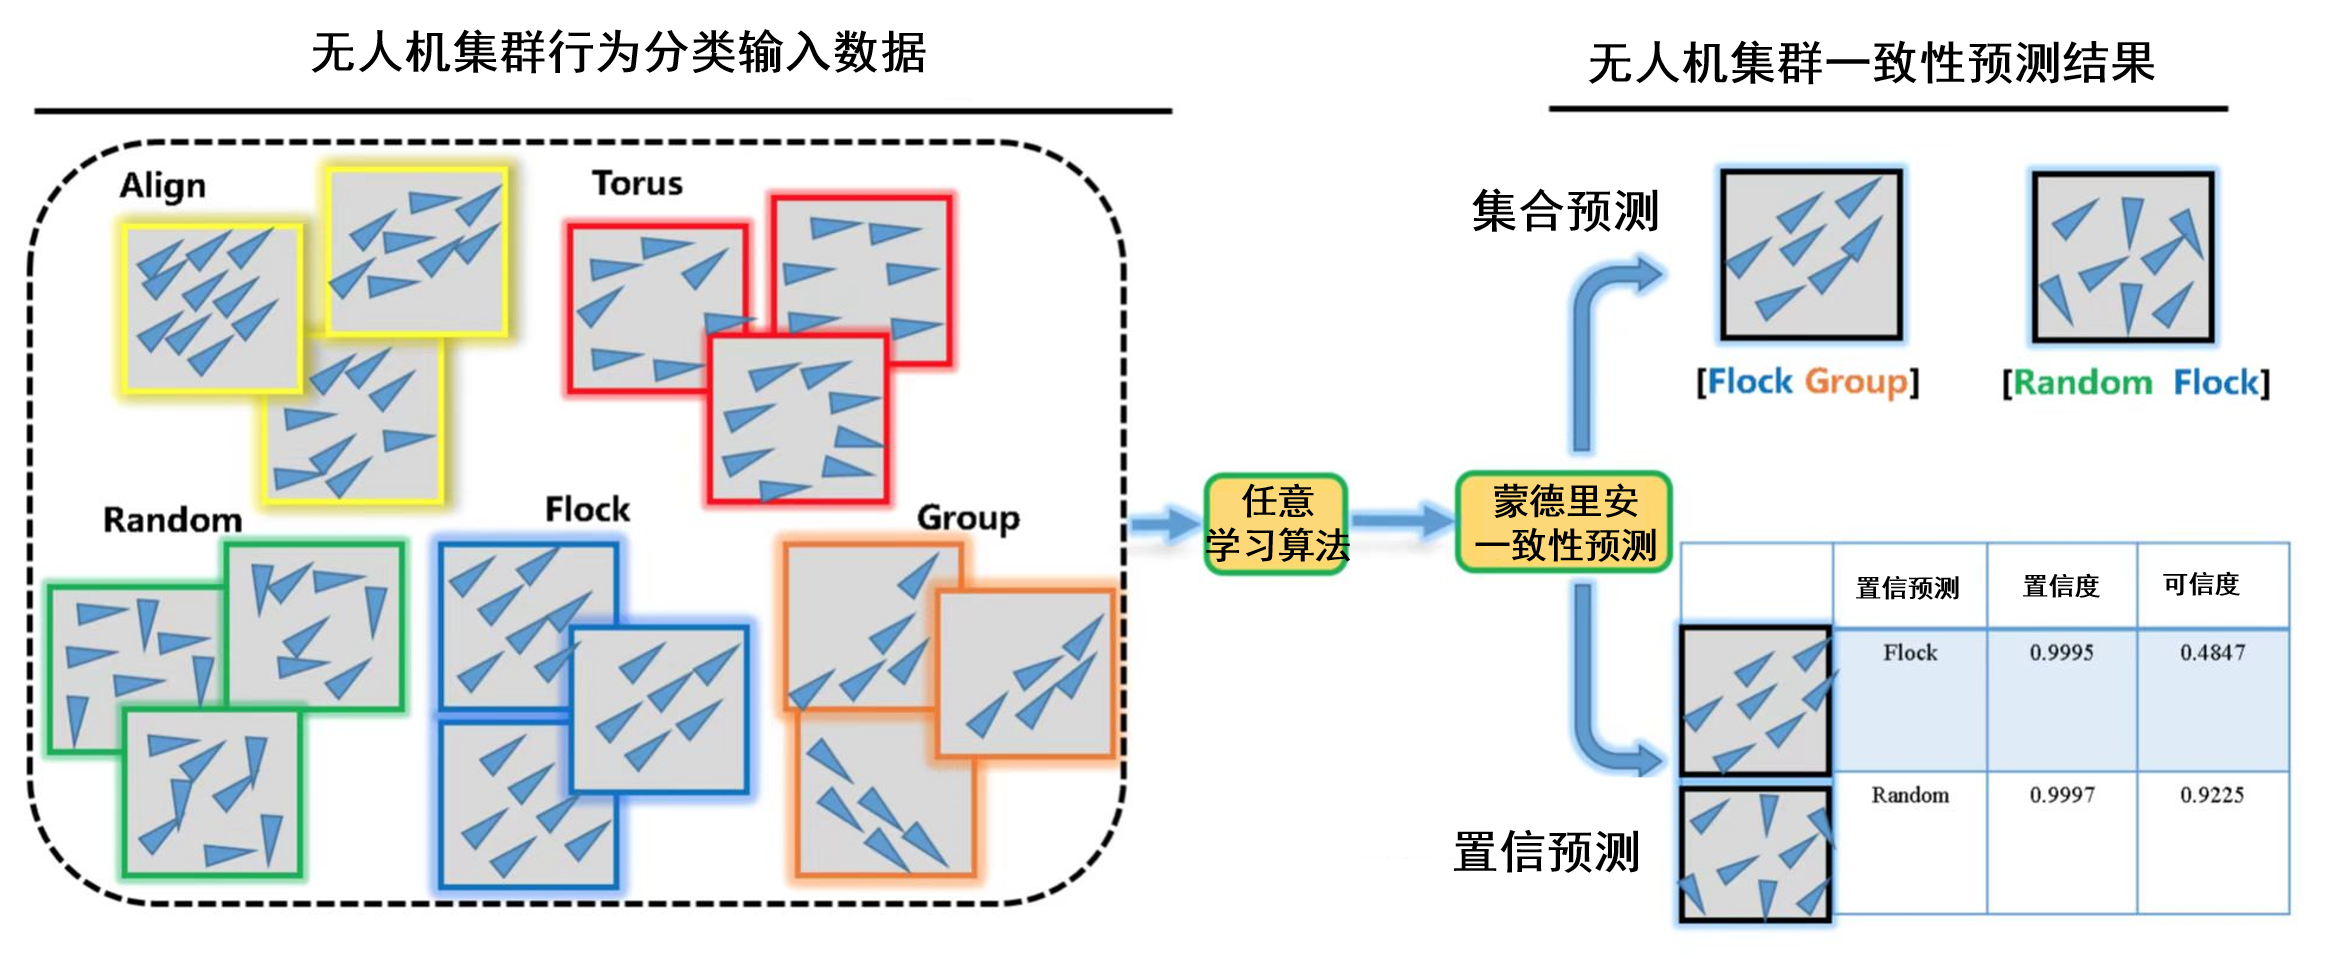
\includegraphics[width=1\linewidth]{Img/chapter8/MCP}
\caption{无人机集群行为分类蒙德里安一致性预测方案框架图}
\label{fig:MCP-framework}
\end{figure}

首先介绍获取无人机集群数据建模, 分别介绍两种集群行为数据集, 即仿真无人机集群数据集(多类别分类问题)和真实无人机集群行为数据集(二元分类问题)。

\subsection{仿真无人机集群行为数据}
\label{sec:dynamic}
对于无人机集群行为的仿真数据, 动力学模型来自于\citet{Flocks1987}。 按照\citet{Thomas2021}给出的\citet{Flocks1987}动力学模型, 有
\begin{align}
F_{ri} &= \sum_{j=1}^{N_{r}}\frac{x_{i} - x_{j}}{||x_{i} - x_{j}||^{2}},\\
F_{ai} &= \sum_{j=1}^{N_{a}}v_{j} - v_{i},\\
F_{hi} &= x_{h_{i}} - x_{i},\\
F_{fi} &= -v_{i}\frac{(||v_{i}|| - s)}{s}.
\end{align}
其中, 这里$N_{r}, N_{a}$分别表示位于排斥力(repulsion)和对齐力(alignment)域内的智能体的数量, $x_{h}$表示中心位置(home location), $r_r$ 和 $r_a$ 分别表示排斥力和对齐力的作用半径, $||\cdot||$ 表示欧式范数。 $x_{i}$ 和 $v_{i}$ 表示位置信息和速度信息。 因此, 动力学模型中智能体所受的合力可表述为下列表达式:
\begin{align}
F_{i}(t) = K_{a}F_{ai} + K_{r}F_{ri} + K_{f}F_{fi} + K_{h}F_{hi},
\end{align}  
其中, 这里的系数$K$确定智能体所受各种力的比例属性。 在动力学模型中, 还为受力模型加入一层非线性过滤函数, 即对于终端的输出, 按照下列表达式
\begin{align}
F_{i}(t) \mapsto \alpha \tanh (\beta F_{i}(t)),
\end{align}
其中, 这里设置不同的$\alpha$和$\beta$系数以产生不同的集群行为。

对于每个智能体, 假设固定的单位质量, 那么系统的更新按照如下表达式完成:
\begin{align}
\ddot{x}_{i}(t) = F_{i}(t).
\end{align}
对于最终的观测数据, 使用下列欧拉积分方程更新位置信息和速度信息:
\begin{align}
v_{i}(t + \Delta t) &= v_{i}(t) + F_{i}(t)\Delta t,\\
x_{i}(t + \Delta t) &= x_{i}(t) + v_{i}(t)\Delta t.  
\end{align}
因此, 根据以上的动力学模型, 通过分配不同的参数配比达到不同集群行为数据的仿真仿真。在仿真模型中, 设置无人机智能体数目为200, 提取位置信息作为学习算法的输入。 

\subsection{真实无人机集群行为数据}
\label{sec:truth-swarm}
本节介绍真实无人机集群行为数据集。 采集的真实行为数据是根据公开发表在UC Irvine 机器学习数据仓库上的数据集 \footnote{\url{https://archive.ics.uci.edu/ml/datasets/Swarm+Behaviour\#}}。 这一数据由澳大利亚新南威尔士大学托管的一个在线调查获得。 此数据包含三种行为数据集, 分别是\texttt{Flock}行为, \texttt{Align}行为和\texttt{Group}行为。 在线调查的数据本身也是基于某无人机集群行为模型, 但是其标签是由参加在线调查的用户标记的, 将这类数据视为是“真实数据”。

对于每一种无人机集群行为数据集, 其包含24016条记录。 这里的数据记录并不是时间序列数据, 而是按照在线收集顺序排列的, 这样的顺序记录在本节不会展开讨论, 但是在下一章节专门会针对数据的到访时间展开讨论。 表\ref{tab:datainfo} 汇总介绍真实集群行为数据集的概要信息, 这些属性包括:
\begin{table}[]
\centering
\caption{无人机集群行为数据各变量的属性信息表}
\label{tab:datainfo}
\begin{tabular}{@{}ll@{}}
\toprule
属性     & 说明                                                 \\ \midrule
(xm, ym)       & 第$m$个智能体的$X-Y$轴位置向量 \\
(xVelm, yVelm) & 第$m$个智能体的$X-Y$轴速度向量     \\
(xAm, yAm)     & 第$m$个智能体的$X-Y$轴对齐向量                      \\
(xSm, ySm)     & 第$m$个智能体的$X-Y$轴分离向量                     \\
(xCm, yCm)     & 第$m$个智能体的$X-Y$轴凝聚向量                       \\
nACm           & 第$m$个智能体处在对齐或凝聚半径内的数目 \\
nSm            & 第$m$个智能体处在分离半径内的智能体数目         \\
Class          & 二元类别                                      \\ \bottomrule
\end{tabular}
\end{table}
\begin{enumerate}
\item \texttt{xm}, \texttt{ym} 表示第$m$个智能体在$X-Y$轴坐标上的位置信息,
\item \texttt{xVelm}, \texttt{yVelm} 表示第$m$个智能体在$X-Y$轴坐标上的速度信息, 
\item \texttt{xAm}, \texttt{yAm} 表示第$m$个智能体在$X-Y$轴坐标上的对齐向量(the alignment vector)的信息, 
\item \texttt{xSm}, \texttt{ySm} 表示第$m$个智能体分离向量(the separation vector)的信息,
\item \texttt{xCm}, \texttt{yCm} 表示第$m$个智能体凝聚向量(the cohesion vector)的信息, 
\item \texttt{nACm}表示处在对齐或凝聚(Alignment/Cohesion)半径内的智能体的数目, 
\item \texttt{nSm} 表示处在分离半径内的智能体数目。
\end{enumerate}
在属性标记中的$m$表示第$m$个智能体, 其中 $m = 1,\ldots,200$, 表示一共200个智能体。 同样的, 对于每个类别的数据集, 其类别标签是二元标签。 例如, 在Align行为数据集中, “1”表示无人机集群属于Align行为, “0”表示不属于Align行为。 在Flocking(或Group)数据集合中, “1”表示无人机集群属于Flocking(或Group)行为, “0”表示不属于Flocking(或Group)行为。 关于这些真实行为数据的其他方面的信息, 例如数据集大小, 划分的训练集大小, 测试集数目等信息列在表\ref{tab:train_test}中。 
\begin{table}[]
\centering
\caption{无人机集群三种典型行为训练样本和测试样本划分表}
\label{tab:train_test}
\begin{tabular}{@{}llll@{}}
\toprule
数据集 & 维数  & 训练样本数 & 测试样本数  \\ \midrule
Align    & 2400 & 12008     & 12008 \\
Flock    & 2400 & 12008     & 12008 \\
Group    & 2400 & 12008     & 12008 \\ \bottomrule
\end{tabular}
\end{table} 

需要注意的是, 并不是将全部无人机集群观测变量输入学习模型。相反仅仅提取位置坐标作为模型的输入。 因此, 学习算法的输入维数是400(仅以$X-Y$轴的坐标作为输入向量)。 最后, 需要强调的是在训练底层Boosting算法时随机地将数据切分为训练集, 校验集和测试集。 

\subsection{试验一:二元无人机集群行为分类研究}
本节给出无人机集群行为分类一致性预测方案设计, 此问题是为二元分类问题提供不确定量化。分别针对无人机集群行为的实际数据和仿真数据展开讨论。 如表\ref{tab:train_test}所示, 首先按照$1:1$将数据划分为训练集和测试集$Z_{test}$, 再将训练集划分为按照$1:1$随机划分为真实训练集$Z_{proper}$, 校正集合$Z_{calibration}$。采用真实训练集$Z_{proper}$训练底层机器学习算法。


针对无人机集群行为真实数据集, 处理的问题归约为二元模式识别问题。首先, 借助真实训练数据集训练Boosting算法并将之作为底层算法实现MCP方法。常规机器学习算法采用汇总指标(例如均方误差)度量模型预测效果, 无法为单个预测样例提供不确定量化。

与常规机器学习研究中使用的汇总指标作为不确定测量评判标准不同的是, 本文着重考虑为每个预测样例提供有效的不确定量化。 换言之, 一旦得到底层算法的输出结果, 要给学习算法简单预测提供有效的不确定量化。 利用MCP方法将暴力得分转变为非一致得分, 进而通过求解 p-值来完成不确定性量化指标的输出。 需要注意的是, 给出的p-值起到至关重要的作用, 并且基于MCP方法得到的p-值是自动精确有效的。根据定义, 将最大p-值所对应的标签记为预测标签, 并将最大p-值定义为预测可信度, 将1减去第二大p-值定义为预测置信度。 

例如, 对于无人机集群中的排列(Align)行为数据集, MCP方法不仅仅提供预测标签, 而且还提供此预测标签所对应的置信度和可信度。 表\ref{tab:simple-prediction}给出MCP方法下针对Align行为数据集Boosting算法的置信预测结果。 对于表\ref{tab:simple-prediction}中的第0号样本, 排列行为(标记为1)和非排列行为(标记为0)对应的p-值分别是{0.001578}和{0.490446}。MCP方法所预测的标签就是最大的p-值所对应的类别——即类别1, MCP预测置信度和可信度就分别是{0.998422}和{0.490446}。 对于第1号样本, 排列行为(标记为1)和非排列行为(标记为0)对应的p-值分别是{0.079073}和{0.008217}。MCP方法所预测的标签就是最大的p-值所对应的类别——即类别0, MCP预测置信度和可信度就分别是{0.991783}和{0.079073}。 其他样例同样可以得到对应的MCP预测结果以及对应的置信度和可信度。
\begin{table}[]
\caption{无人机集群真实数据集的置信预测结果示例表}
\label{tab:simple-prediction}
\centering
\begin{tabular}{lrrrrrr}
\toprule
{示例样本} & \multicolumn{1}{c}{\begin{tabular}[c]{@{}c@{}}非排列行为\\(标记为0)\end{tabular}} &         \multicolumn{1}{c}{\begin{tabular}[c]{@{}c@{}}排列行为\\(标记为1)\end{tabular}} &  \multicolumn{1}{c}{\begin{tabular}[c]{@{}c@{}}真实\\标签\end{tabular}} &  \multicolumn{1}{c}{\begin{tabular}[c]{@{}c@{}}MCP预测\\标签\end{tabular}} &     置信度 &     可信度 \\
\midrule
0 &  0.001578 &  0.490446 &     1 &    1 &  0.998422 &  0.490446 \\
1 &  0.079073 &  0.008217 &     0 &    0 &  0.991783 &  0.079073 \\
2 &  0.821253 &  0.000954 &     0 &    0 &  0.999046 &  0.821253 \\
3 &  0.002549 &  0.250972 &     1 &    1 &  0.997451 &  0.250972 \\
4 &  0.002752 &  0.387290 &     1 &    1 &  0.997248 &  0.387290 \\
$\ldots$ &  {} &  {} &  {} &     {} &     {} &  {}  \\
12003 &  0.873465 &  0.000006 &     0 &    0 &  0.999994 &  0.873465 \\
12004 &  0.645499 &  0.000051 &     0 &    0 &  0.999949 &  0.645499 \\
12005 &  0.476809 &  0.000863 &     0 &    0 &  0.999137 &  0.476809 \\
12006 &  0.702656 &  0.002115 &     0 &    0 &  0.997885 &  0.702656 \\
12007 &  0.062616 &  0.008220 &     1 &    0 &  0.991780 &  0.062616 \\
\bottomrule
\end{tabular}
\end{table}


对于集合预测的情形, 表\ref{tab:set-prediction}给出在显著性水平 $\epsilon = 0, 0.01, 0.05, 0.2, 0.5$ 以及$0.95$ 情形下的集合预测结果。 显著性水平$\epsilon$可以按照下列方式理解, 即在100次随机试验中:
\begin{enumerate}
\item 当设定显著性水平$\epsilon = 0$时: 即要求计算机给出的结果必须全部正确,
\item 当设定显著性水平$\epsilon = 0.01$时: 即要求计算机给出的结果最多错1个,
\item 当设定显著性水平$\epsilon = 0.05$时: 即要求计算机给出的结果最多错5个。
\end{enumerate}
因此, 显著性水平$\epsilon$表征用户对计算机所给出的一种要求。本文将真实标签也在表的最后一列给出, 以便对照MCP是否预测正确。 容易知道, 对于二元分类问题一共有如下三种预测结果, 
\begin{enumerate}
\item 二元素集合预测, 即预测结果为 “$[0,1]$”,
\item 单元素集合预测, 即预测结果为 “$[0]$” 或者 “$[1]$”,
\item 零元素集合预测, 即预测结果为 “$[]$”(表示“空集”)。
\end{enumerate}
\begin{table}[]
\renewcommand{\arraystretch}{1.3}
\caption{无人机集群真实数据集的集合预测结果示例表}
\label{tab:set-prediction}
\centering
\begin{tabular}{lrrllllllr}
\toprule
{示例样本} & \multicolumn{1}{c}{\begin{tabular}[c]{@{}c@{}}非排列行为\\(标记为0)\end{tabular}} &  \multicolumn{1}{c}{\begin{tabular}[c]{@{}c@{}}排列行为\\(标记为1)\end{tabular}} &     0.0 & 0.01 & 0.05 &  0.2 &  0.5 & 0.95 &  \multicolumn{1}{c}{\begin{tabular}[c]{@{}c@{}}真实\\标签\end{tabular}} \\
\midrule
0 &  0.001578 &  0.490446 &  [0, 1] &  [1] &  [1] &  [1] &   [] &   [] &     1 \\
1 &  0.079073 &  0.008217 &  [0, 1] &  [0] &  [0] &   [] &   [] &   [] &     0 \\
2 &  0.821253 &  0.000954 &  [0, 1] &  [0] &  [0] &  [0] &  [0] &   [] &     0 \\
3 &  0.002549 &  0.250972 &  [0, 1] &  [1] &  [1] &  [1] &   [] &   [] &     1 \\
4 &  0.002752 &  0.387290 &  [0, 1] &  [1] &  [1] &  [1] &   [] &   [] &     1 \\
$\ldots$ &  {} &  {} &  {} &     {} &     {} &  {} &     {} & {} & {}\\
12003 &  0.873465 &  0.000006 &  [0, 1] &  [0] &  [0] &  [0] &  [0] &   [] &     0 \\
12004 &  0.645499 &  0.000051 &  [0, 1] &  [0] &  [0] &  [0] &  [0] &   [] &     0 \\
12005 &  0.476809 &  0.000863 &  [0, 1] &  [0] &  [0] &  [0] &   [] &   [] &     0 \\
12006 &  0.702656 &  0.002115 &  [0, 1] &  [0] &  [0] &  [0] &  [0] &   [] &     0 \\
12007 &  0.062616 &  0.008220 &  [0, 1] &  [0] &  [0] &   [] &   [] &   [] &     1 \\
\bottomrule
\end{tabular}
\end{table}

在表\ref{tab:set-prediction}提供的集合预测中, 例如对于第0号样本, 在显著性水平$\epsilon=0.05$下, 得到的集合预测结果是 “$[1]$”(此时的集合预测结果是正确的), 而在显著性水平$\epsilon=0.5$下所得的集合预测结果是 “$[]$”(此时的集合预测结果为“空集”, 是预测错误的)。 对于第1号样本, 在显著性水平$\epsilon=0.05$下, 得到的集合预测结果是 “$[0]$”(此时的集合预测结果是正确的), 而在显著性水平$\epsilon=0.5$下所得的集合预测结果是 “$[]$”(此时的集合预测结果是错误的)。 对于第12006号样本, 在显著性水平$\epsilon=0.05$下, 得到的集合预测结果是 “$[0]$”(此时的集合预测结果是正确的), 而在显著性水平$\epsilon=0.5$下所得的集合预测结果还是“$[0]$”(此时的集合预测结果也是正确的)。 其他样例同样可以得到任意显著性水平下的集合预测结果。

此外, 还通过对比采用蒙德里安一致性预测校正和不校正前后错误率的控制来说明MCP校正的有效性。 图\ref{fig:validity}展示的是每个类别下错误控制采用蒙德里安一致性预测校正前后的比对。图\ref{fig:validity}的上面两幅是校正前两个类别的错误控制, 下图是采用MCP方法校正后的错误控制。从图中可以看到, 在采用MCP算法校正之前, 模型的错误并没有得到有效控制。例如, 对于预测结果为类别0的样本(图\ref{fig:validity}的左上), 在显著性水平低于0.2时, 机器学习算法的错误控制是失效的, 因为经验错误率低于理论要求错误率; 当显著性水平高于0.2时, 机器学习算法的错误控制在理论上亦是失效的, 因为经验错误率高于理论要求显著性水平。对于预测结果为类别1的样本(图\ref{fig:validity}的右上), 很明显机器学习算法的错误控制一直都是失效的, 因为经验错误率始终大于理论要求的显著性水平。然而, 经过MCP算法校正后, 预测结果的错误率都得到有效保证。从图\ref{fig:validity}可知, 经过蒙德里安一致性预测校正后, 无论是类别0的样本还是类别1, 其预测结果的错误控制都得到有效保证。
\begin{figure}[]
\centering
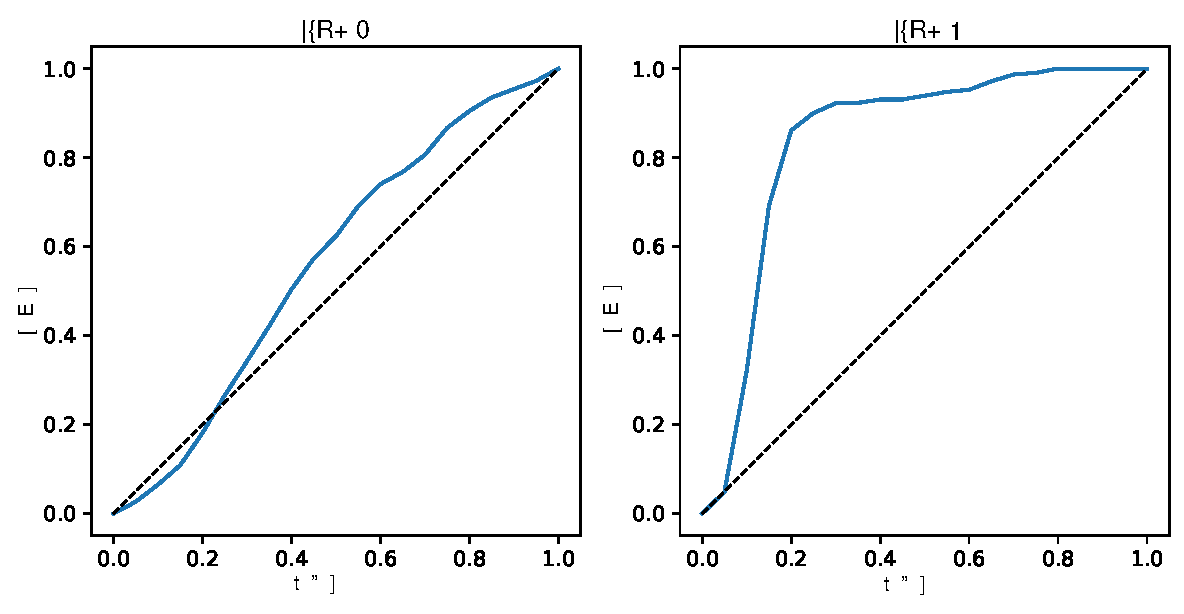
\includegraphics[width=1\linewidth]{Img/chapter8/invalidity}
$$\Downarrow \quad \textsf{经过蒙德里安一致性预测校正} \quad \Downarrow$$
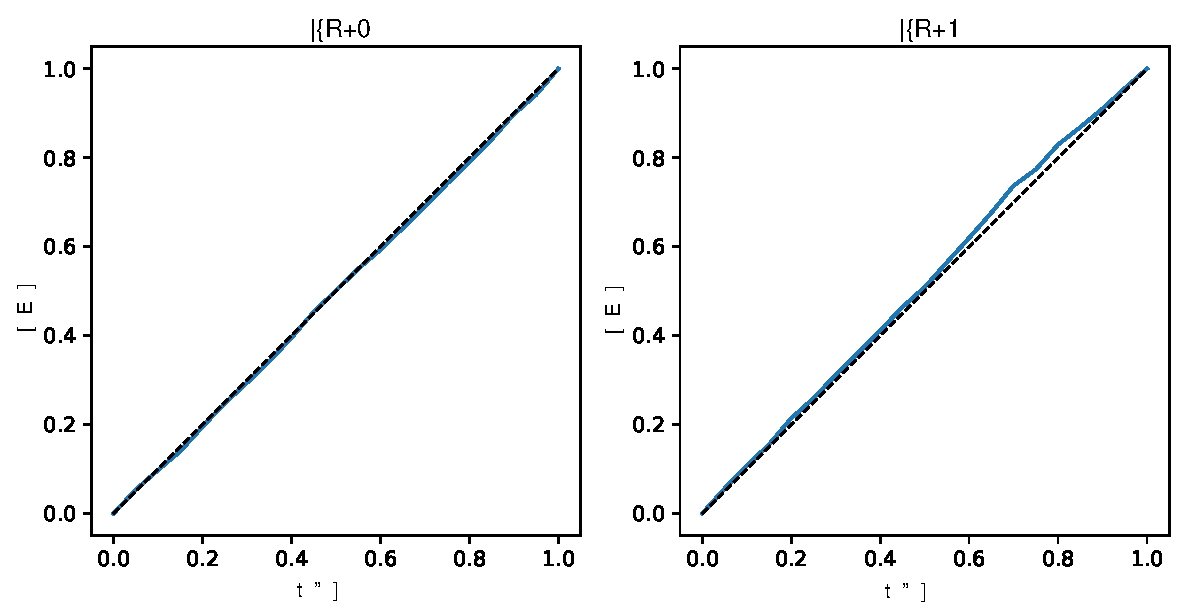
\includegraphics[width=1\linewidth]{Img/chapter8/validity}
\caption{MCP方法校正前后无人机集群真实数据集错误控制对比}
\label{fig:validity}
\end{figure}

\subsection{试验二:多元无人机集群行为分类研究}
针对复杂无人机集群行为分类问题, 在仿真数据上考虑生成多种无人机集群行为, 此问题是为多类别分类问题提供不确定量化。因此, 在无人机集群行为仿真数据集的研究中, 需要处理多类别分类任务。

基于第\ref{sec:dynamic}节所述的无人机集群动力学模型, 仿真三种具有代表性的无人机集群行为, 分别记为排列(Align)行为(标记为0), 聚集(Flock)行为(标记为1)和组队(Group)(标记为2)。 其他无人机集群的个体规模按照表\ref{tab:train_test}设置相同的参数。 同样的, 将仿真数据集按照$1:1:1$比例随机划分为真实训练集$Z_{proper}$, 校正集合$Z_{calibration}$和测试集$Z_{test}$。利用真实训练集$Z_{proper}$训练底层Boosting算法。

表\ref{tab:sys-simple-prediction}列出的是针对无人机集群行为仿真数据集, 蒙德里安一致性预测给出的置信预测结果。 例如, 对于第0号样例, 类别0,1,2对应计算得到的p-值分别是0.41, 0.33和0.26。 根据蒙德里安一致性预测理论其预测标签为0(此样例的蒙德里安一致性预测给出正确预测结果), 此时这种预测结果对应的置信度和可信度分别为0.67和0.41。 对于第1号样例, 类别0,1,2对应计算得到的p-值分别是0.34, 0.44和0.22。 根据蒙德里安一致性预测理论其预测标签为1(此样例的蒙德里安一致性预测给出错误预测结果), 此时这种预测结果对应的置信度和可信度分别为0.66和0.44。 对于第2号样例, 类别0,1,2对应计算得到的p-值分别是0.19, 0.34和0.47。 根据蒙德里安一致性预测理论其预测标签为2(此样例的蒙德里安一致性预测给出正确预测结果), 对应的置信度和可信度分别为0.66和0.47。

\begin{table}[]
\caption{无人机集群仿真数据集的置信预测结果示例表}
\label{tab:sys-simple-prediction}
\centering
\begin{tabular}{lrrrrrrr}
\toprule
\multicolumn{1}{c}{\begin{tabular}[c]{@{}c@{}}示例\\ 样本\end{tabular}} & \multicolumn{1}{c}{\begin{tabular}[c]{@{}c@{}}排列行为\\(标记为0)\end{tabular}} & \multicolumn{1}{c}{\begin{tabular}[c]{@{}c@{}}聚集行为\\(标记为1)\end{tabular}}  & \multicolumn{1}{c}{\begin{tabular}[c]{@{}c@{}}组队行为\\ (标记为2)\end{tabular}}  &  \multicolumn{1}{c}{\begin{tabular}[c]{@{}c@{}}真实\\ 标签\end{tabular}} &  \multicolumn{1}{c}{\begin{tabular}[c]{@{}c@{}}MCP\\ 预测标签\end{tabular}} &  置信度 &  可信度 \\
\midrule
0 &  0.41 &  0.33 &  0.26 &     0 &    0 &   0.67 &   0.41 \\
1 &  0.34 &  0.44 &  0.22 &     2 &    1 &   0.66 &   0.44 \\
2 &  0.19 &  0.34 &  0.47 &     2 &    2 &   0.66 &   0.47 \\
3 &  0.26 &  0.49 &  0.25 &     1 &    1 &   0.74 &   0.49 \\
$\ldots$ &  {} &  {} &  {} &     {} &     {} &  {} &     {} \\
12003 &  0.37 &  0.18 &  0.45 &     2 &    2 &   0.63 &   0.45 \\
12004 &  0.50 &  0.38 &  0.12 &     0 &    0 &   0.62 &   0.50 \\
12005 &  0.52 &  0.30 &  0.18 &     0 &    0 &   0.70 &   0.52 \\
12006 &  0.24 &  0.45 &  0.31 &     1 &    1 &   0.69 &   0.45 \\
12007 &  0.14 &  0.14 &  0.72 &     2 &    2 &   0.86 &   0.72 \\
\bottomrule
\end{tabular}
\end{table}
表\ref{tab:sys-set-prediction}给出的是利用蒙德里安一致性预测算法, 在指定显著性水平取值$\epsilon=0.15, 0.2, 0.4$下的集合预测结果。对于第0号样本, 类别0,1,2对应计算得到的p-值分别是0.41, 0.33和0.26。 根据MCP理论其在显著性水平$\epsilon = 0.15, 0.2, 0.4$ 下的集合预测结果分别是 $[0, 1, 2]$(预测正确), $[0, 1, 2]$(预测正确)和$[0]$(预测正确)。对于第1号样本, 类别0,1,2对应计算得到的p-值分别是0.34, 0.44和0.22。 根据MCP理论其在显著性水平$\epsilon = 0.15, 0.2, 0.4$ 下的集合预测结果分别是 $[0, 1, 2]$(预测正确), $[0, 1, 2]$(预测正确)和$[1]$(预测错误)。对于第2号样本, 类别0,1,2对应计算得到的p-值分别是0.19, 0.34和0.47。 根据MCP理论其在显著性水平$\epsilon = 0.15, 0.2, 0.4$ 下的集合预测结果分别是 $[0, 1, 2]$(预测正确), $[ 1, 2]$(预测正确)和$[2]$(预测正确)。
\begin{table}[]
\caption{无人机集群仿真数据集的集合预测结果示例表}
\label{tab:sys-set-prediction}
\centering
\begin{tabular}{lrrrlllr}
\toprule
\multicolumn{1}{c}{\begin{tabular}[c]{@{}c@{}}示例\\ 样本\end{tabular}} & \multicolumn{1}{c}{\begin{tabular}[c]{@{}c@{}}排列行为\\(标记为0)\end{tabular}} &  \multicolumn{1}{c}{\begin{tabular}[c]{@{}c@{}}聚集行为\\(标记为1)\end{tabular}}  &   \multicolumn{1}{c}{\begin{tabular}[c]{@{}c@{}}组队行为\\(标记为2)\end{tabular}} &       0.15 &        0.2 &  0.4 &  \multicolumn{1}{c}{\begin{tabular}[c]{@{}c@{}}真实\\标签\end{tabular}} \\
\midrule
0 &  0.41 &  0.33 &  0.26 &  [0, 1, 2] &  [0, 1, 2] &  [0] &     0 \\
1 &  0.34 &  0.44 &  0.22 &  [0, 1, 2] &  [0, 1, 2] &  [1] &     2 \\
2 &  0.19 &  0.34 &  0.47 &  [0, 1, 2] &     [1, 2] &  [2] &     2 \\
3 &  0.26 &  0.49 &  0.25 &  [0, 1, 2] &  [0, 1, 2] &  [1] &     1 \\
$\ldots$ &  {} &  {} &  {} &     {} &     {} &  {} &     {} \\
12003 &  0.37 &  0.18 &  0.45 &  [0, 1, 2] &     [0, 2] &  [2] &     2 \\
12004 &  0.50 &  0.38 &  0.12 &     [0, 1] &     [0, 1] &  [0] &     0 \\
12005 &  0.52 &  0.30 &  0.18 &  [0, 1, 2] &     [0, 1] &  [0] &     0 \\
12006 &  0.24 &  0.45 &  0.31 &  [0, 1, 2] &  [0, 1, 2] &  [1] &     1 \\
12007 &  0.14 &  0.14 &  0.72 &        [2] &        [2] &  [2] &     2 \\
\bottomrule
\end{tabular}
\end{table}

同样的, 也针对无人机集群仿真数据集检验经过蒙德里安一致性预测校正后各个类别的错误控制。结果不难发现, 如图\ref{fig:sys-validity}所示, 在采用蒙德里安一致性预测校正之前的机器学习算法对于每个类别的错误控制是失效的, 而经过蒙德里安一致性预测算法校正后每个类别的错误控制都能够和理论要求的错误控制保持一致。
\begin{figure}[]
\centering
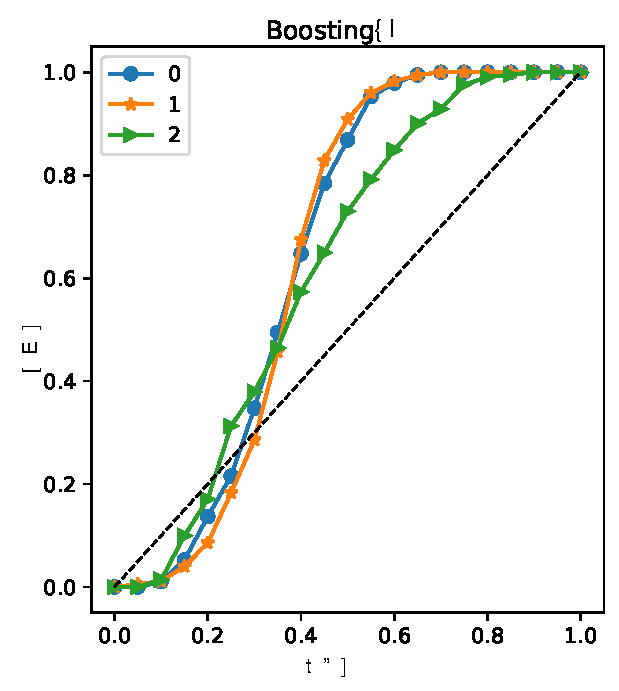
\includegraphics[width=.4\linewidth]{Img/chapter8/boost-invalidity}
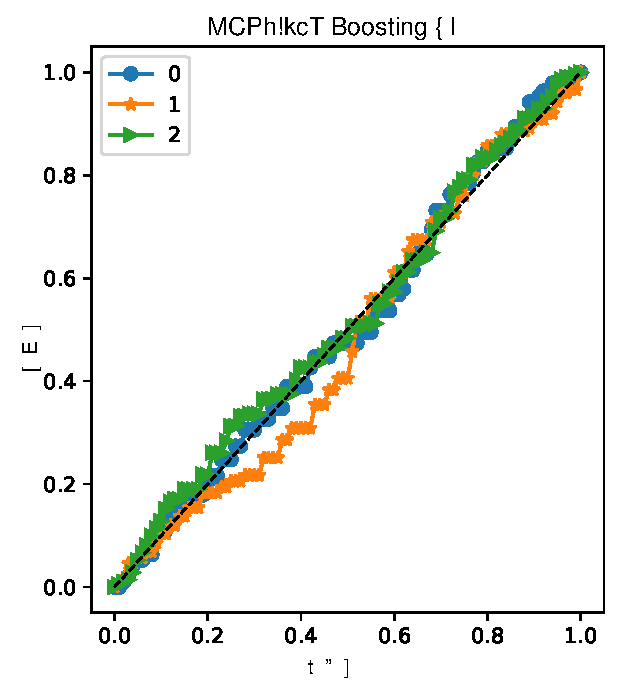
\includegraphics[width=.4\linewidth]{Img/chapter8/boosting-validity}
\caption{MCP方法校正前后无人机集群仿真数据集错误控制对比}
\label{fig:sys-validity}
\end{figure}

\section{本章小结}
\label{sec:discussion}
本章将Boosting算法作为底层机器学习算法, 利用一致性预测理论为无人机集群行为分类提供不确定量化。主要结论总结如下:
\begin{enumerate}
\item 针对二元无人机集群行为真实数据和多元无人机集群仿真数据, 提出采用一致性预测方案为机器学习分类算法输出结果提供无分布假设的不确定量化, 给出置信预测模式。试验数据表明, 一致性预测理论给出置信预测模式的有效性是自动满足的;
\item 针对二元无人机集群行为真实数据和多元无人机集群仿真数据, 提出采用一致性预测方案给出集合预测模式。试验数据表明, 集合预测能够实现在任意显著性水平下有保证的多类别预测结果;
\item 检验经过一致性预测校正前后各个类别的错误控制。试验数据表明, 未经一致性预测理论校正的常规机器学习算法无法达到有效错误控制; 经过一致性预测方法校正后, 每个类别的错误控制都得到有效控制, 使得理论误差和实际误差保持一致。
\end{enumerate}

\chapter{无人机集群行为数据的分布漂移检测方法研究}
\label{chapter:swarm-distributions}

\section{引言}
\label{Introduction}
根据第\ref{chap:edbed}章关于机器学习一致收敛的理论分析可知, 机器学习算法的基本前提假设是经验数据由固定的、但是未知的分布独立地生成\citep{vapnik1995, vapnik1998, Vapnik2006}。 在具体实际应用中, 研究者通常会将得到的数据集随机采样为训练集和测试集。根据Bruno de Finetti(1906-1985)提出的现代概率论批判理论\citep{Finetti1975}, 将经验数据利用现代计算技术随机处理后能使得经验数据满足概率论理论要求, 但同时也将经验数据本身的分布信息忽视\citep{shiryaev2016-1,shiryaev2016-2}。

在开展有关无人机集群行为分类任务的实际工程应用中, 需要按照无人机集群行为数据本身的时间顺序构建模型。如果在构建模型前将数据随机采样为训练集和测试集, 构建的机器学习模型的泛化推广能力将会产生相当优越的预测性能, 但是如果按照数据本身原有的时间顺序划分训练集和测试集, 构建的机器学习模型相较于随机化后的机器学习模型的泛化推广能力会产生巨大的偏差\citep{Shafer2022}。针对此问题有效的解决办法之一是通过构造一种分布漂移检测算法, 此算法能够检测按照数据本身时间顺序所构建机器学习模型泛化推广能力的边界, 从而对机器学习算法的预测能力提前给出预警。因此, 关于分布漂移检测技术建模是处理实际工程应用中的关键技术之一, 值得对此展开重点研究。

无人机集群行为数据是一个典型的超高维变量映射问题, 而传统统计学给出的关于分布漂移检测的相关理论(如变点检测\citep{Wang2021},协方差漂移\citep{Kpotufe2021})均存在“维数灾难”的技术瓶颈\citep{Alexey2013,Shafer2022}, 并且传统统计学将“检测分布漂移”技术性地归约为“检测假设的分布漂移”\citep{Fisher1956,CDenis1990,Malyutov2018}。因此, 在传统统计学建制下给出的理论无法满足实际工程应用的需要。然而, 有关无人机集群行为问题的实际工程应用研究的现实需要则直接要求研究者解决如下两个问题, 一方面必须研究适用于超高维问题的分布漂移检测问题\citep{Vapnik2006}, 另一方面必须研究检测数据本身的分布漂移问题\citep{2003Universal}。


\section{基于一致性预测的分布漂移检测研究}
\label{sec:martingales}
本文提出的无分布假设的分布漂移检测方法为这实际工程应用提供一种端到端的解决方案, 此算法思想来源于Vovk提出的一般经验概率理论\citep{Vovk1993}。 \citet{Vovk1993}提出采用鞅理论方法补充Kolmogorov概率论\citep{Kolmogorov1933,Kolmogorov-en-1956,Kolmogorov-en-1946-leastsquare}中无法解决的零概率测度问题\citep{Shafer2018,Bienvenu2022}, 并且将鞅方法扩展至处理分布漂移检测问题\citep{Vovk2003}。通常而言, 考虑数据本身时间顺序的有序预测将分布漂移检测方法归约为在一致性预测框架内开展零概率测度问题\citep{gammerman1998}。如图\ref{fig:martingale}所示, 该图展示所提方法的总体框架。从该框架图可知, 该算法主要分为三个过程, 即数据准备、底层机器学习算法构建和分布漂移检测。其中, 在分布漂移检测环节, 需要按照一致性预测理论计算p-值, 进而得到检测分布漂移的鞅序列。所有的计算流程都可建立在机器学习算法顶层。

\begin{figure*}[htbp] % [tb]
\centerline{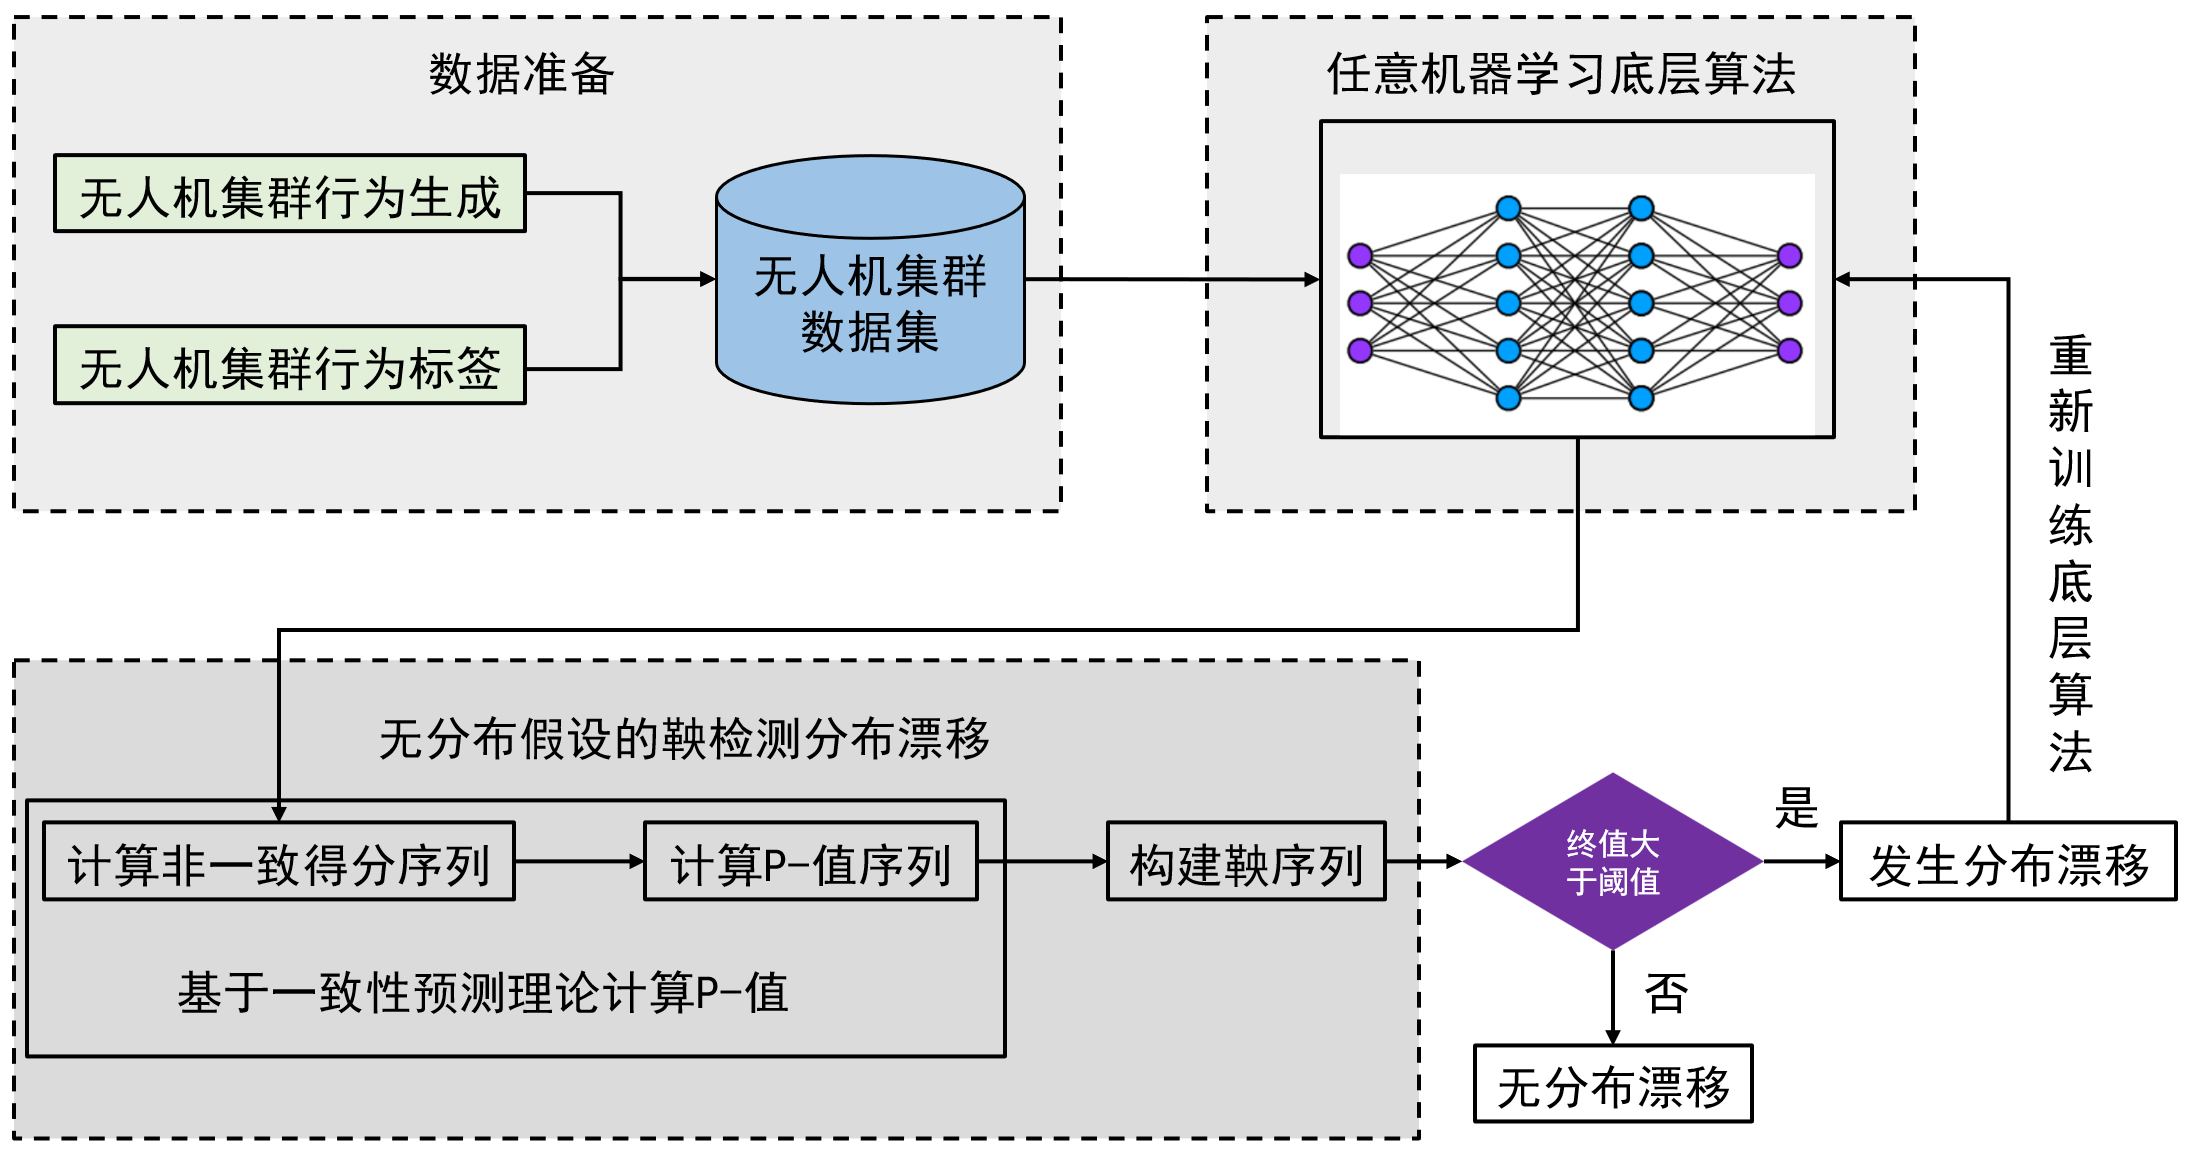
\includegraphics[width=1\linewidth]{Img/martingale.png}}
\caption{无分布假设鞅序列分布漂移检测方案框架图}
\label{fig:martingale}
\end{figure*}

本文针对真实无人机集群行为数据展开分布漂移检测。因此在数据准确阶段直接采用第\ref{chap:Swarm-MCP}章中的公开无人机集群行为数据集作为研究对象, 并且在构建底层机器学习算法时严格按照数据本身的时间顺序将无人机集群数据划分为训练集和测试集。使用训练集得到学习模型后, 便可以利用此学习模型得到测试数据集的预测结果, 然后根据机器学习预测输出结果构建分布漂移检测方法。

本文提出的分布漂移检测方法是建立在机器学习模型之上的, 因此, 可以选取任意的机器学习模型作为底层算法。选择三种具有代表性的现代机器学习算法, 分别是全连接神经网络算法,Boosting算法和支持向量机算法。根据训练数据得到机器学习算法的参数设定后, 底层机器学习算法被视为超越算子, 因此测试数据经过超越算子后被压缩为单个值, 本文提出的分布漂移检测算法就是基于此压缩值而展开分析的。

在第\ref{chap:edbed}章和第\ref{chap:Swarm-MCP}章中已经阐明, 机器学习算法的输出结果仅仅表征样本之间的相似度\citep{vapniktalk2022}, 因此需要利用一致性预测理论计算其对应的非一致性得分。进而根据通过一致性预测得到经验数据对应的p-值序列\citep{2006Hedging}, 然后基于计算得到的p-值序列构建权力鞅(power martingales)序列\citep{Ville1939}。权力鞅序列的构建无需任何分布假设, 因此称之为无分布假设的鞅序列检测分布漂移方法(Distributions-free Martingales Test Distributions-shift)。 

基于已有的鞅理论\citep{glenn-vovk2001,glenn-vovk2019}, 所构建的权力鞅序列能够实现分布漂移检测的任务。根据鞅理论的研究成果, 本文提出一旦权力鞅序列的取值超过某个提前给定的阈值(此阈值根据鞅理论, 取值一般在20-100之间。本文将此阈值设定在最宽松情形下, 即阈值设定为100), 就认为此时的底层机器学习算法对后续测试数据无法提供高效的预测, 认定此时数据发生分布漂移。

然而, 尽最大努力调研文献之后发现很少有研究关注到当利用机器学习算法处理真实无人机集群行为预测时, 考虑对无人机集群行为数据本身分布漂移的检测研究。即很少有研究关注到如何对机器学习模型的条件假设给出检测的问题。 这就是说, 利用机器学习算法确实能够实现真实数据的分类, 这些优良的分类结果大都建立在默认将数据随机采样得到训练集和测试集, 然后利用训练集得到预测模型, 进而在测试数据集上展开预测分析。

但本章考虑的问题是: 如果不进行随机采样, 严格按照实际工程数据的真实顺序划分训练集和数据集。在不随机采样数据的要求下, 利用训练集训练模型, 并在测试集上检验模型的预测能力。在这种情形下就需要检测所得机器学习模型是否会继续保持优质的预测能力。如果随机采样数据不会对机器学习算法预测能力产生较大影响, 那么真实数据没有发生分布漂移, 因此研究者可以继续使用先前训练模型为后续测试样本提供预测。如果对比随机采样数据前后机器学习模型预测能力有较大差距, 这说明数据本身的时间顺序是值得被关注的研究对象, 因此分布漂移检测就能够为机器学习算法预测能力提供一种预警。  

就文献调研所知, 第一个针对实际数据展开分布漂移的研究是由\citet{Vovk2003}在考虑USPS手写数字问题中提出的。 \citet{Vovk2003}考虑针对美国国家邮政局(U.S. Postal Service, USPS)提供的手写数字识别展开研究。 此数据集一共包含9298个16$\times$16像素灰度的手写数字, 此数据集保留美国国家邮政局收集数据时的时间顺序\citep{vovk-pvalue2019}。 Vovk将自己提出的鞅方法应用到原初USPS数据集上发现, 机器学习对于随机化数据和按照真实数据顺序这两种情形的学习推广能力有巨大的差别。

根据Bruno de Finetti现代概率论批判理论可知\citep{Finetti1975}, 分布漂移检测问题更一般的理论陈述是“随机变量可交换性检测”问题\citep{Finetti1975}。\citet{Vovk2003}提出使用鞅序列方法检测随机变量的可交换性并且指出对于实际工程问题, 数据的可交换性假设通常是被拒绝的, 即对于实际工程应用中的真实数据, 是不满足可交换性假设的。换言之, Bruno de Finetti现代概率论批判理论指出, 在自然科学研究中应该严格按照数据本身的顺序展开模型构建, 而不应该将数据随机化操作后再构建学习模型。 

受此启发, 在研究无人机集群行为分类这一实际应用工程问题时也探讨随机化无人机集群行为数据带来的影响。 经过文献调研后发现, 在无人机集群行为分类研究中, 鲜有文献对这一问题展开研究, 然而在其他应用研究领域, 已经有学者应用鞅理论处理实际工程应用。 例如, \citet{Ho2005} 将权力鞅序列理论应用于时变流的变点检测问题上, 并且指出对于任意的机器学习算法, 权力鞅序列给出的分布漂移检测结果能够灵敏检测数据分布的变化, 为时变流工程应用提供切实可信的数据支撑。\citet{Ho2012} 也在变点检测理论中提出可交换性检测的概念, 他的研究结果表明在变点检测问题中, 基于鞅序列的检测方法能够精确给出研制问题的解, 并且可以针对超高维数据展开精确有效的变点检测。 \citet{Ho2019}将鞅序列检测理论成功地应用于飞行器行为的异常检测项目。这些研究表明对于实际工程应用研究, 鞅方法能够为研制问题提供端到端的解决方案。因此, 提出为无人机集群实际工程数据也开展分布漂移检测。

\section{基于一致性预测的鞅序列构建}

本节首先对基于鞅方法的分布漂移检测理论进行介绍。分布漂移检测是可交换性检测的一个特例, 因此, 在Bruno de Finetti现代概率论批判意义下很容易获得分布漂移检测方案。 考虑给定随机变量序列$(Z_1,Z_2,\ldots)$, 其对应的具体输出元素成为样例序列$(z_1, z_2,\ldots)$, 其中每个样例都由两部分组成, 即对象$x_i$和对应的标签$y_i$。 给定原假设: 样例序列$(z_1, z_2, \ldots)$都是根据某个固定的且未知的概率分布函数$P(x)$生成, 即
\begin{center}
\textsf{原假设 $H_0$}: 样例序列没有发生分布漂移。
\end{center}

提出的分布漂移检测方法分为三步完成。 首先根据训练数据训练底层机器学习算法, 按照实际数据本身的时间顺序将数据划分为训练集和测试集。得到底层机器学习算法后, 计算测试数据的预测输出得分。根据第\ref{chap:edbed}章和第\ref{chap:Swarm-MCP}章的阐述可知, 机器学习算法的输出结果仅仅是样本相似程度的度量, 并且只有经过一致性预测算法校正后才能够有效控制错误误差。因此, 第二步需要根据机器学习算法预测输出计算非一致性得分, 进而得到每个样本对应的p-值得分函数。第三步, 根据p-值得分函数结合鞅理论可以构建权力鞅序列。根据鞅理论的研究成果, 权力鞅序列的最终取值不可能过大, 如果权力鞅序列的最终取值超过给定的阈值, 就可以依概率拒绝零假设, 即判定样例序列可能发生分布漂移。

\subsection{基于一致性预测算法计算p-值}
设样例$(z_1,z_2,\ldots)$按照原始顺序依次收集, 根据第\ref{chap:Swarm-MCP}章介绍的一致性预测理论知识, 首先借助底层机器学习算法得到每个样本的预测输出。由于机器学习算法的预测输出仅仅是相似度度量, 需要将每个相似度度量函数按照一致性预测理论计算非一致性得分。一致性预测扮演的角色是将底层机器学习输出的未校正相似度度量函数校正为有效相似程度度量函数。 非一致性得分函数定义为
\begin{align}
\label{alpha-4.1}
\alpha_{i} = A_{n}(\{z_1,\ldots,z_{i-1},z_{i+1},\ldots,z_{n}\}, z_{i}),
\end{align}

根据\citet{vapnik1995,vapnik1998}提出的超越推理理论, 机器学习算法将经验事实以超越推理范式映射至函数的值。因此, 可以选择任意的机器学习算法作为底层超越算子。采用三种经典学习模型作为底层机器学习算法(分别是SVMs, Boosting算法和神经网络算法)计算非一致性得分。

具体而言, 非一致性得分函数的定义可以有众多不同的方法, 中选择逆概率作为非一致性测度函数\citep{Johansson2017}, 即
\begin{align}
\label{alpha-4.2}
\alpha_{i} = - \hat{p}_{i}.
\end{align}
其中, $\hat{p}_{i}$是底层机器学习算法输出的“概率值”。

根据计算得到的非一致得分函数可以快速构建p-值函数序列\citep{vovk2005algorithmic}。通常而言, 可以通过标准化非一致得分来计算p-值函数序列, 即对于样本$z_n$所对应的p-值序列, 按照下列表达式计算可以得到有效的p-值序列
\begin{align}
\label{alpha-4.3}
p_n = \frac{\#\{i: \alpha_i > \alpha_n\} + \tau_n \# \{i: \alpha_i = \alpha_n\}}{n}.
\end{align}
其中, 这里$\tau_n$是随机化因子, 其服从于$[0, 1]$上的均匀分布, 符号 \# 表示集合大小的测度。 显而易见对于任意的底层算法, 根据上述一致性预测方法计算得到的p-值函数是精确有效的, 即根据这种方法计算得到的p-值序列严格服从$[0,1]$上的均匀分布。关于这一陈述的证明参见定理\ref{theorem}, \citet{vovk2005algorithmic}给出关于此定理的证明。

\begin{theorem}
\label{theorem}
如果样例$(z_1,z_2,\ldots)$满足可交换性假设, 那么p-值序列都是独立的并且服从$[0,1]$上的均匀分布。
\end{theorem}
p-值序列精确有效的性质是非常重要的, 因为从统计学理论的要求来看, 借助一致性预测方法生成的精确有效p-值序列为后续展开有效的统计推断提供严格的理论保证。

\subsection{基于p-值构建鞅序列}
\label{sec:aglorithm}
本节详细介绍基于一致性预测校正后有效p-值序列构建鞅方法检测分布漂移。首先, 基于鞅理论设定博弈函数(betting function), 此函数满足鞅理论要求。利用博弈函数的映射关系可以得到每个p-值序列对应的博弈函数取值。权力鞅序列定义为博弈函数取值的乘积。由于给定的博弈函数满足$[0, 1]$上的积分为1, 所以构建得到的权力鞅序列可以视为分布漂移的量化标识。根据鞅理论要求, 如果没有发生分布漂移, 权力鞅序列的取值会一直衰减。换言之, 如果没有发生分布漂移, 权力鞅不会取得较大的值。因此, 仅仅根据权力鞅最终的取值大小即可做出是否拒绝零假设的判断。

具体而言, 对于每个样例$i \in \{1,2,\ldots\}$, 设下列函数
\begin{align}
f_i : [0,1]^{i} \rightarrow [0, \infty)
\end{align}
是给定的博弈函数, 此函数将服从$[0,1]$上的均匀分布随机变量映射至非负取值变量, 并且定义函数满足下列表达式,
\begin{align}
\label{betting}
\forall i: f(p_i) = \varepsilon p_{i}^{\varepsilon -1}.
\end{align}
其中, 这里$\varepsilon \in [0,1]$。对于博弈函数$f(x)$, 要求满足下列表达式
\begin{align}
\int_{0}^{1}f(x)dx=1.
\end{align}
根据博弈函数, 满足下列表达式的随机序列定义为权力鞅序列, 
\begin{align}
M_{n}^{(\varepsilon)} := \prod_{i=1}^{n}(\varepsilon p_{i}^{\varepsilon - 1}),
\end{align}
其中, 这里的 $p_1, p_2, \ldots, p_n$是借助一致性预测方法计算得到的p-值序列, 此序列是以初始值为1的非负的、被随机化后的鞅序列。 这一类鞅序列称为随机化的权力鞅序列(randomised power martingales), 简称权力鞅序列。

根据鞅理论\citep{Ville1939,Doob1984}, 满足零假设的鞅序列满足下列表达式
\begin{align}
\label{alpha-4.7}
M_{n} \geq E(M_{n+1} | \mathcal{F}_{n}),
\end{align}
其中, 这里$\mathcal{F}_{n}$是由序列$z_{1}, \ldots, z_{n}$生成的$\sigma$-代数。如果$M_{0}=1$并且$\inf_{n}M_{n} \geq 0$, 那么随机过程$M_{0}, M_{1}, \ldots$被定义为资本过程\citep{Vovk1993,vovk2001,vovk2021,Bienvenu2022,Laurent2009,Bienvenu2009OnTH}。“资本过程”这一术语形象地阐述分布漂移检测理论的思想, 即按照鞅理论此资本过程表示赌徒从单位资产出发, 每次都押注: “按照公平的自然选择, 所得的结果$M_{n}$并不会使自己破产”。按照鞅理论来理解学习过程, 即每次都押注: “按照机器给出的结果预测测试样本, 那么测试样本对应的预测结果在总体上不会大面积出错”。所以测试样本对应的权力鞅序列$M_{n}$就不可能取得一个较大的值。这就表明, 依靠训练数据得到的机器学习模型仍然能够为测试数据提供预测, 即测试数据的分布没有发生漂移。

根据鞅理论\citep{Ville1939,Doob1984}, 满足零假设的鞅序列满足下列表达式
\begin{align}
\label{martingale-C}
P\{\forall n: M_{n} \geq C\} \leq \frac{1}{C},
\end{align}
其中, $C$是任意取值为正的常数。 此条件表明, 当数据没有发生分布漂移时, 鞅序列不会取得较大的值。因此, 在分布漂移检测方法中, 如果数据对应的鞅序列取得较大值, 那么就可以依概率拒绝零假设, 认为发生分布漂移。算法 \ref{alg:on-line-testing} 给出整个无分布假设鞅实现分布漂移的检测算法(Distributions-free Martingale Test Distributions-shift, DFMTDS)。

\begin{algorithm}[!htbp]
    \small
    \caption{无分布假设的鞅检测分布漂移算法(DFMTDS)}
    \label{alg:on-line-testing}
    \hspace*{\algorithmicindent} \textbf{输入:} {$z_{i}, i=1,\ldots,n$, 底层算法$T$, $\epsilon$.}\\
    \hspace*{\algorithmicindent} \textbf{输出:} {鞅序列的终值$M_{n}$.}
    \begin{algorithmic}[1]
        \Procedure{DFMTDS}{}
        \State 利用训练数据集训练学习模型$T$,
        \For{$i=1$ {\bfseries to} $n$}
        \State 使用表达式(\ref{alpha-4.2})计算 $\alpha_i$,
        \State 使用表达式(\ref{alpha-4.3})计算 $p_i$,
        \State 使用表达式(\ref{alpha-4.7})计算 $M_{i}$,
        \EndFor
        \While{$M_{n} \leq \epsilon$}
        \State 根据表达式(\ref{martingale-C})返回 $M_{n}$.
        \EndWhile
        \EndProcedure
    \end{algorithmic}
\end{algorithm}

\section{基于鞅序列的无人机集群数据分布漂移检测}
\label{empiricaldtudies}
本节详细介绍针对无人机集群行为数据的分布漂移检测。对比随机采样无人机集群行为数据和按照无人机集群行为数据本身时间顺序这两种模式下的分布漂移检测。首先介绍本章测试算例所用到的数据集并且对比随机化采样数据前后训练所得机器学习模型的预测能力; 然后按照提出的鞅方法计算在保留无人机集群行为数据本身时间顺序建模情形下, 计算鞅序列的取值; 最后按照提出的鞅方法计算随机化处理无人机集群行为数据的鞅序列。

将无人机集群行为分布漂移检测算法应用于三种公开的真实无人机集群行为数据进行检测。无人机集群行为数据的分布漂移可以通过对比随机化数据前后机器学习算法的鞅序列取值来检测。如果无人机集群行为数据没有发生分布漂移, 那么随机化数据并不会对机器学习的预测效果产生影响,对应的鞅序列取值不会大于给定的阈值。

分别针对三种无人机集群行为真实数据(即Align行为数据集, Flock行为数据集和Group行为数据集)开展分布漂移检测问题。 提供三种机器学习算法作为底层算法并且通过对比三种机器学习算法对应的权力鞅序列的取值实现分布漂移检测。

无人机集群行为数据集已经在第\ref{chap:Swarm-MCP}章已经介绍过, 本章将数据集合划分为6004个训练样本, 剩余的18011个样本作为测试样本。 需要特别注意的是, 本章默认按照保留数据本身的时间顺序划分训练集和测试集。 如第\ref{chap:Swarm-MCP}章所述, 每个样本的属性描述在第\ref{chap:Swarm-MCP}章的表\ref{tab:datainfo}中列出, 本章所用到的数据划分方式在表\ref{tab:train_test1}中给出, 本章仍然仅选择位置坐标作为输入变量。

% Please add the following required packages to your document preamble:
% \usepackage{booktabs}
\begin{table}[]
\centering
\caption{无人机集群三种典型行为训练集和测试集信息汇总表}
\label{tab:train_test1}
\begin{tabular}{@{}llll@{}}
\toprule
数据集 & 维数  & 训练样本数 & 测试样本数  \\ \midrule
Align    & 2400 & 6004     & 18011 \\
Flock    & 2400 & 6004     & 18011 \\
Group    & 2400 & 6004     & 18011 \\ \bottomrule
\end{tabular}
\end{table}

\subsection{随机处理数据前后对比研究}

在开展分布漂移检测之前, 首先对比按照数据本身时间顺序建模和随机化数据建模情形下, 机器学习算法的预测能力。按照表\ref{tab:train_test1}要求下划分训练数据和测试数据。使用前6004个样本训练三种机器学习算法, 然后使用机器学习算法预测后18011个测试样例。表\ref{tab:online}展示有序学习模式下错误分类的数目。从表\ref{tab:online}可以看到, 对于Align行为数据集, 全连接神经网络算法(MLP)预测错误的数目最小; 对于Flock行为数据集, Boosting算法预测错误的数目最小; 对于Group行为数据集, Boosting算法预测错误的数目最小。纵观表\ref{tab:online}中预测错误数目, 发现在保持数据本身时间顺序后, 这三种机器学习算法都并没有表现出极其优越的预测效果。

% Please add the following required packages to your document preamble:
% \usepackage{booktabs}
% \usepackage{graphicx}
\begin{table}[]
\centering
\caption{无人机集群有序学习的预测错误数目汇总表}
\label{tab:online}
\begin{tabular}{@{}llll@{}}
\toprule
数据集   & SVMs预测错误数目 & MLP预测错误数目 & Boosting预测错误数目 \\ \midrule
Align & 1492       & 848       & 1763           \\
Flock & 2928       & 2125      & 2055           \\
Group & 1385       & 1031      & 452            \\ \bottomrule
\end{tabular}%
\end{table}


然而, 如果仅仅在构建模型之前将真实无人机集群行为数据随机处理, 然后再同样按照表\ref{tab:train_test1}中要求划分训练集和测试集。仍然利用训练集得到三种机器学习算法, 两种情形所用的三种底层机器学习算法均采用默认参数。在这种情形下, 与上述唯一不同之处就在于在开展划分训练集和测试集之前, 对数据先行进行随机化处理。 表\ref{tab:offline}展示随机化后三种机器学习算法在三种随机化处理后的无人机集群行为数据集上的预测效果。很明显, 当随机化处理数据后, 三种机器学习算法对于三种无人机集群行为数据都给出相当优越的预测效果。

% Please add the following required packages to your document preamble:
% \usepackage{booktabs}
% \usepackage{graphicx}
\begin{table}[]
\centering
\caption{无人机集群随机化后学习的预测错误数目汇总表}
\label{tab:offline}
\begin{tabular}{@{}llll@{}}
\toprule
数据集   & SVMs预测错误数目 & MLP预测错误数目 & Boosting预测错误数目 \\ \midrule
Align & 1          & 0         & 1              \\
Flock & 0          & 2         & 1              \\
Group & 1          & 2         & 1              \\ \bottomrule
\end{tabular}%
\end{table}


具体而言, 对于Align数据集, 随机化处理前SVMs算法预测错误数目是1492, 随机化后预测错误数目是1; 随机化处理前全连接神经网络算法预测错误数目是848, 随机化后预测错误数目是0; 随机化处理前Boosting算法预测错误数目是1763, 随机化后预测错误数目是1。对于Flock数据集, 随机化处理前SVMs算法预测错误数目是2918, 随机化后预测错误数目是0; 随机化处理前全连接神经网络算法预测错误数目是2125, 随机化后预测错误数目是2; 随机化处理前Boosting算法预测错误数目是2055, 随机化后预测错误数目是1。对于Group数据集, 随机化处理前SVMs算法预测错误数目是1385, 随机化后预测错误数目是1; 随机化处理前全连接神经网络算法预测错误数目是1031, 随机化后预测错误数目是2; 随机化处理前Boosting算法预测错误数目是452, 随机化后预测错误数目是1。

显而易见, 对于实际工程中的无人机集群数据集, 随机化处理数据前后机器学习算法的预测能力具有数量级层面的差距。这一方面说明对于实际数据, 可以通过采用随机化处理数据来实现更高精度的预测, 但是同时也说明, 如果需要按照实际工程数据自身时间顺序建模(例如在实际工程中遇到有序学习任务时, 无法提供随机化真实数据的条件), 那么对于实际数据需要额外关注机器学习算法预测能力的边界。因为随着实际数据本身时间顺序的积累, 数据本身的分布是研究者不得不考虑的重要信息。正因为注意到随机化前后机器学习算法的预测能力所表现的这种巨大差距, 提出对真实无人机集群数据展开分布漂移检测。

\subsection{无人机集群行为数据分布漂移检测}
本节研究利用无分布假设的鞅方法检测无人机集群数据的分布漂移, 以验证对于实际工程中真实无人机集群数据, 所提方法能够高效地指示出分布发生变化的位点。这种方法能够为研究者提供一种提示信息, 即当鞅序列的终值大于给定阈值时, 表明利用先前训练数据得到的机器学习算法已经无法为分布发生变化的测试数据继续提供高效准确的预测, 应该在此时重新训练模型, 以获得更高效的预测性能。根据鞅序列理论, 表达式(\ref{martingale-C})中常数$C$的取值一般选取为$[20, 100]$, 选择最宽松的情形, 即$C=100$。也就是说, 在最宽松的要求下检测真实无人机集群数据是否会有分布漂移的发生。

首先, 对于Align数据集, 图\ref{fig:align-mar}展示三种机器学习算法计算得到的鞅序列。图\ref{fig:align-mar}展示学习样本按照原始顺序进入模型后权力鞅序列的增长情形。 例如, 当采用全连接神经网络作为底层算法时(图示中的“MLP”表示全连接神经网络算法), 权力鞅序列最终的取值大约是$114$, 权力鞅的最终值大于给定的阈值100。对于SVMs算法和Boosting 算法, 其最终的取值分别大约是$246$和$267$, 这两个取值是远远大于给定的阈值100。 这说明对于无人机集群行为数据集, 如果按照数据本身时间顺序建模, 那么在训练集上得到的机器学习算法其泛化推广能力是有边界的。换言之, 大概第14000个样本左右(此时权力鞅的取值达到阈值100左右), 在训练集上得到的机器学习算法无法为分布已然发生变化的测试数据继续提供准确高效的预测。如果研究者想要获得准确高效的预测, 就应该在分布发生变化的第14000个样本左右重新训练机器学习模型。权力鞅的检测结果也证实表\ref{tab:online}中Align数据集的预测表现, 即在保留数据本身顺序情形下构建的机器学习算法并没有提供极其优越的预测效果。

图\ref{fig:align-mar}也表明对于不同的机器学习算法, 其对分布漂移展示出不同程度的鲁棒性。对于Align数据集, 图\ref{fig:align-mar}显示SVMs算法和Boosting算法大致在第14000个测试样本左右达到阈值, 而神经网络算法的学习泛化能力强于SVMs算法和Boosting算法, 大概在第17000个样本达到此阈值。 这意味着对于保持原本顺序Align行为的无人机集群数据集, SVMs算法和Boosting算法比全连接神经网络算法对于分布漂移检测更敏感。 换言之, 从另一方面也说明神经网络算法相较于其他两个算法具有更强的泛化推广能力。

图\ref{fig:radom-align-mar}展示三种机器学习算法在随机化处理后的Align数据集上计算得到的鞅序列。图\ref{fig:radom-align-mar}展示此情形下权力鞅序列的增长情形。图中结果表明随机处理Align数据集后三种机器学习算法的权力鞅序列都没有大于阈值100, 因此可以判定在这种情形下三种机器学习算法都可以提供相当优越的预测结果。权力鞅的检测结果也证实表\ref{tab:offline}中Align数据集的预测表现, 即随机化后的机器学习算法都提供优越的预测效果。

图\ref{fig:radom-align-mar}也表明即便利用随机采样的训练集构建机器学习模型可以得到相当满意的预测效果, 但是鞅序列仍然是保持了向上增长的趋势, 并且如果持续增加测试样本, 此序列也会缓慢超过给定阈值。这说明即便随机采样后数据满足独立同分布假设, 但是数据本身的分布漂移仍然是存在的。

\begin{figure*}[htbp] % [tb]
\centerline{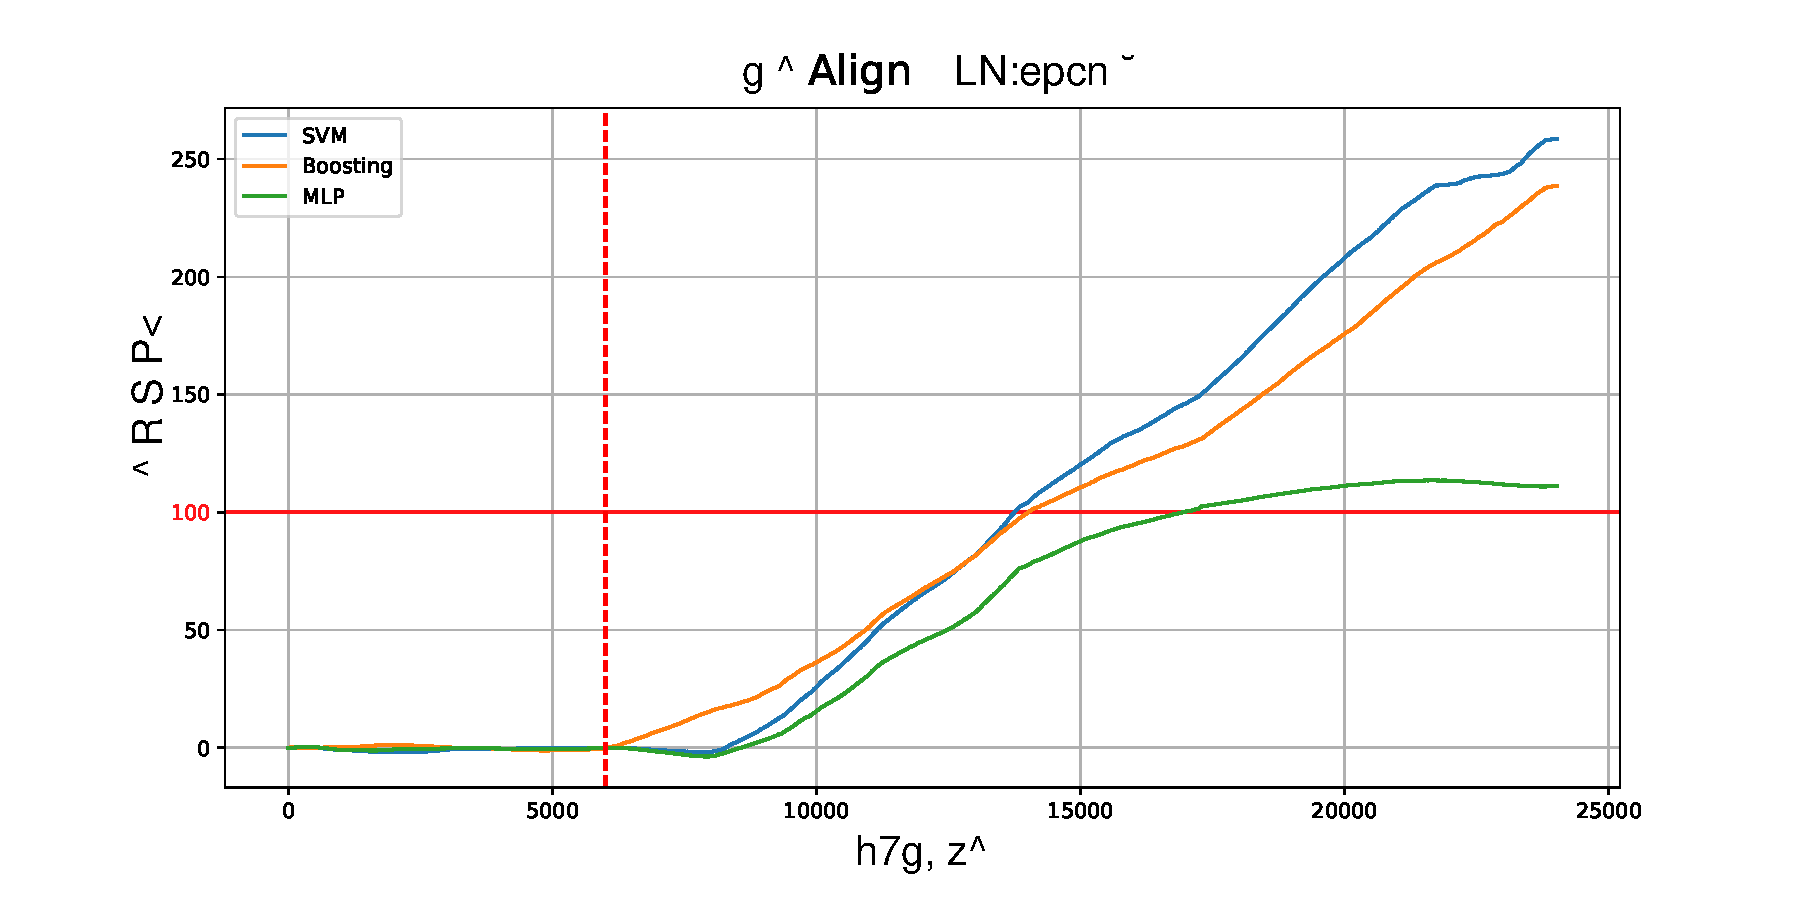
\includegraphics[width=1\linewidth]{Img/chapter9/Align data set-icml}}
\caption{{Align}行为数据集有序学习的鞅序列}
\label{fig:align-mar}
\end{figure*}
\begin{figure*}[htbp] % [tb]
\centerline{
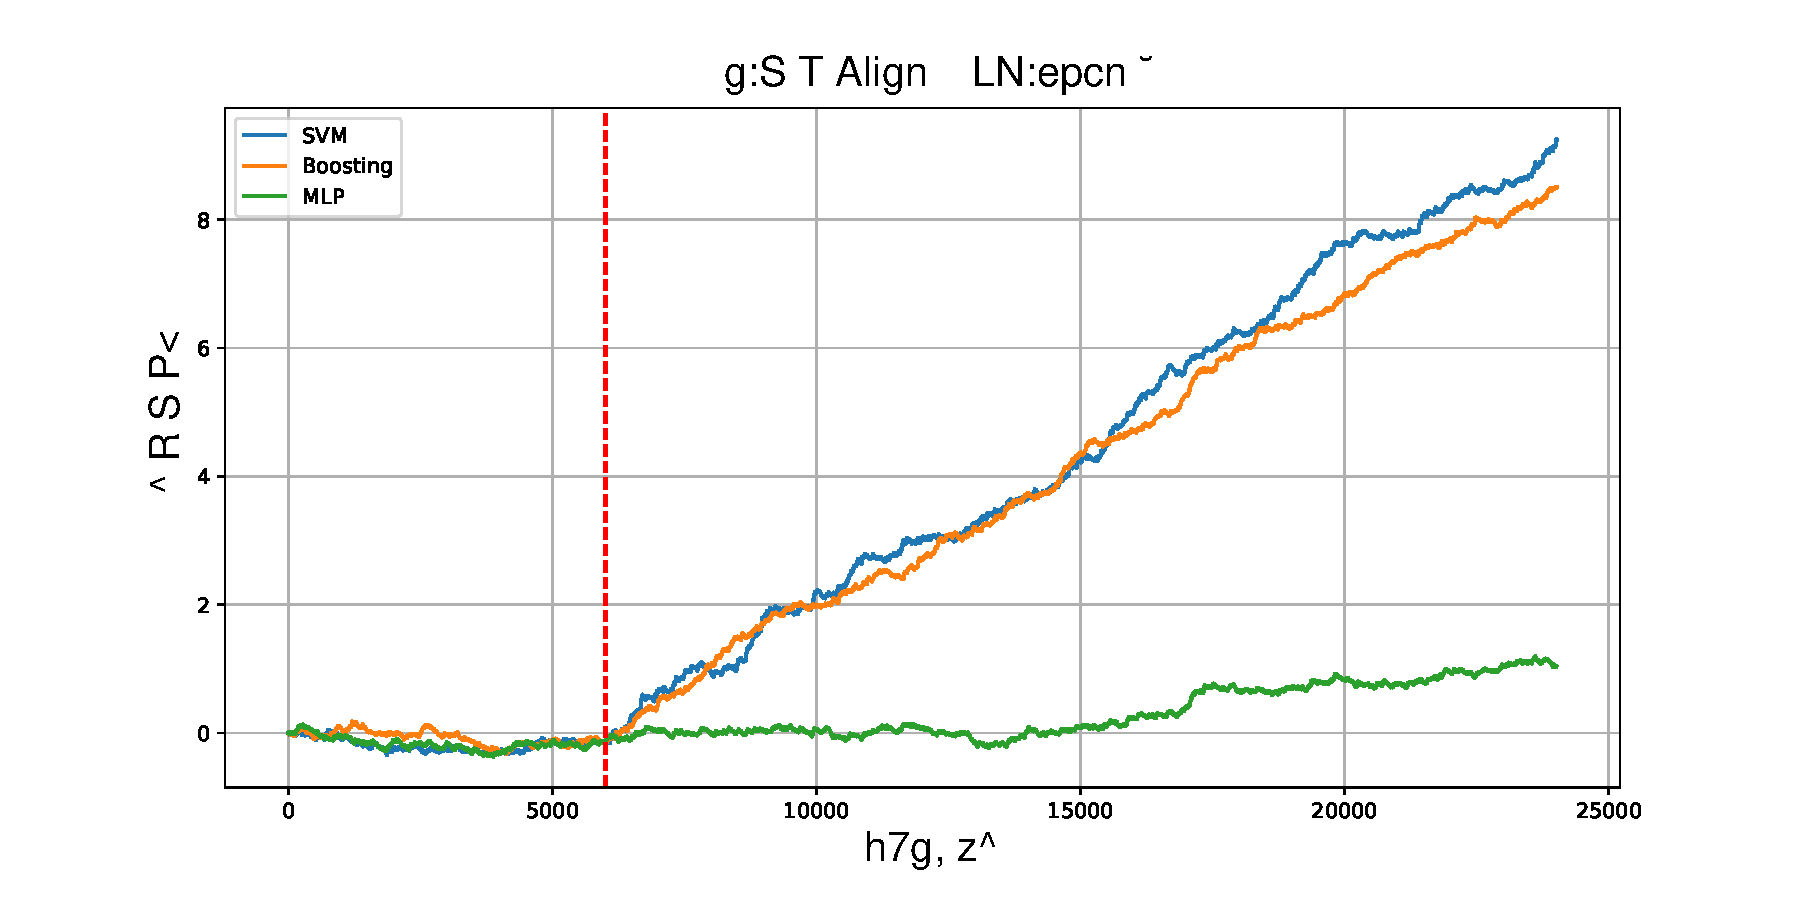
\includegraphics[width=1\linewidth]{Img/chapter9/Randomly shuffling Align data sett-icml}}
\caption{随机化{Align}行为数据集有序学习的鞅序列}
\label{fig:radom-align-mar}
\end{figure*}


其次, 对于Flock数据集, 图\ref{fig:flock-mar}展示三种机器学习算法计算得到的鞅序列。图\ref{fig:flock-mar}展示学习样本按照原始顺序进入模型后权力鞅序列的增长情形。 例如, 当采用全连接神经网络作为底层算法时, 权力鞅序列最终的取值大约是$210$, 权力鞅的最终值远远大于给定的阈值100。对于SVMs算法和Boosting 算法, 其最终的取值分别大约是$390$和$320$, 这两个取值也是远远大于给定的阈值100。 这说明对于Flock行为的无人机集群行为数据集, 如果按照数据本身时间顺序建模, 那么在训练集上得到的机器学习算法一定不能一直被当作“万能逼近”算子采用, 而应该在鞅序列大于阈值100处停下来。换言之, 对于Flock数据集而言, 如果采取保守策略, 对于SVMs算法和Boosting算法应该在大概第12000个测试样本左右(此时权力鞅的取值第一次达到阈值100左右)停止使用先前训练的机器学习算法; 对于神经网络算法大概应该在第14000个测试样本左右停止使用先前训练得到的算法。权力鞅的检测结果也证实表\ref{tab:online}中Flock数据集的预测表现, 即在保留数据本身顺序情形下构建的机器学习算法并没有提供极其优越的预测效果。

同样, 图\ref{fig:flock-mar}也表明对于不同的机器学习算法对Flock数据集的分布漂移展示出不同程度的鲁棒性。根据达到阈值100的样本量大小可知神经网络算法对于Flock数据集表现出更稳健的预测效果。但是由于鞅序列表达式(\ref{martingale-C})给出的结果是基于“依概率(in probability)”的结论, 所以神经网络在总体上的预测效果并没有比Boosting算法优越。然而对于分布漂移检测问题, 则可以肯定鞅序列方法提供高效的检测能力。

图\ref{fig:radom-flock-mar}展示三种机器学习算法在随机化处理后的Flock数据集上计算得到的鞅序列。图\ref{fig:radom-flock-mar}展示此情形下权力鞅序列的增长情形。图中结果表明随机处理Flock数据集后三种机器学习算法的权力鞅序列都没有大于阈值100, 因此可以判定在这种情形下三种机器学习算法都可以提供相当优越的预测结果。权力鞅的检测结果也证实表\ref{tab:offline}中Flock数据集的预测表现, 即随机化后的机器学习算法都提供优越的预测效果。

图\ref{fig:radom-flock-mar}更明显地表明即便利用随机采样的训练集构建机器学习模型可以得到相当满意的预测效果, 但是鞅序列仍然是保持了向上增长的趋势, 并且如果持续增加测试样本, 此序列也会缓慢超过给定阈值 (如果将阈值设定为更为严格的$C=20$, 那么SVMs算法下就已经指示出随机采样后的Flock数据也存在分布漂移)。这说明即便随机采样后数据满足独立同分布假设, 但是数据本身的分布漂移仍然是存在的。

\begin{figure*}[htbp] % [tb]
\centerline{
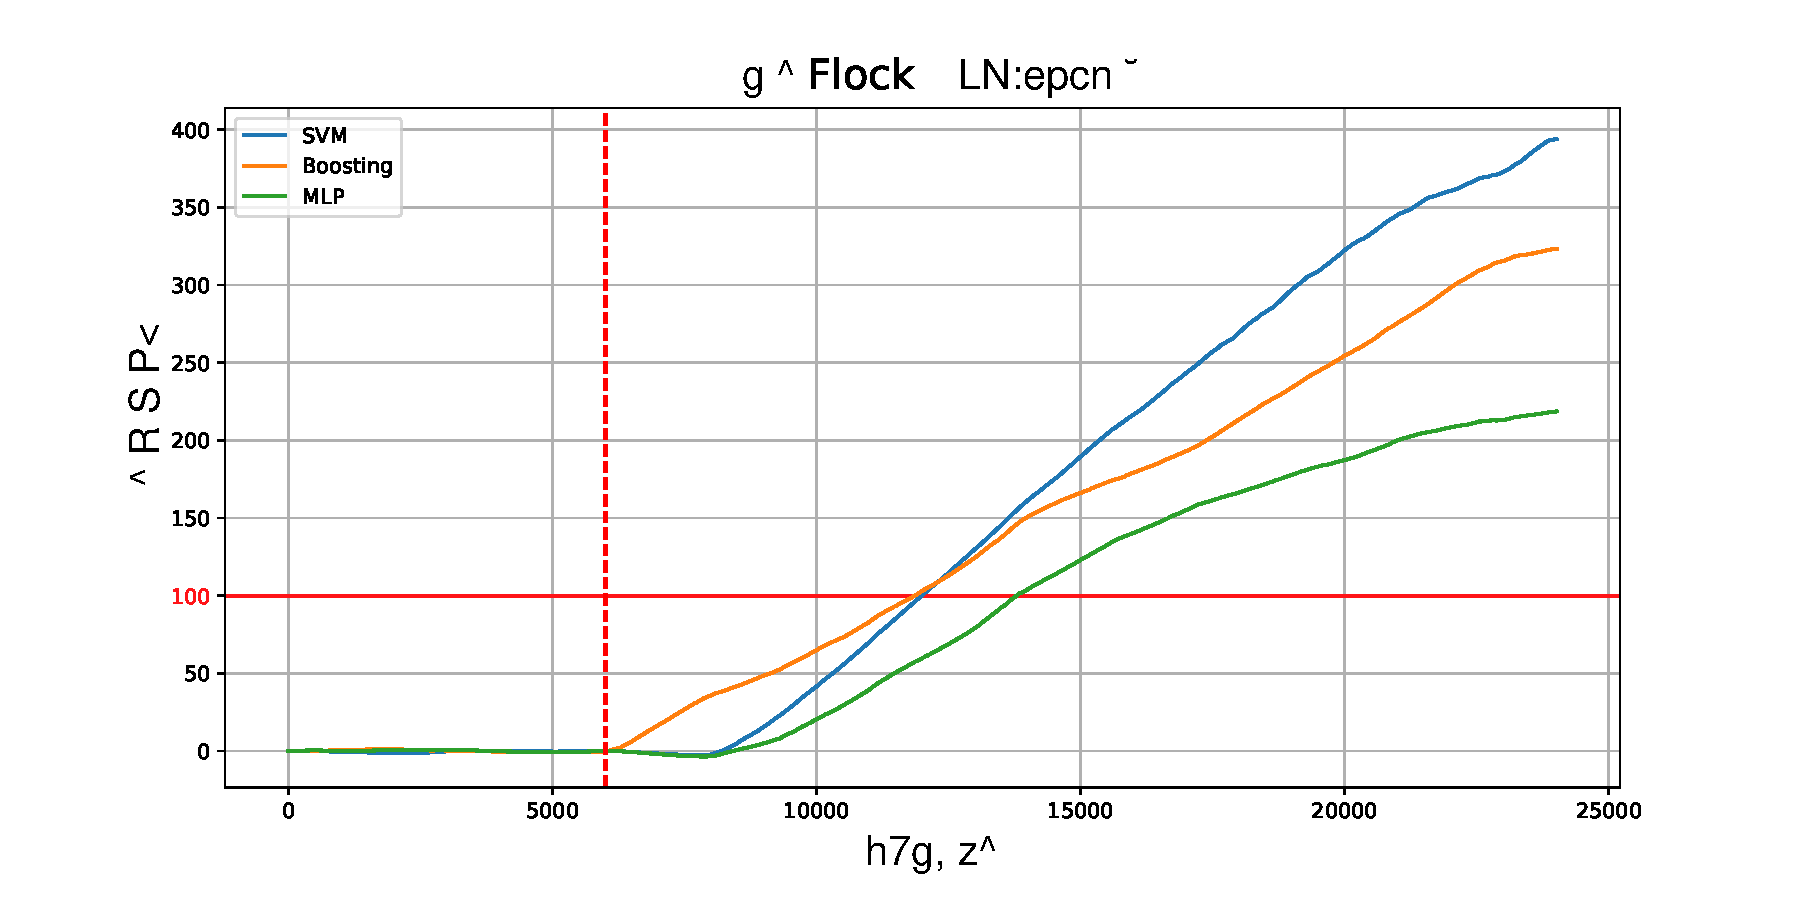
\includegraphics[width=1\linewidth]{Img/chapter9/Flock data set-icml}}
\caption{{Flock}行为数据集有序学习的鞅序列}
\label{fig:flock-mar}
\end{figure*}
\begin{figure*}[htbp] % [tb]
\centerline{
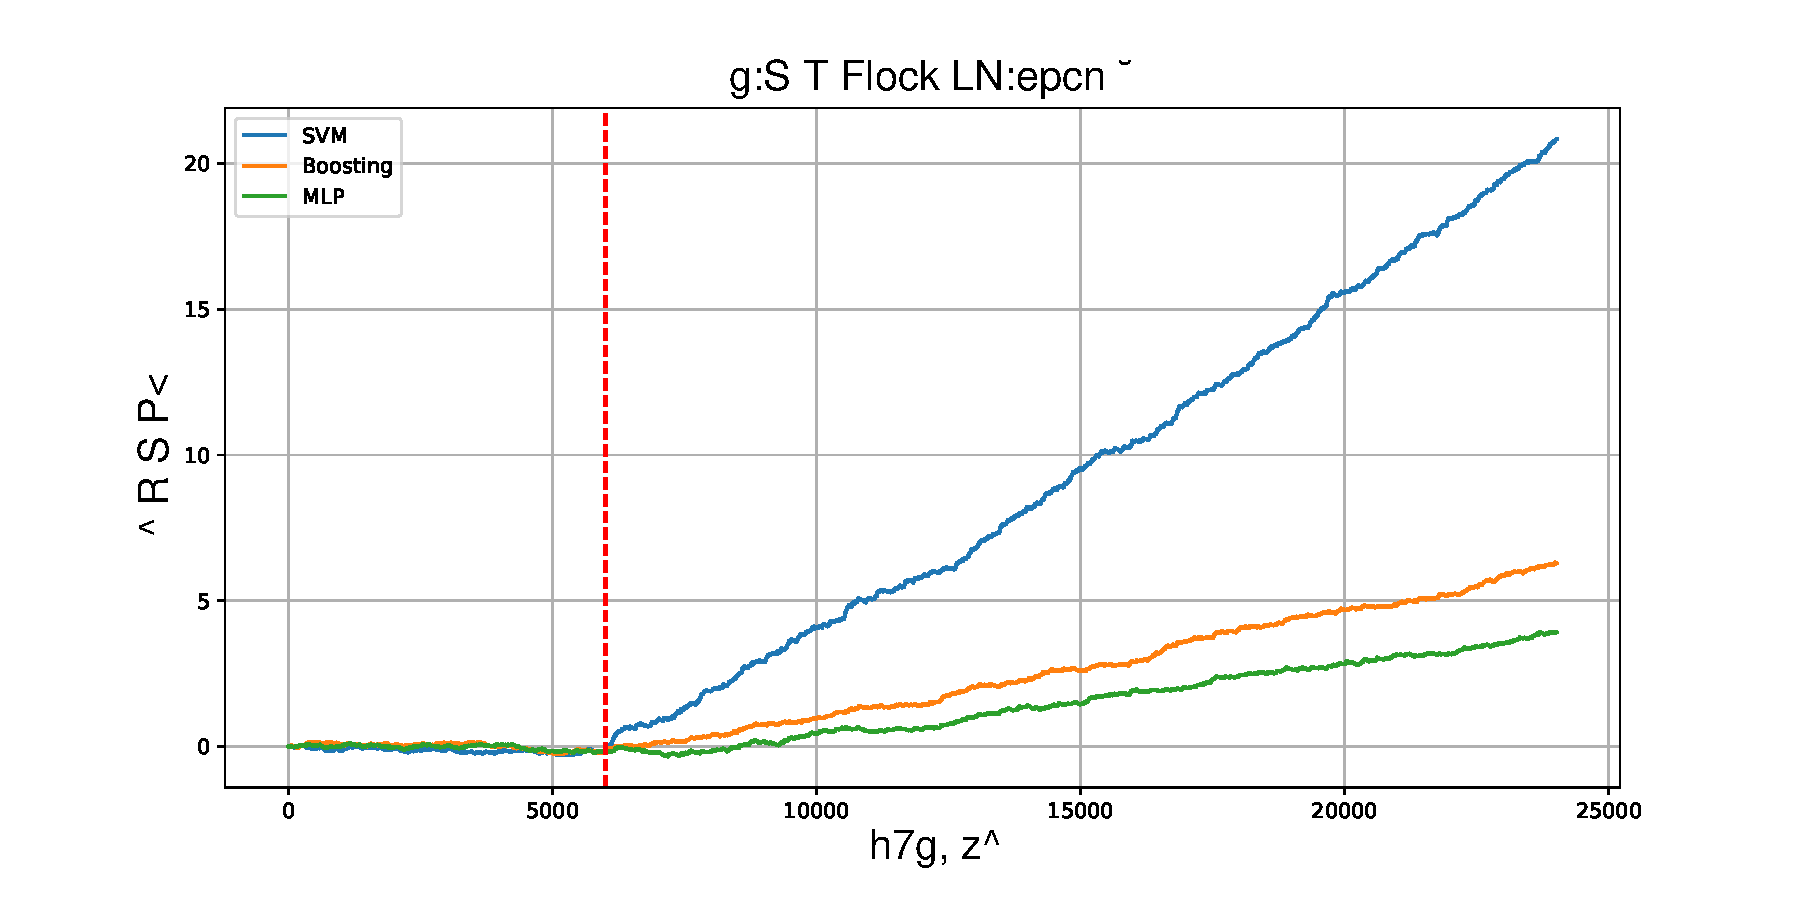
\includegraphics[width=1\linewidth]{Img/chapter9/Randomly shuffling Flock data sett-icml}}
\caption{随机化{Flock}行为数据集有序学习的鞅序列}
\label{fig:radom-flock-mar}
\end{figure*}


最后, 对于Group数据集, 图\ref{fig:group-mar}展示三种机器学习算法计算得到的鞅序列。当底层算法是Boosting时最先达到阈值100, 此时大约在第12000个样本达到阈值; 其次是SVMs算法, 其大约在第13000个样本时达到阈值100; 而当底层算法是神经网络算法时, 一直要持续到第15000个样本以后, 才达到阈值100。 这就是说, 对于Group数据集, 当底层算法是Boosting时, 大约在第12000个样本左右就可以拒绝零假设; 当底层算法是SVMs时, 大约在第13000个样本左右就可以拒绝零假设; 而底层算法是神经网络时, 一直到大约在第15000以后的样本才可以拒绝零假设。权力鞅的检测结果也证实表\ref{tab:online}中Group数据集的预测表现, 即在保留数据本身顺序情形下构建的机器学习算法并没有提供极其优越的预测效果。

与先前两种无人机集群行为数据相似, 图\ref{fig:radom-group-mar}展示三种机器学习算法在随机化处理后的Group数据集上计算得到的鞅序列。图\ref{fig:radom-group-mar}展示此情形下权力鞅序列的增长情形。图中结果表明随机处理Group数据集后三种机器学习算法的权力鞅序列都没有大于阈值100, 因此可以判定在这种情形下三种机器学习算法都可以提供相当优越的预测结果。权力鞅的检测结果也证实表\ref{tab:offline}中Group数据集的预测表现, 即随机化后的机器学习算法都提供优越的预测效果。

图\ref{fig:radom-group-mar}也表明即便利用随机采样Group数据集得到的训练集构建机器学习模型可以得到相当满意的预测效果, 但是鞅序列仍然是保持了向上增长的趋势, 并且如果持续增加测试样本, 此序列也会缓慢超过给定阈值(在随机化后的Group数据集中, SVMs最终取值达到17.5)。这说明即便随机采样后数据满足独立同分布假设, 但是数据本身的分布漂移仍然是存在的。

\begin{figure*}[htbp] % [tb]
\centerline{
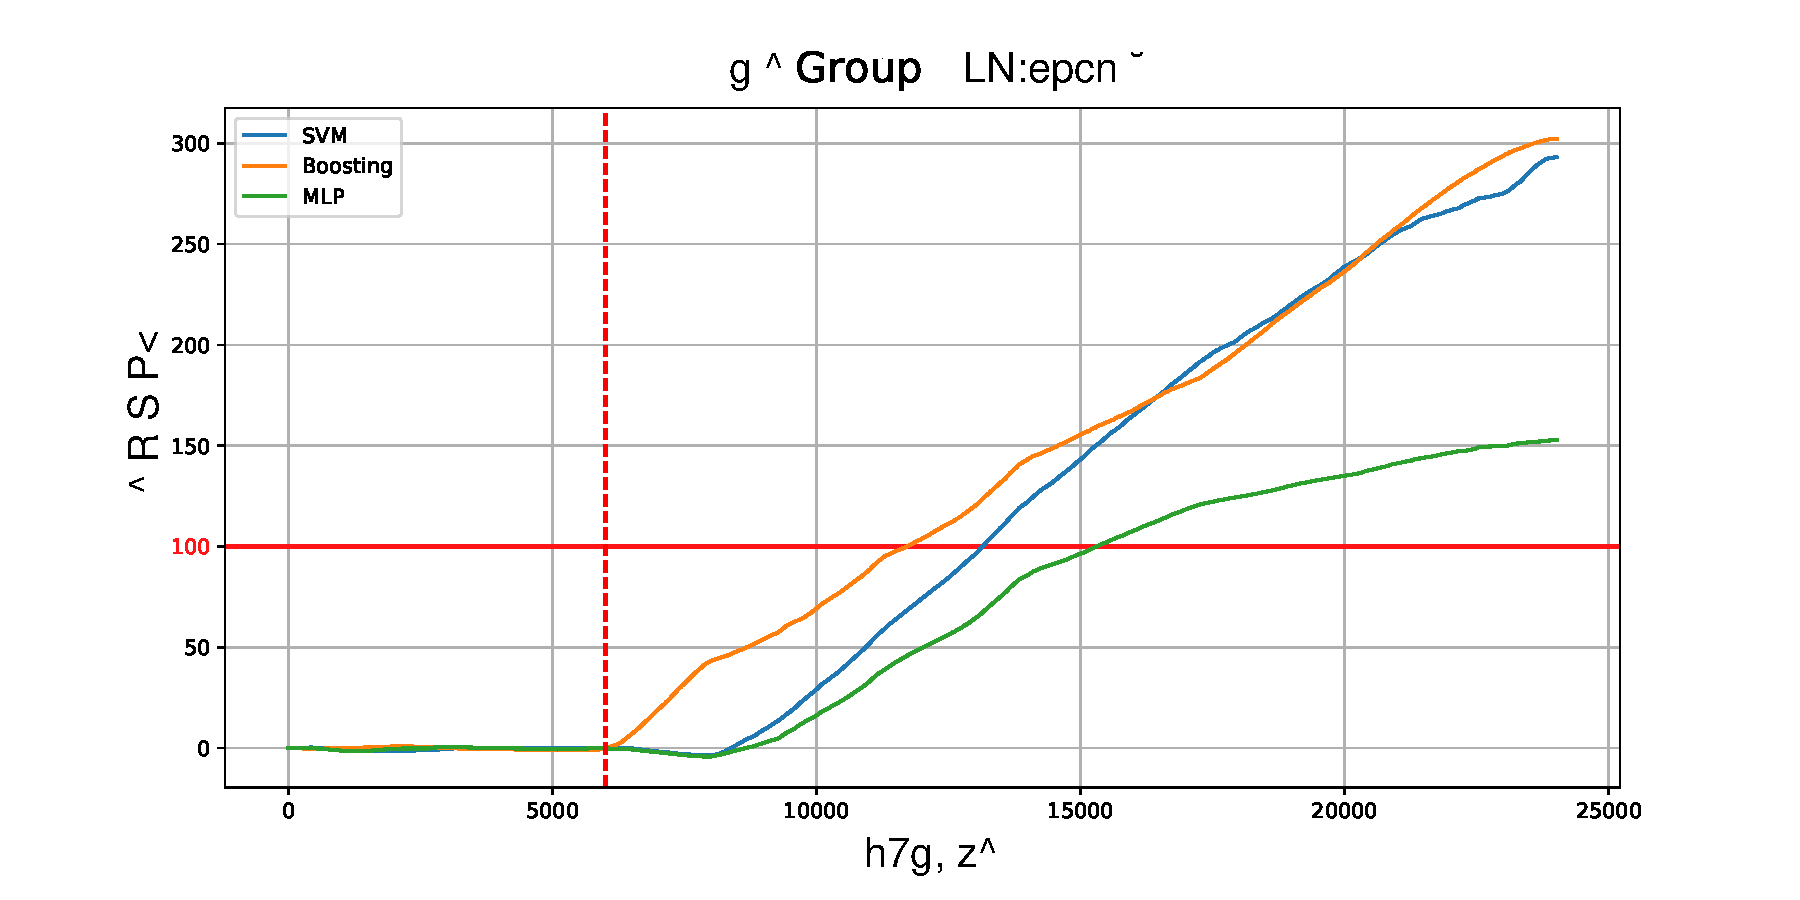
\includegraphics[width=1\linewidth]{Img/chapter9/Group data set-icml}}
\caption{{Group}行为数据集有序学习的鞅序列}
\label{fig:group-mar}
\end{figure*}
\begin{figure*}[htbp] % [tb]
\centerline{
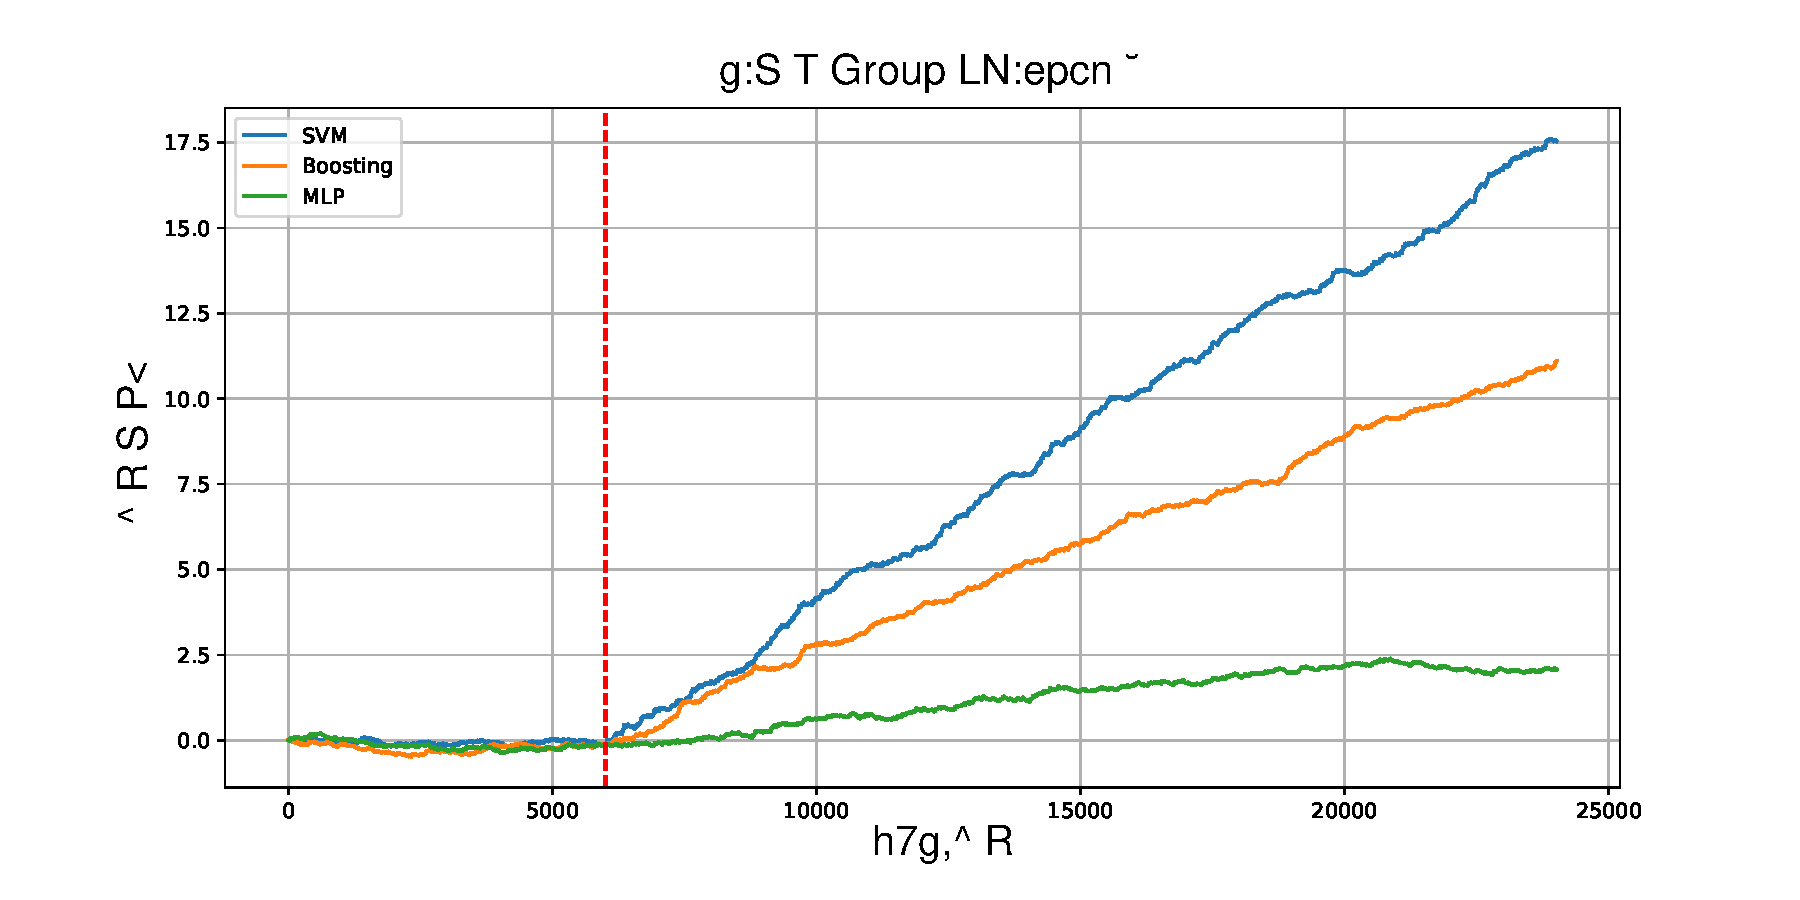
\includegraphics[width=1\linewidth]{Img/chapter9/Randomly shuffling Group data sett-icml}}
\caption{随机化{Group}行为数据集有序学习的鞅序列}
\label{fig:radom-group-mar}
\end{figure*}


\section{本章小结}
\label{sec:mar-discuss}
本章针对无人机集群行为数据的分布随着时间发生变化的特点, 结合鞅理论提出一种无分布假设的分布漂移检测方法。主要结论总结如下:
\begin{enumerate}
\item 在无人机集群数据按照本身时间顺序建模和随机采样建模两种情形下, 对比机器学习算法预测性能之间的差异。试验结果表明, 当按照数据本身顺序建模时, 机器学习算法预测错误数目远远大于随机采样情形下的预测数目;
\item 利用鞅方法检测无人机集群行为数据的分布漂移。试验结果表明, 样本数据按照本身顺序进入模型后, 鞅序列的值增长较快; 并且鞅序列取值远远大于给定阈值。根据鞅理论, 这种现象表明无人机集群行为数据发生分布漂移;
\item 对于随机采样后建模数据, 鞅序列取值虽然没有超过给定阈值, 但是鞅序列依然保持上涨的趋势。这说明对原始数据随机采样, 一方面可以获得更加高效的预测效果, 但是另一方面也说明即便是随机采样也无法消除数据本身分布漂移现象。
\end{enumerate}
\chapter{基于鞅保护分布方法的无人机集群行为分类研究}
\label{chapter:swarm-martingales}
\section{引言}
第\ref{chapter:swarm-distributions}章的结论表明实际工程数据自身的时间顺序是很重要的信息。在处理实际工程问题时, 不能轻易通过技术随机打乱实际工程应用中数据本身的时间信息。同时, 第\ref{chapter:swarm-distributions}章的结论也表明, 当按照数据本身时间顺序构建机器学习模型时, 模型的预测能力通常是有限度的。为提高实际工程问题中模型预测效果, 本章提出一种融合数据本身时间顺序的方法, 这种方法仍然是建立在底层机器学习算法之上的, 因此本章提出的算法依旧可以提升机器学习算法的预测效果。

第\ref{chapter:swarm-distributions}章的结论同时也表明随机化能够明显提高机器学习模型的预测效果。因此, 本章将第\ref{chapter:swarm-distributions}章研究的结论综合起来考虑: 本章中仍然处理实际工程应用中的有序学习问题, 虽然数据本身的时间顺序无法随机化, 但是本章可以为模型提供一种随机化方案, 即将模型中最外层具有固定形式的函数随机处理。本章仍然采用一致性预测思想实现这一目的。

\section{基于一致性预测的鞅保护分布方法理论研究}
\label{transductive}

本章围绕为考虑数据自身时间顺序的无人机集群数据展开高效的行为分类。 首先对于无人机集群行为分类问题, 将之归约为模式识别问题。正如第\ref{chap:edbed}章已经阐明的, 对于模式识别问题, 其基本假设是给定训练样本数据集由固定的、但未知的概率分布函数独立地生成。基于经验数据, 学习器在诸函数的集合——这些诸函数是由机器实现的——中挑选一个函数 $f(x, \alpha_{0})$, 此函数能够最小化错误分类数目。 目前的大多数机器学习方法都基于此问题假设, 形成一种离线学习框架。 使用一批学习样本得到某规则函数, 进而将规则函数应用于测试样本。 这样的工作在集群学习领域已经有众多的研究文献。 例如, \citet{Brown2014} 基于受限带宽情形下利用机器学习算法识别集群行为分类; \citet{Berger2016}提出一种压缩子空间的方法实现集群行为分类方法; \citet{Thomas2021}则将集群整体看做动态系统来揭示集群行为所产生的影响。

然而, 由于本章考虑按照实际工程中数据本身的时间顺序预测无人机集群行为, 因此需要针对有序学习展开讨论。保留实际数据自身时间顺序的有序学习属于超越推理范式\citep{vapnik1995,vapnik1998}。 超越推理是由Vapnik提出的一种新的学习范式, 这种学习范式考虑为保留时间顺序的真实数据提供预测估计。在技术层面而言, 与超越推理对应的传统统计学基于归纳推理范式。归纳推理范式需要两步完成推理, 首先需要估计一般函数参数, 然后再将新观测数据输入估计函数得到预测值\citep{Fisher1956}。 与此相反, 超越推理利用经验数据直接得到对应的函数的值, 这种推理范式由于和实际工程问题高度匹配, 近些年受到越来愈多研究者的关注\citep{Becker2014,Luc2014}。也就是说, 根据超越推理范式, 观测到第一个对象$x_{1}$后开始预测对应的标签$y_{1}$; 然后观测到第二个对象$x_{2}$后开始预测其标签$y_{2}$, 以此类推。因此在这种推理范式下不允许研究者提前随机化数据。

由于在超越推理范式下无法随机化数据, 因此数据本身无法满足独立同分布的假设条件, 所以在处理实际问题时总会遇到分布漂移的问题。同时经过第\ref{chapter:swarm-distributions}章的研究已经表明, 实际工程数据自身的时间顺序是很重要的信息。为此, 本章提出一种将数据本身时间顺序纳入底层机器学习算法来增强底层机器学习算法的泛化推广能力。

\subsection{鞅保护分布方法研究现状}
考虑数据本身时间顺序的研究主要由Vovk提出。可以采用各种不同的分布漂移解决方案提升机器学习的学习能力。例如, \citet{Vovk2021retrain}提出通过鞅序列检测理论给出的分布漂移位点指示, 当鞅序列取值大于给定阈值时, 可以对学习模型进行二次训练以提升预测性能。但是则从另一个角度出发, 通过将考虑数据本身时间顺序的鞅序列融合至底层算法, 这样就无需二次训练而直接提升底层算法的预测效果。\citet{Vovk2021protectedregression}首次提出基于一致性预测的鞅保护分类方法, 并首先将之应用于处理回归问题。同样的\citet{Vovk2021protectedclassification}后来将提出的基于一致性预测方法的鞅保护分布方法应用于分类问题。 注意到这项工作后, 便将之引入无人机集群行为分类研究领域, 以期通过鞅保护分布的分类方法来提升有序学习时机器对复杂无人机集群行为的辨识能力。 

鞅保护分布算法的优点在于其可以作用于机器学习算法顶层, 通过对机器学习算法的输出——称之为暴力得分函数——进行鞅保护分布方法校正以获得更好的预测能力。因为受到底层机器学习算法的支撑, 这种方法可以克服“维数灾难”问题, 能够处理任意的超高维问题。图\ref{fig:align-example}展示鞅保护SVMs算法和鞅保护神经网络算法与无保护措施SVMs算法和无保护措施神经网络算法在预测问题上的对比, 模型的预测效果采用ROC曲线作为评价指标。图\ref{svm-1} 展示的是鞅保护SVMs算法的提升效果, 从图中可以看到未经鞅保护分布算法的SVMs算法预测的ROC曲线面积——即AUC值——为0.654, 经过鞅保护分布算法提升后其预测AUC值提升为0.734; 图\ref{nn-1} 展示的是鞅保护神经网络算法的提升效果, 从图中可以看到未经鞅保护分布算法的神经网络算法预测的AUC值为0.517, 经过鞅保护分布算法提升后其预测AUC值提升为0.724。图\ref{fig:align-example}给出的例子说明鞅保护分布算法能够明显提升底层机器学习算法的预测能力。

本章首先介绍鞅保护分布算法的理论, 然后将提出的鞅保护分布算法应用于处理无人机集群行为分类问题, 构建无人机集群鞅保护分布算法, 形成一套端到端的并且可建立在机器学习算法顶层的鞅保护分布框架。 因为引入鞅保护分布后数据本身的时间顺序得到考量, 因此对于实际工程中遇到的真实数据分析任务能够提供相当可观的提升效果。

%\begin{figure*} % [tb]
%\begin{center}
%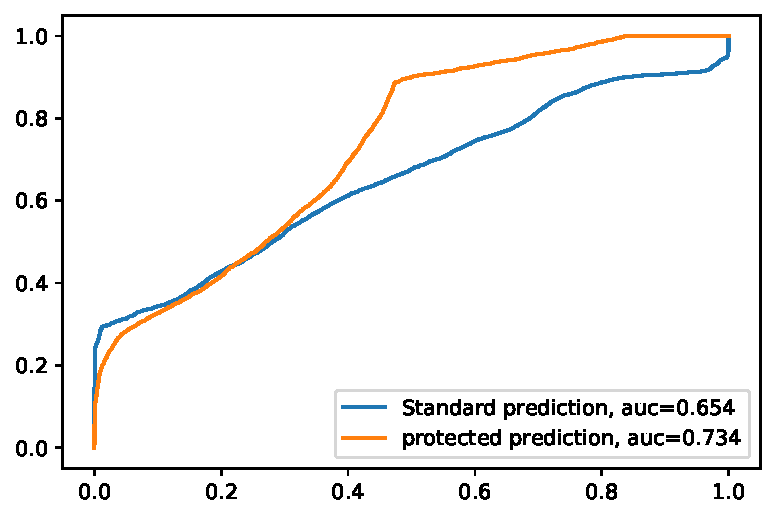
\includegraphics[scale=.5]{Img/chapter11/align-SVC}
%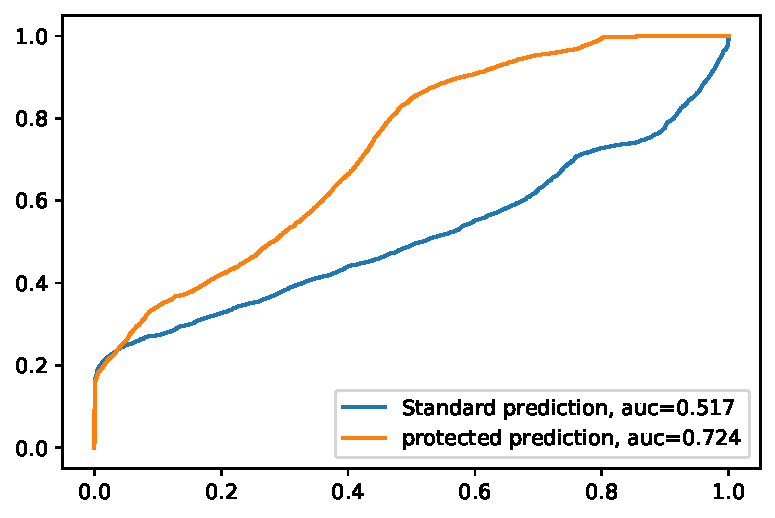
\includegraphics[scale=.5]{Img/chapter11/align-MLPClassifier}
%\end{center}
%\caption{鞅保护SVMs和鞅保护神经网络算法分类结果示例}
%\label{fig:align-example}
%\end{figure*}
%

\begin{figure}
     \centering
     \begin{subfigure}[b]{.45\textwidth}
         \centering
         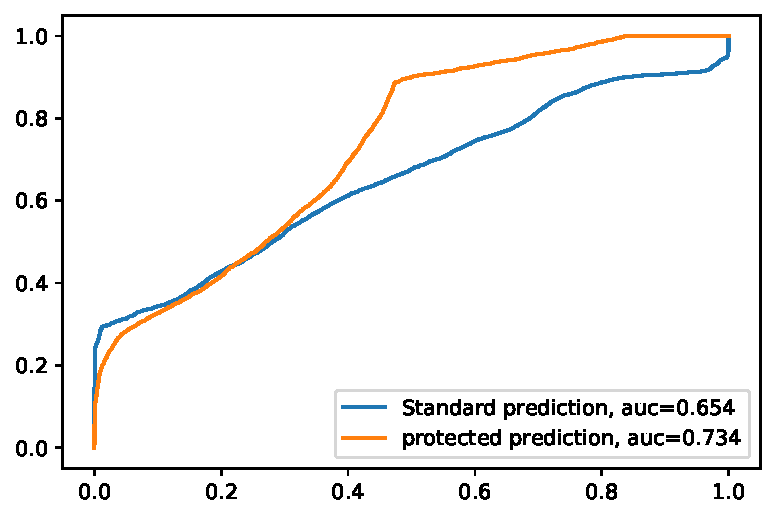
\includegraphics[width=1\textwidth]{Img/chapter11/align-SVC}   
         \caption{SVMs鞅保护算法分类结果}
         \label{svm-1}
     \end{subfigure}
     \hfill
     \begin{subfigure}[b]{.45\textwidth}
         \centering
         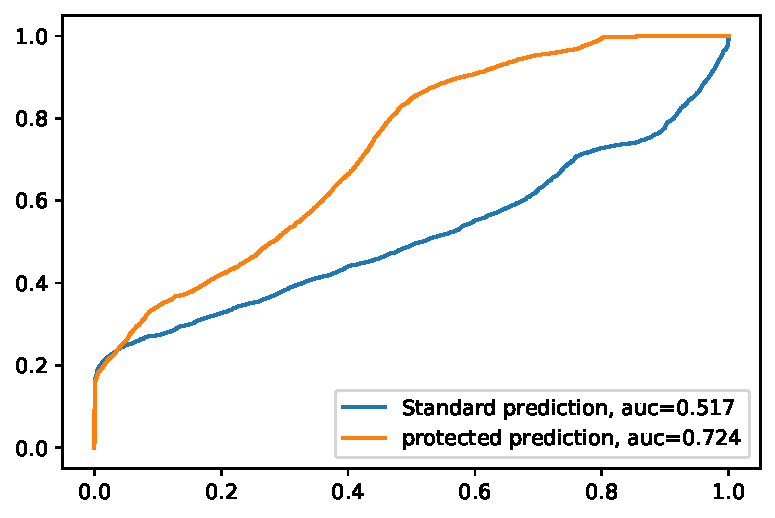
\includegraphics[width=1\textwidth]{Img/chapter11/align-MLPClassifier}
         \caption{神经网络鞅保护算法分类结果}
         \label{nn-1}
     \end{subfigure}
\caption{鞅保护SVMs和鞅保护神经网络算法分类结果示例}
\label{fig:align-example}
\end{figure}

\subsection{鞅保护分布方法理论研究}
本节介绍鞅保护分布方法的理论。根据第二章研究的VC理论, 学习机器推广泛化能力的控制是由两个因素决定的, 即不仅仅需要控制训练误差, 而且需要控制容量$h$。 通过鞅保护分布方法可以提升学习器的推广泛化能力, 此方法通过随机化模型最外层函数的具体形式, 将单一函数转变为“模糊函数带”来实现目标, 这相当于增加函数的丰富程度。


为实现在VC理论指导下鞅保护分布算法泛化推广能力的控制, 根据第\ref{chapter:swarm-distributions}章介绍的一致性鞅理论, 引进新的博弈函数。 博弈函数由两个抽象参数控制, 分别是跳跃参数 (Jumper) $J$ 和函数参数 $\theta$。 给定新的校正函数
\begin{align}
f_{\theta}: [0,1] \rightarrow [0,1], \theta \in \Theta.
\end{align}
直观而言, 引进这种新的校正函数是希望通过此校正函数能够将原初机器学习算法的得分函数 $p_{n}$ 改进为校正后函数$f_{\theta}(p_{n})$, 并且希望校正后函数$f_{\theta}$能够提升底层学习算法的泛化推广能力。 

但是在鞅保护分布算法中, 提前并不知道到底哪个校正函数$f_{\theta}$是最佳的, 并且希望函数的参数$\theta$取值随时间变化。 因此, 基于 \citet{Vovk2021protectedclassification} 提出的“专家经验追踪”法 (“tracking the best expert”)来实现校正函数的获取。 具体而言, 使用Cox函数作为校正函数, 即
\begin{align}
f_{\alpha,\beta}(p):=\frac{p^{\beta}\exp(\alpha)}{p^{\beta}\exp(\alpha) + (1-p)^{\beta}},
\end{align}
其中, 这里函数参数 $(\alpha,\beta) = \theta \in \mathbb{R}^2$, 其中 $\alpha \in \{0,1,-1\}$, $\beta \in \{1,0.5,2\}$。 

在此校正函数定义下列初等鞅检测函数(elementary test martingale),
\begin{align}
\prod_{n=1}^{n}\frac{B_{f_{\theta_{i}}(p_{i})}(\{y_{i}\})}{B_{p_{i}}(\{y_{i}\})},n=0,1,\ldots
\end{align}
其中, 这里 $B_{p}, p \in [0,1]$是服从参数为$p$的$\{0,1\}$上的Bernoulli分布随机变量: $B_{p}(\{1\}) = p$。 设定算法“专家经验追踪”法中另一个参数跳跃速度$J \in [0,1]$, 则可以得到基于一致性预测的跳跃鞅序列, 此算法计算了每个机器学习算法输出$p_{i}$对应的跳跃鞅$S_{i}$。 算法\ref{alg:betting}给出基于一致性预测的跳跃鞅(Jump-Martingales)序列算法整个框架。

\begin{algorithm}[!htbp]
    \small
    \caption{基于一致性预测跳跃鞅序列算法(Jump-Martingales)}
    \label{alg:betting}
    \hspace*{\algorithmicindent} \textbf{输入:} {($p_{1}, p_{2}, \ldots$).}\\
    \hspace*{\algorithmicindent} \textbf{输出:} {($S_{1}, S_{2}, \ldots$).}
    \begin{algorithmic}[1]
        \Procedure{Jump-Martingales}{}
        \State 设定初始参数$C_{\theta} := 1/|\Theta|$, $\theta \in \Theta$,
    		\State $C := 1$,
        \For{$n=1,2, \ldots$}
        \For{$\theta \in \Theta$}
        \State $C_{\theta} := (1-J)C_{\theta} + (J/|\Theta|)C$,
        \EndFor
        \For{$\theta \in \Theta$}
        \State $C_{\theta} := C_{\theta}\frac{B_{f_{\theta}(p_{n})}(\{y_{n}\})}{B_{p_{n}}(\{y_{n}\})}$,
        \EndFor
        \State $S_{n} := C := \sum_{\theta \in \Theta}^{} C_{\theta}$.
        \EndFor
        \EndProcedure
    \end{algorithmic}
\end{algorithm}

\section{基于一致性预测的鞅保护分布方案设计}
现在针对由函数参数$(\theta_{1},\theta_{2},\ldots) \in [0,1]^{\infty}$上定义的概率测度$\mu$, 通过“去随机化”处理以上随机测试鞅。 定义下列表达式
\begin{align}
S_{n} := \int\prod_{i=1}^{n}\frac{B_{f_{\theta_{i}}(p_{i})}(\{y_{i}\})}{B_{p_{i}}(\{y_{i}\})}\mu(d\theta),
\end{align}
将之称为 “确定的测试鞅”(deterministic test martingale)。

给定机器学习算法 $A$, 定义此机器学习算法的gale指标\citep{glenn-vovk2019}, 即此函数将任意有限序列映射为下列乘积表达式$B_{p_{1}}(y_{1})\ldots B_{p_{n}}(y_{n})$, 其中, $n$是观测样本的个数, $y_{1},\ldots,y_{n}$ 是对应样本的标签, $p_{1},\ldots,p_{n}$ 是机器学习算法的预测输出。

在上述跳跃鞅序列算法中, 假设跳跃速率 (Jumping Rate) $J$ 在算法\ref{alg:betting} 中是提前已知的。现在对此做出修正, 提出复合跳跃鞅 (Composite Jumper martingales)。 这种方法依赖于两个参数, 初始状态 $\pi \in (0,1)$ 和 有限的非零跳跃比率集合 $J \in \{0.01, 0.001, 0.0001\}$。 据此可以定义下列加权平均后的跳跃鞅
\begin{align}
S_{n} := \pi + \frac{1-\pi}{|\mathbf{J}|}\sum_{J \in \mathbf{J}}S_{n}^{J},
\end{align}
其中, 这里 $S^{J}$ 是简单跳跃鞅 (Simple Jumper martingale)。

综上所述, 可以给出完整的鞅保护分布算法。此算法为机器学习算法输出$p_{i}$在鞅保护分布下给出新的校正函数$p_{i}^{\prime}$。 对于每个跳跃速率 $J \in \mathbf{J}$, 每个函数参数 $\theta = (\theta_{1}, \theta_{2},\ldots)$, 计算受保护的预测值
\begin{align}
p_{n}^{\prime} := f_{\theta_{n}}(p_{n}),  n=1,2,\ldots.
\end{align}

因为需要将底层机器学习算法和受保护的预测值进行统一尺度下的比较, 所以制定下列统一损失函数作为对比尺度, 即
\begin{equation}
  \lambda(y,p) :=
    \begin{cases}
      -\log{p} & \text{if $y=1$}\\
      -\log{(1-p)} & \text{if $y=0$,}
    \end{cases}       
\end{equation}
其中这里 $y \in \{0,1\}$ 是真实标签, $p \in [0,1]$ 是其对应的预测得分值。

算法 \ref{alg:protect} 完整给出基于一致性预测鞅保护分布(Distributions-Protected)校正算法。 在集群行为分类问题研究中, 选择多种机器学习算法作为底层算法。 例如, 可以选择SVMs, 神经网络, Boosting和 Na\"{i}ve Bayes 等机器学习算法输出得分函数 $(p_1, p_2, \ldots)$, 然后基于算法\ref{alg:protect}计算经过鞅保护分布后的得分函数 $(p_1^{\prime}, p_2^{\prime}, \ldots)$。

\begin{algorithm}[!htbp]
    \small
    \caption{基于一致性预测鞅保护分布校正算法(Distributions-Protected)}
    \label{alg:protect}
    \hspace*{\algorithmicindent} \textbf{输入:} {($p_{1}, p_{2}, \ldots$).}\\
    \hspace*{\algorithmicindent} \textbf{输出:} {($p_{1}^{\prime}, p_{2}^{\prime}, \ldots$).}    
    \begin{algorithmic}[1]
        \Procedure{Distributions-Protected}{}
        \State 设定初始参数$C_{\theta} := 1$, $\theta \in \Theta$,
        \For{$n=1, 2, \ldots$}
        \State $C := \sum_{\theta \in \Theta}^{}C_{\theta}$,
        \For{$\theta \in \Theta$}
        \State $C_{\theta} := C_{\theta}/C$,
        \EndFor
        \For{$\theta \in \Theta$}
        \State $C_{\theta} := (1 - J)C_{\theta} + J/|E|$,
        \EndFor
        \State $p_{n}^{\prime} = \sum_{\theta \in \Theta}^{}f_{\theta}(p_{n})C_{\theta}$,
        \EndFor
        \For{$\theta \in \Theta$}
        \State $C_{\theta} := C_{\theta} B_{f_{\theta}(p_{n})}(\{y_{n}\})$.
        \EndFor
        \EndProcedure
    \end{algorithmic}
\end{algorithm}


\section{基于鞅保护分布方法的无人机集群行为分类}
\label{experimental}
本节介绍使用鞅保护分布方法解决无人机集群行为识别问题。选择SVMs, 神经网络, 决策树, 随机森林, 朴素贝叶斯 (Na\"{i}ve Bayes) 和 逻辑回归 (Logistic Regression) 分别作为底层算法并将这些算法与采用鞅保护分布算法增强后的预测效果作对比, 选择ROC曲线和对应的AUC值作为模型之间的对比评价指标。

仍然采用公开的真实集群行为数据集, 其数据来自澳大利亚新南威尔士大学的有序调查。 包含三种集群行为数据集: Align, Flock和 Group三种行为。将数据集合按照原始顺序划分为6004个训练样本, 剩余的18011个样本作为测试样本。如前所述, 每个样本的属性描述在前章节的表\ref{tab:datainfo}中列出, 本章所用到的数据集合特征描述在前章节表\ref{tab:train_test1}中给出, 仍然仅仅选择位置坐标作为输入变量。 使用开源机器学习平台 scikit-learn 中StandardScalar方法标准化数据, 各个底层算法模型均采用默认参数。 最后, 因为使用底层机器学习算法时总是需要获得 [0, 1] 之间基础预测值, 而如果对基础预测值不做截断处理, 会使得利用鞅保护分布算法中的损失函数失效 (因为损失函数中需要计算对数), 因此按照下列表达式对底层算法的输出做统一截断处理, 即使用下列表达式中的 $p^{*}$ 代替底层学习算法的输出 $p$,
\begin{equation}
  p^{*} =
    \begin{cases}
      \epsilon & \text{if $p \leq \epsilon$}\\
      p & \text{if $p \in (\epsilon, 1-\epsilon)$,}\\
      1-\epsilon & \text{if $p \geq 1-\epsilon$}
    \end{cases}       
\end{equation}
其中, 这里的阈值设定为$\epsilon := 0.01$。 使用训练数据得到底层算法, 一旦得到底层算法后不再会使用训练数据。 因此, 本节中的图示都是从测试数据开始的。

首先检验鞅保护分布算法对于神经网络类算法的提升效果。 鞅保护分布算法中跳跃速率设定为 $\mathbf{J} := \{0.01,0.001,0.0001\}$, 函数参数 $\theta = (\alpha, \beta)$ 的取值范围设定为$\alpha \in \{-1,0,1\}$ 和 $\beta \in \{0.5, 1, 2\}$。 图 \ref{mlp-jump} 展示的复合跳跃鞅在测试集上的取值, 可以看到明显数据分布是发生变化的(这部分内容在第\ref{chapter:swarm-distributions}章中采用鞅方法的分布漂移检测中已经讨论过)。 本章节的目标就是要利用这种变化来校正底层算法。

将鞅保护分布算法应用在底层神经网络算法之上, 可以得到利用校正后 $p^{\prime}$ 实现的分类任务所得结果。 图 \ref{mlp-jump-martingale-align} 对比标准底层机器学习算法和经过鞅保护分布增强后预测算法最终的ROC得分。 从图中可以看出, 经过鞅保护分布措施后原先的神经网络算法其分类AUC值由0.517提升至0.724, 很明显借助鞅保护分布方法为底层神经网络提供的提升是显著的。

%\begin{figure} % [tb]
%\begin{center}
%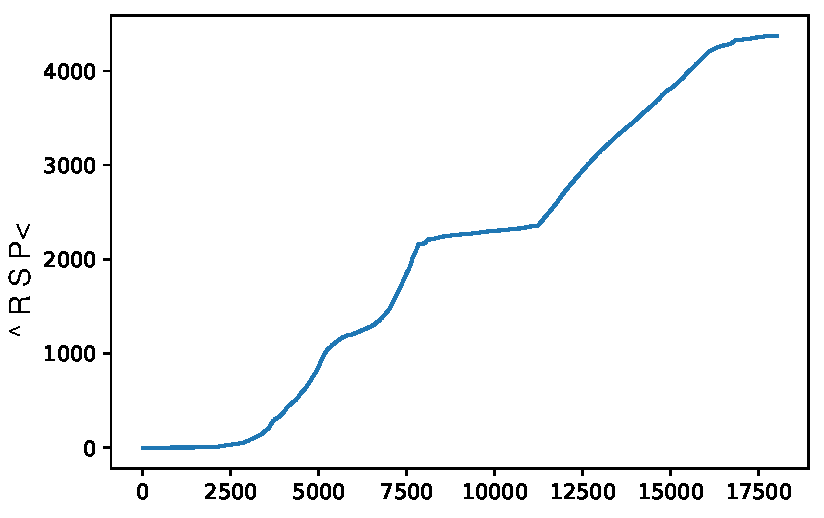
\includegraphics[width=0.4\textwidth]{Img/chapter11/align-martingale-MLPClassifier}
%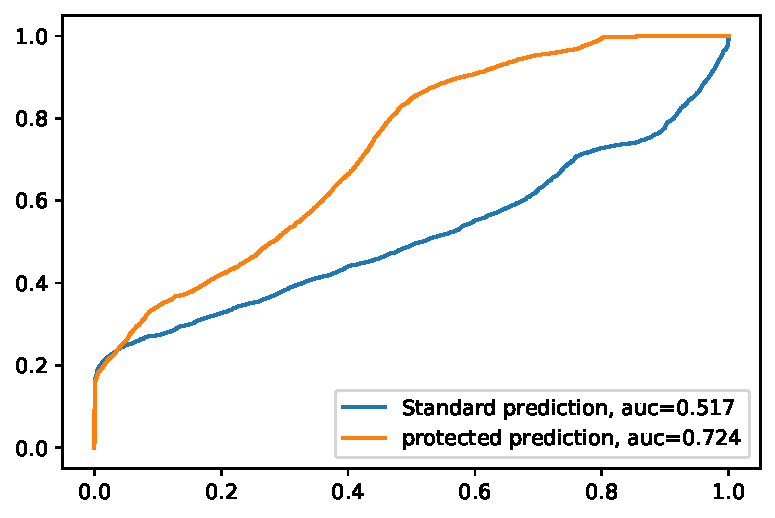
\includegraphics[width=0.4\textwidth]{Img/chapter11/align-MLPClassifier}
%\end{center}
%\caption{Align数据集的复合跳跃鞅以及鞅保护分布算法结果}
%\label{fig:align}
%\end{figure}

\begin{figure}
     \centering
     \begin{subfigure}[b]{.45\textwidth}
         \centering
         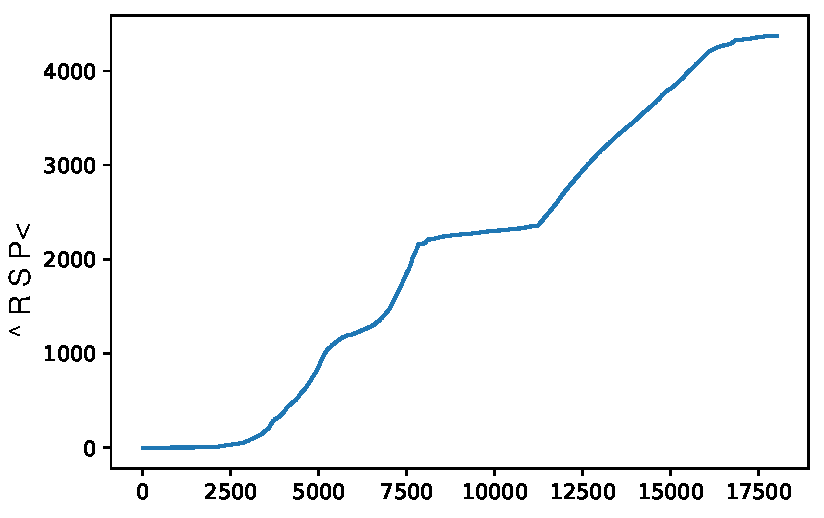
\includegraphics[width=1\textwidth]{Img/chapter11/align-martingale-MLPClassifier}   
         \caption{Align数据集的复合跳跃鞅}
         \label{mlp-jump}
     \end{subfigure}
     \hfill
     \begin{subfigure}[b]{.45\textwidth}
         \centering
         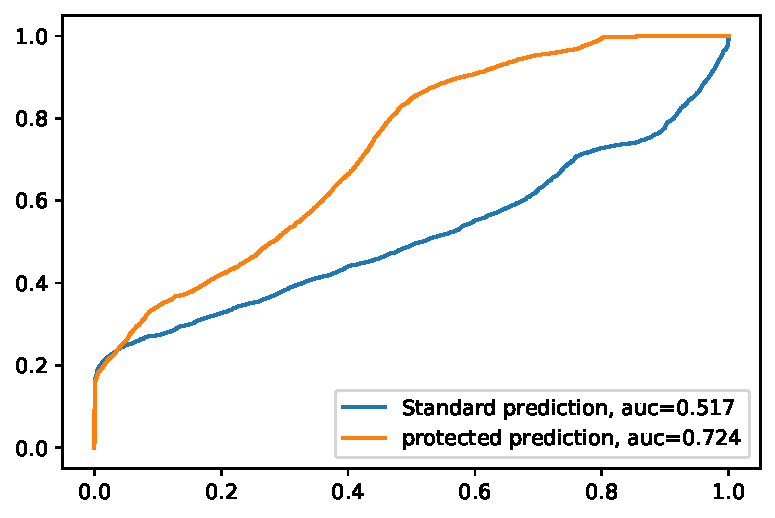
\includegraphics[width=1\textwidth]{Img/chapter11/align-MLPClassifier}
         \caption{Align数据集鞅保护分布算法结果}
         \label{mlp-jump-martingale-align}
     \end{subfigure}
\caption{Align数据集的复合跳跃鞅以及鞅保护分布算法结果}
\label{fig:align}
\end{figure}

对于Flock 数据集, 图\ref{mlp-jump-flock} 给出的是复合鞅序列, 类似的可以看到Flock数据集也发生分布漂移。 利用这种分布变化, 基于鞅保护分布算法校正底层神经网络算法。 图\ref{mlp-jump-martingale-flock} 给出校正后的ROC得分比较。 很明显, 通过鞅保护分布算法针对Flock数据集的底层神经网络的AUC值从0.63提升至0.715。 

%\begin{figure} % [tb]
%\begin{center}
%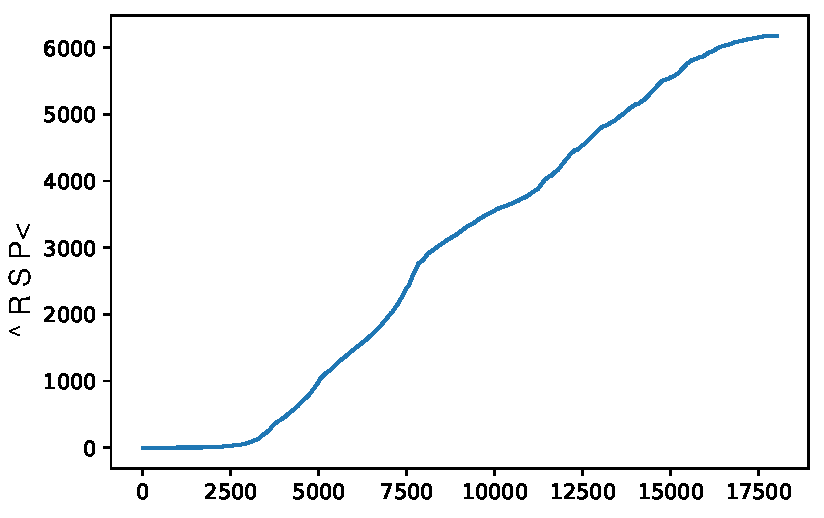
\includegraphics[width=0.4\textwidth]{Img/chapter11/flock-martingale-MLPClassifier}
%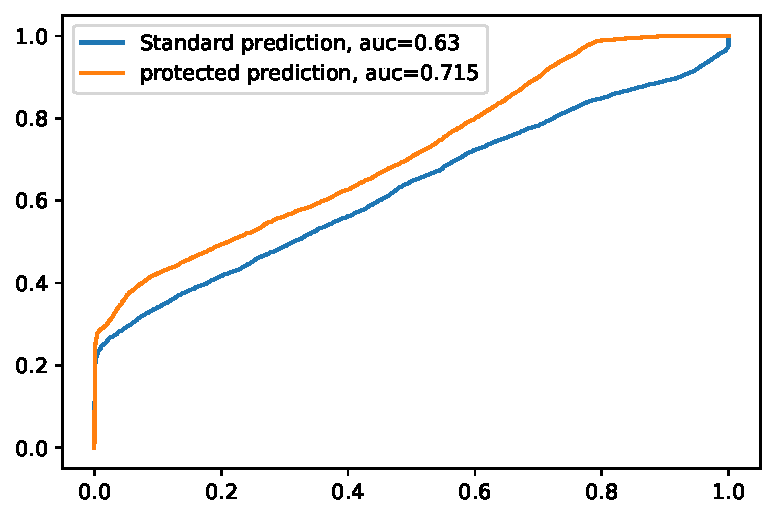
\includegraphics[width=0.4\textwidth]{Img/chapter11/flock-MLPClassifier}
%\end{center}
%\caption{Flock数据集的复合跳跃鞅以及鞅保护分布算法结果}
%\label{fig:flock}
%\end{figure}

\begin{figure}
     \centering
     \begin{subfigure}[b]{.45\textwidth}
         \centering
         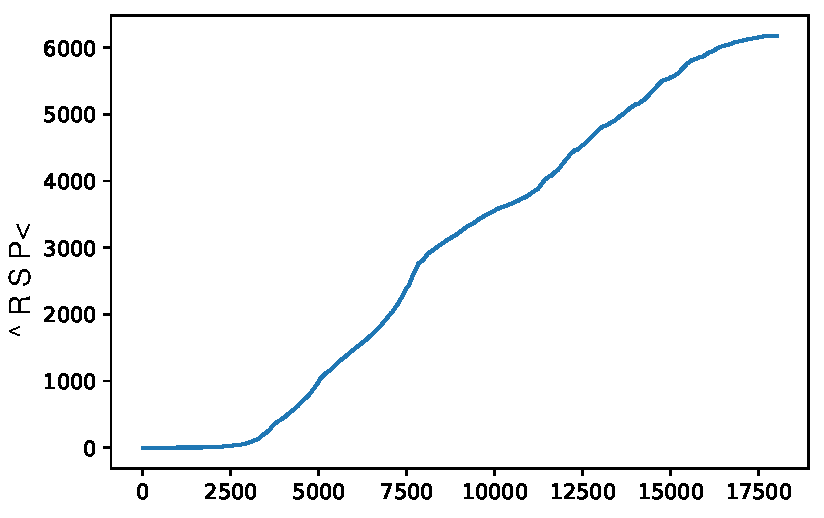
\includegraphics[width=1\textwidth]{Img/chapter11/flock-martingale-MLPClassifier}   
         \caption{Flock数据集的复合跳跃鞅}
         \label{mlp-jump-flock}
     \end{subfigure}
     \hfill
     \begin{subfigure}[b]{.45\textwidth}
         \centering
         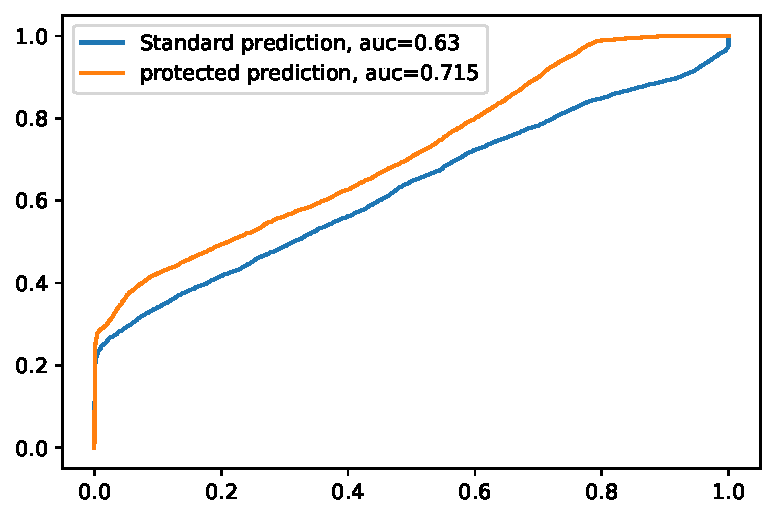
\includegraphics[width=1\textwidth]{Img/chapter11/flock-MLPClassifier}
         \caption{Flock数据集鞅保护分布算法结果}
         \label{mlp-jump-martingale-flock}
     \end{subfigure}
\caption{Flock数据集的复合跳跃鞅以及鞅保护分布算法结果}
\label{fig:flock}
\end{figure}

对于Group数据集, 图 \ref{mlp-jump-group} 给出的是复合鞅序列, 同样可以看到Group数据集也发生分布漂移。 利用这种分布变化, 基于鞅保护分布算法校正底层神经网络算法。 图\ref{mlp-jump-martingale-group} 给出校正后的ROC得分比较。 很明显, 通过鞅保护分布算法针对Group数据集分类指标AUC由神经网络算法的0.715提升至0.789。

%\begin{figure} % [tb]
%\begin{center}
%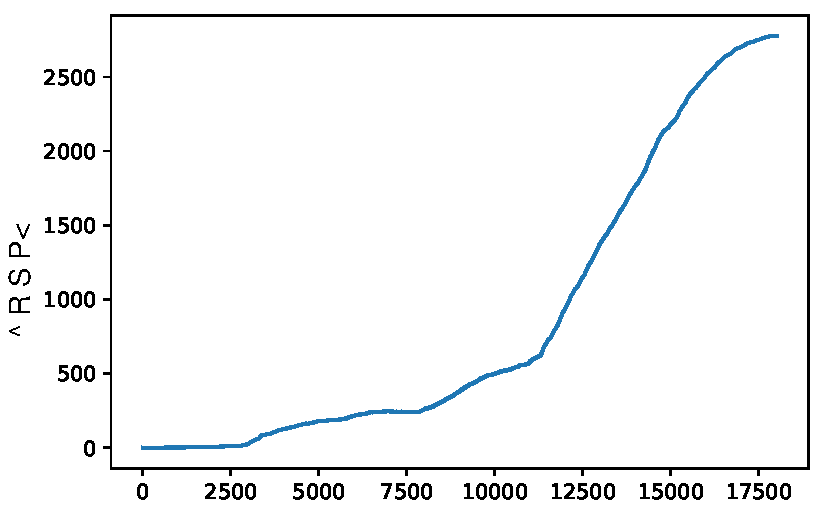
\includegraphics[width=0.4\textwidth]{Img/chapter11/group-martingale-MLPClassifier}
%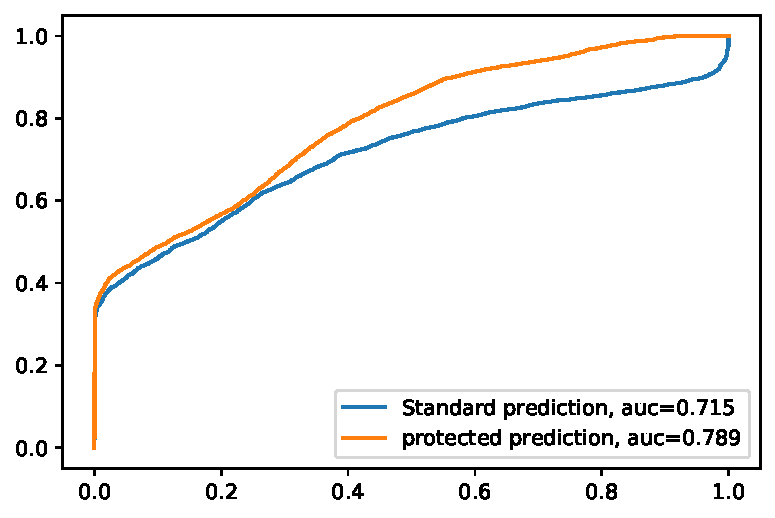
\includegraphics[width=0.4\textwidth]{Img/chapter11/group-MLPClassifier}
%\end{center}
%\caption{Group数据集的复合跳跃鞅以及鞅保护分布算法结果}
%\label{fig:group}
%\end{figure}

\begin{figure}
     \centering
     \begin{subfigure}[b]{.45\textwidth}
         \centering
         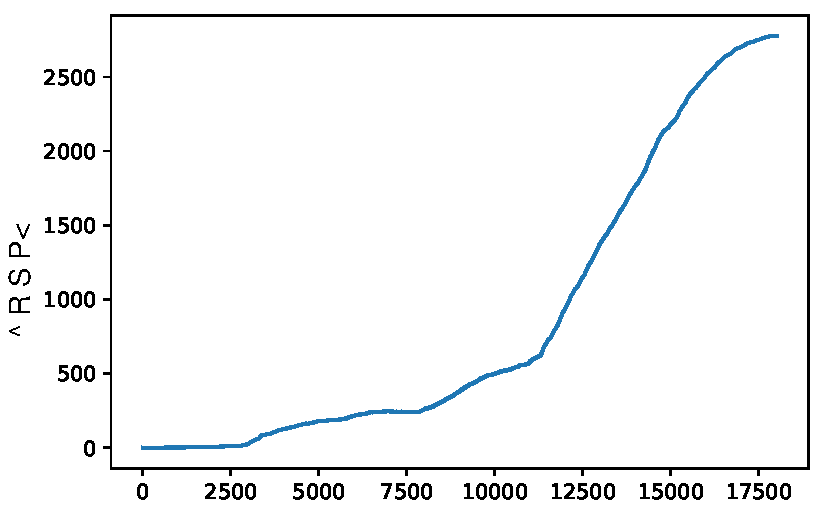
\includegraphics[width=1\textwidth]{Img/chapter11/group-martingale-MLPClassifier}   
         \caption{Group数据集的复合跳跃鞅}
         \label{mlp-jump-group}
     \end{subfigure}
     \hfill
     \begin{subfigure}[b]{.45\textwidth}
         \centering
         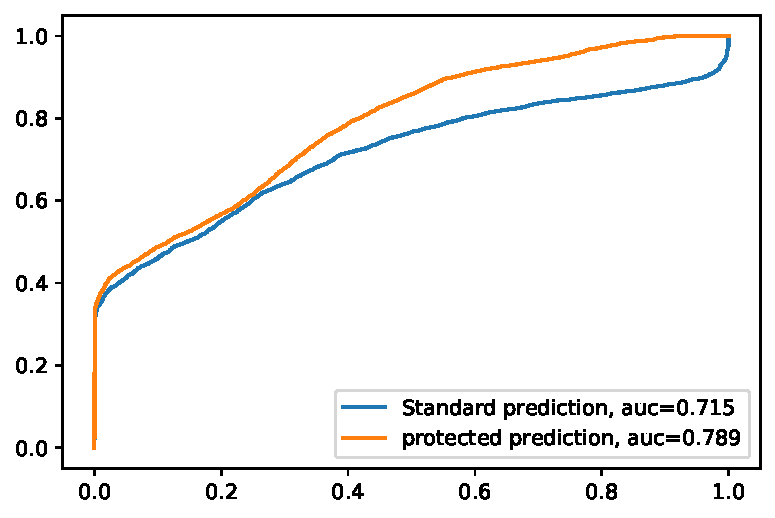
\includegraphics[width=1\textwidth]{Img/chapter11/group-MLPClassifier}
         \caption{Group数据集鞅保护分布算法结果}
         \label{mlp-jump-martingale-group}
     \end{subfigure}
\caption{Group数据集的复合跳跃鞅以及鞅保护分布算法结果}
\label{fig:group}
\end{figure}

为了和第\ref{chapter:swarm-distributions}章中讨论的结果比较, 本章给出有序学习下三种无人机集群错误分类数目的统计对比。表\ref{tab:align-num-martingale}给出Align数据集鞅保护分布算法预测错误数目与第\ref{chapter:swarm-distributions}章中表\ref{tab:online}的对比结果。从表\ref{tab:align-num-martingale}可知, 采用鞅保护分布算法能够明显降低错误分类的数目。例如, 经过鞅保护分布算法, 对于Align数据集可以将第\ref{chapter:swarm-distributions}章中表\ref{tab:online}采用SVMs算法分类错误数目由1492降低到1347, 降幅9.72\%; 将采用神经网络算法分类错误数目由848降低到665, 降幅21.58\%; 将采用Boosting算法分类错误数目由1763降低到1477, 降幅16.22\%。

% Please add the following required packages to your document preamble:
% \usepackage{booktabs}
% \usepackage{graphicx}
\begin{table}[]
\centering
\caption{Align数据集鞅保护分布算法预测错误数目对比}
\label{tab:align-num-martingale}
\begin{tabular}{@{}llll@{}}
\toprule
预测算法类别   & 无保护时错误数目(表\ref{tab:online}) & 鞅保护后错误数目 & 提升百分比 \\ \midrule
SVMs     & 1492          & \textbf{1347}      &       {9.72\%}\\
神经网络     & 848           & \textbf{665}      &     {21.58\%} \\
Boosting & 1763          & \textbf{1477}     &       {16.22\%} \\ \bottomrule
\end{tabular}%
\end{table}

表\ref{tab:flock-num-martingale}给出Flock数据集鞅保护分布算法预测错误数目与第\ref{chapter:swarm-distributions}章中表\ref{tab:online}的对比结果。对于Flock数据集可以将第\ref{chapter:swarm-distributions}章中表\ref{tab:online}采用神经网络算法分类错误数目由2125降低到1876, 降幅11.72\%; 将采用Boosting算法分类错误数目由2055降低到1742, 降幅15.23\%; 但是对于采用SVMs算法却没有给出提升效果。

% Please add the following required packages to your document preamble:
% \usepackage{booktabs}
% \usepackage{graphicx}
\begin{table}[]
\centering
\caption{Flock数据集鞅保护分布算法预测错误数目对比}
\label{tab:flock-num-martingale}
\begin{tabular}{@{}llll@{}}
\toprule
预测算法类别   & 无保护时错误数目(表\ref{tab:online}) & 鞅保护后错误数目 & 提升百分比 \\ \midrule
SVMs     & \textbf{2928}          & 3027      &       {-3.38\%}\\
神经网络     & 2125           & \textbf{1876}      &     {11.72\%}  \\
Boosting & 2055          & \textbf{1742}     &       {15.23\%} \\ \bottomrule
\end{tabular}%
\end{table}


表\ref{tab:group-num-martingale}给出Group数据集鞅保护分布算法预测错误数目与第\ref{chapter:swarm-distributions}章中表\ref{tab:online}的对比结果。对于Group数据集可以将第\ref{chapter:swarm-distributions}章中表\ref{tab:online}采用神经网络算法分类错误数目由1031降低到942, 降幅8.63\%; 将采用Boosting算法分类错误数目由452降低到401, 降幅11.28\%; 但是对于采用SVMs算法却没有给出提升效果。

% Please add the following required packages to your document preamble:
% \usepackage{booktabs}
% \usepackage{graphicx}
\begin{table}[]
\centering
\caption{Group数据集鞅保护分布算法预测错误数目对比}
\label{tab:group-num-martingale}
\begin{tabular}{@{}llll@{}}
\toprule
预测算法类别   & 无保护时错误数目(表\ref{tab:online}) & 鞅保护后错误数目 & 提升百分比 \\ \midrule
SVMs     & \textbf{1385}          & 1421      &      {-2.60\%} \\
神经网络     & 1031           & \textbf{942}      &   {8.63\%}   \\
Boosting & 452          & \textbf{401}     &      {11.28\%} \\ \bottomrule
\end{tabular}%
\end{table}


同样的, 也可以针对其他不同机器学习算法对比鞅保护分布算法的效果。分别选择 SVMs, 神经网络, 决策树模型, 随机森林, 朴素贝叶斯和逻辑回归等六种机器学习作为底层算法, 检验采用鞅保护前后的泛化推广能力。 为了统一比较算法, 本次对比选择更常用的AUC值作为评价指标。

表 \ref{tab:align} 展示的是针对Align数据集, 这六种学习算法在采用鞅保护前后的预测能力。 从表中可以看到, 对于Align数据集, 鞅保护后的算法比未经鞅保护的底层算法预测能力都得到提高。 例如, 对于常规SVMs算法, 其对于Align行为分类效果的AUC值为0.654, 采用鞅保护分布算法得到的AUC值提升至 0.732; 对于常规神经网络算法, 其对于Align行为分类效果的AUC值为0.517, 采用鞅保护分布算法得到的AUC值提升至 0.724; 对于常规决策树模型算法, 其对于Align行为分类效果的AUC值为0.508, 采用鞅保护分布算法得到的AUC值提升至 0.641; 对于常规随机森林算法, 其对于Align行为分类效果的AUC值为0.604, 采用鞅保护分布算法得到的AUC值提升至 0.722; 对于常规朴素贝叶斯算法, 其对于Align行为分类效果的AUC值为0.460, 采用鞅保护分布算法得到的AUC值提升至 0.650; 对于常规逻辑回归算法, 其对于Align行为分类效果的AUC值为0.440, 采用鞅保护分布算法得到的AUC值提升至 0.710。 并且通过这种对比可以看到, 鞅保护分布算法对于基于模型假定的传统统计学范式(朴素贝叶斯和逻辑回归模型)的提升能力是相当明显可观的。 

% Please add the following required packages to your document preamble:
% \usepackage{booktabs}
\begin{table}[]
\centering
\caption{Align数据集鞅保护分布算法对比汇总表}
\label{tab:align}
\begin{tabular}{@{}llll@{}}
\toprule
预测算法类别 & 无保护时AUC值 & 鞅保护后AUC值 & 提升百分比 \\ \midrule
SVMs                & 0.654     & \textbf{0.732}  &  {10.66\%}  \\
神经网络       & 0.517     & \textbf{0.724}  &  {28.59\%}  \\
决策树        & 0.508     & \textbf{0.641}  &  {20.75\%} \\
随机森林        & 0.604     & \textbf{0.722}  &  {16.34\%} \\
朴素贝叶斯     & 0.460     & \textbf{0.650}  &  {29.23\%}  \\
逻辑回归  & 0.440     & \textbf{0.710}  &  {38.03\%}  \\ \bottomrule
\end{tabular}
\end{table}

表 \ref{tab:flock} 给出针对 Flock 数据集的预测效果对比。 从表中可以看到, 对于常规SVMs算法, 其对于Flock行为分类效果的AUC值为0.749, 采用鞅保护分布算法得到的AUC值降低为 0.721; 对于常规神经网络算法, 其对于Flock行为分类效果的AUC值为0.630, 采用鞅保护分布算法得到的AUC值提升至 0.715; 对于常规决策树模型算法, 其对于Flock行为分类效果的AUC值为0.654, 采用鞅保护分布算法得到的AUC值提升至 0.703; 对于常规随机森林算法, 其对于Flock行为分类效果的AUC值为0.707, 采用鞅保护分布算法得到的AUC值提升至 0.814; 对于常规朴素贝叶斯算法, 其对于Flock行为分类效果的AUC值为0.627, 采用鞅保护分布算法得到的AUC值提升至 0.687; 对于常规逻辑回归算法, 其对于Flock行为分类效果的AUC值为0.598, 采用鞅保护分布算法得到的AUC值提升至 0.694。 当然在Flock数据集上, 鞅保护分布算法对于SVMs算法并没有带来分类能力的提升, 反而降低其AUC值。 这是因为对于SVMs算法, 由于其本身属于超越推理模型, 其输出值并不来自最外层固定的具体函数。 因此可以理解为什么在Flock数据集上鞅保护分布算法对SVMs给出相反的结论。

% Please add the following required packages to your document preamble:
% \usepackage{booktabs}
\begin{table}[]
\centering
\caption{Flock数据集鞅保护分布算法对比汇总表}
\label{tab:flock}
\begin{tabular}{@{}llll@{}}
\toprule
预测算法类别 & 无保护时AUC值 & 鞅保护后AUC值 & 提升百分比 \\ \midrule
SVMs                 & \textbf{0.749}        & 0.721      		 & {-3.88\%}\\
神经网络       & 0.630                 & \textbf{0.715}      & {11.89\%}\\
决策树        & 0.654                 & \textbf{0.703}      & {6.67\%}\\
随机森林        & 0.707                 & \textbf{0.814}      & {13.14\%}\\
朴素贝叶斯     & 0.627                 & \textbf{0.687}      & {8.73\%}\\
逻辑回归  & 0.598                 & \textbf{0.694}      & {13.83\%}\\ \bottomrule
\end{tabular}
\end{table}

鞅保护分布算法为底层机器学习算法带来的提升在Group数据集上也具有明显的提升效果。 表 \ref{tab:group} 展示的是这六种算法以及对应的鞅保护分布算法对Group行为数据集学习效果提升的对比。从表中可以看到, 对于常规SVMs算法, 其对于Group行为分类效果的AUC值为0.827, 采用鞅保护分布算法得到的AUC值降低为 0.809; 对于常规神经网络算法, 其对于Group行为分类效果的AUC值为0.715, 采用鞅保护分布算法得到的AUC值提升至 0.789; 对于常规决策树模型算法, 其对于Group行为分类效果的AUC值为0.545, 采用鞅保护分布算法得到的AUC值提升至 0.654; 对于常规随机森林算法, 其对于Group行为分类效果的AUC值为0.686, 采用鞅保护分布算法得到的AUC值提升至 0.784; 对于常规朴素贝叶斯算法, 其对于Group行为分类效果的AUC值为0.693, 采用鞅保护分布算法得到的AUC值提升至 0.746; 对于常规逻辑回归算法, 其对于Group行为分类效果的AUC值为0.731, 采用鞅保护分布算法得到的AUC值提升至 0.789。 同样的, 在Group行为数据集合上, 鞅保护分布算法对于SVMs模型并没有给出提升的效果, 但是对于其他机器学习算法, 其均给出令人满意的结果。

% Please add the following required packages to your document preamble:
% \usepackage{booktabs}
\begin{table}[]
\centering
\caption{Group数据集鞅保护分布算法对比汇总表}
\label{tab:group}
\begin{tabular}{@{}llll@{}}
\toprule
预测算法类别 & 无保护时AUC值 & 鞅保护后AUC值 & 提升百分比\\ \midrule
SVMs                 & \textbf{0.827}        & 0.809               & {-2.22\%}\\
神经网络      & 0.715                 & \textbf{0.789}      & {9.38\%}\\
决策树       & 0.545                 & \textbf{0.654}      & {16.67\%}\\
随机森林        & 0.686                 & \textbf{0.784}      & {12.50\%}\\
朴素贝叶斯     & 0.693                 & \textbf{0.746}      & {7.10\%}\\
逻辑回归  & 0.731                 & \textbf{0.789}      & {7.35\%}\\ \bottomrule
\end{tabular}
\end{table}
 
\section{本章小结}
\label{conclusion}
本章以无人机集群行为数据本身的时间顺序为研究对象, 针对考虑数据自身时间顺序的无人机集群行为分类问题进行研究。主要结论总结如下:
\begin{enumerate}
\item 针对实际工程应用中数据可能出现的分布漂移现象, 构建新的分布漂移检测指标。这种新检测指标同样也能够高效地给出分布漂移的证据;
\item 提出一种鞅保护分布框架提升底层机器学习算法的性能。鞅保护分布算法建立在机器学习算法顶层, 可以为大多数机器学习算法的预测效果提供明显的改进;
\item 本节提出的算法不仅仅指出实际数据中会出现的分布漂移现象, 而且将数据本身的分布信息融合至底层学习算法, 说明数据本身的时间顺序是不可被忽视的信息。
\end{enumerate}
\chapter{使用特权信息学习范式的无人机集群行为分类研究}
\label{chap:intelligent-learning}

\section{引言}
自Vapnik和Chervonenkis提出模式识别理论后\citep{vapnik1974}, 强机器学习理论的知识已经被建立起来 \citep{vapnik1974,vapnik1979,vapnik1982,vapnik1995,vapnik1998,Vapnik2006,Chervonenkis2013}。第\ref{chap:edbed}章给出的也是强机器学习理论一致收敛的充分必要条件, 根据第\ref{chap:edbed}章的研究内容, 强机器学习理论已经解决如下关于机器学习的基础问题:
\begin{enumerate}
\item 学习过程收敛的充分必要条件(第\ref{sec:uniform-convergence}节给出),
\item 学习过程收敛的速度的界(第\ref{sec:rate-of-convergence}节给出),
\item 基于容量控制的一种新归纳推理原则——结构风险最小化原则——通过控制两个因素(即最小化经验风险泛函和容量)使得学习模型总是收敛至最优的逼近函数(第\ref{sec:special-case}给出),
\item 开发的SVMs算法实现结构风险最小化原则。
\end{enumerate}

因此关于一般学习理论的研究似乎完成: 因为以上四个问题几乎在理论上完整回答所有与统计推理相关的问题, 剩下的只是一些修修补补。 例如用第\ref{chap:Swarm-MCP}章提出的一致性预测为机器学习算法输出给出一些可信程度的度量; 用第\ref{chapter:swarm-distributions}章介绍的无分布假设的鞅方法提供分布漂移检测并且当发生分布漂移时重新训练模型即可; 或者根据第\ref{chapter:swarm-martingales}章介绍的鞅保护分布方法提升机器学习的预测能力。虽然上述章节提出的方法在一定程度上能够提供一些改进, 但是确切说来这些改进都建立在第\ref{chap:edbed}章的研究内容之上。所以从理论层面而言, 似乎的确关于一般学习理论的研究已然完成。

然而, 核心问题总藏在理论阐述的细节之处\citep{Vapnik-similary-2015,Vapnik2021}。通过对比人类学习和机器学习之后就不难发现, 人类学习所需要的样本要比机器学习少得多。在前面章节的模型构建中, 大都需要上千个训练样本才能得到相对令人满意的结果, 但是显然对于人类而言并不需要太多的样本就可以完成相当不错的学习。从提供学习一致性收敛的VC理论来看, 第\ref{chap:edbed}章的研究已经表明, 学习一致收敛依赖于两个因素: 即一方面取决于分类规则将下列训练数据分开的质量
\begin{align}
\label{ch4:train-data}
(x_{1}, y_{1}), \ldots, (x_{l}, y_{l}), x \in R^{n}, y \in \{-1, +1\},
\end{align}
另一方面取决于被选中的规则所在的诸函数的集合本身的VC维。

形式化而言, VC理论有两种明显不同的情形:
\begin{enumerate}
\item[1.] \textsf{对于可分情形:} 根据第\ref{chap:edbed}章中第\ref{sec:kefen}节的内容, 这种情形下在具有有限VC维$h$的诸函数$f(x,\alpha), \alpha \in \Lambda$的集合中, 存在一个函数$f(x,\alpha_{l})$其能够将训练数据 (\ref{ch4:train-data})完全正确地分开, 即
\begin{align}
y_{i}f(x_{i}, \alpha_{l}) > 0, \forall i = 1, \ldots, l.
\end{align}
在这种可分情形下, 一致收敛的速度的界
\begin{align}
P(yf(x, \alpha_{l}) \leq 0) < O^{*}\left(\frac{h - \ln \eta}{l}\right)
\end{align}
以概率 (with probability) $1-\eta$ 成立。 其中, 这里$P(yf(x, \alpha_{l}) \leq 0)$是函数$f(x, \alpha_{l})$错误分类的概率, $h$是诸函数可行集的VC维, 标识符$O^{*}$表示的是对数因子高阶项的阶数。
\item[2.] \textsf{对于不可分情形:} 根据第\ref{chap:edbed}章中第\ref{sec:special-case}节的内容, 这种情形下在具有有限VC维$h$的诸函数$f(x,\alpha), \alpha \in \Lambda$的集合中, 不存在函数能够将训练数据 (\ref{ch4:train-data})完全正确地分开。 因此, 设$f(x, \alpha_{l})$是在训练集(\ref{ch4:train-data})上最小化分类错误数目的函数, 令$v(\alpha_{l})$是此函数在训练集上的错误频率。那么根据VC理论, 下列一致收敛的速度的界
\begin{align}
P(yf(x, \alpha_{l}) \leq 0) < v(\alpha_{l}) + O^{*}\left(\sqrt{\frac{h - \ln \eta}{l}}\right)
\end{align}
以概率 (with probability) $1-\eta$ 成立。
\end{enumerate}

也就是说, 在可分情形下一致收敛的速度的界具有$O(\frac{1}{l})$的阶数; 而在不可分情形下一致收敛的速度的界具有$O(\frac{1}{\sqrt{l}})$的阶数。 换言之, 这表明为获得相同阶数的收敛, 在可分情形下只要$100$个样本而在不可分情形下则需要$100^{2} = 10000$个样本。 

为什么根据VC理论, 可分情形和不可分情形需要的样本数目会产生如此这般巨大的差别, 这种差别正就类似于人类学习和机器学习之间的差别。Vapnik认为人类学习和机器学习之间产生差距的原因在于“人类实现快速学习的原因是因为人类有老师的指导”\citep{vapnikinterview2014,vapniktalk2022,vapniktalk2022-02}, 能够在VC维对知识本身展开学习\citep{Vapnik-rethinking-2018,vapnik2020,Vapnik2021,2019Reconciling}。 使用特权信息学习 (Learning Using Privileged Information, LUPI)\citep{Vapnik2009,vapnik2015}模型基于这一思想出发, 可以提供在小样本下实现高精度的学习范式。

本章首先介绍LUPI方法的相关研究, 然后基于LUPI方法提出使用整体描述信息作为特权信息加速学习算法的收敛速度, 构建在两种不同类型的整体描述信息下无人机集群行为分类的LUPI学习范式, 进而将提出的方法应用于三种公开无人机集群行为数据集。最后, 通过数值算例对所提方法的可行性和有效性进行验证。


\section{使用特权信息学习方法的理论研究}
本节首先解释为什么在可分情形和不可分情形下学习算法的收敛速度会产生如此大的差距。

利用SVMs来说明这一问题。SVMs首先将空间$X$的向量$x$映射至空间$Z$中的向量$z$, 然后在空间$Z$构建分隔超平面。 对于可分情形, SVMs最小化下列泛函
\begin{align}
\mathcal{T}(w) = (w, w)
\end{align}
其约束条件是
\begin{align}
(y_{i}((w, z_{i}) + b)) \geq 1, \forall i = 1, \ldots, l;
\end{align}
而对于不可分情形, SVMs最小化下列泛函
\begin{align}
\mathcal{T}(w) = (w, w) + C\sum_{i=1}^{l}\xi_{i}
\end{align}
其约束条件是
\begin{align}
(y_{i}((w, z_{i}) + b)) \geq 1 - \xi_{i}, \forall i = 1, \ldots, l;
\end{align}
其中, 这里的$\xi_{i} \geq 0$ 都是松弛变量。 这就是说, 在可分情形下SVMs使用$l$个样本估计向量$w$的$N$个系数; 而在不可分情形下SVMs使用$l$个样本估计$N+l$个系数——向量$w$的$N$个系数和松弛变量$\xi_{i}$的$l$个取值。 因此, 在不可分情形下需要估计的参数个数$N+l$始终大于样本数$l$。 因为松弛变量大多取值为0并不会影响这种局面, 所以可能是SVMs需要估计的参数个数造成这种差距。

现在考虑伴随神谕老师(Oracle Teacher)的SVMs。 假设老师能先入之见地提供给学生诸松弛变量取值(将这些“先入之见的信息”称为“特权信息”\citep{Husser1928,Husser1948-en}), 那么在训练阶段, 就可以拥有下列三元组数据
\begin{align}
(x_{1}, \xi_{1}^{0}, y_{1}), \ldots, (x_{l}, \xi_{l}^{0}, y_{l}),
\end{align}
其中, 这里$\xi_{i}^{0}, i = 1, \ldots, l$是所有贝叶斯决策规则的松弛变量。 因此, 为构建决策规则, SVMs必须最小化下列泛函
\begin{align}
\mathcal{T}(w) = (w, w)
\end{align}
其约束条件是
\begin{align}
y_{i}((w, z_{i}) + b) \geq r_{i}, \forall i = 1, \ldots, l,
\end{align}
其中, 这里
\begin{align}
r_{i} = 1 - \xi_{i}^{0}, \forall i = 1, \ldots, l.
\end{align}
因为有神谕老师能够提供贝叶斯决策规则的松弛变量, 原本不可分的问题转变为可分问题, 收敛速率就等于$O^{*}(\frac{1}{l})$。\citet{Vapnik2009}证明神谕老师范式下学习的收敛速率。
\begin{proposition}\citep{Vapnik2009}
设$f(x, \alpha_{0})$是来自于VC维为h的诸示性函数$f(x,\alpha), \alpha \in \Lambda$的集合的函数, 此函数能够最小化分类错误的频率, 令
\begin{align}
\xi_{i}^{0} = \max \{0, 1-f(x_{i}, \alpha_{0})\}, \forall i = 1, \ldots, l.
\end{align}
那么对于满足下列约束条件
\begin{align}
y_{i}f(x_{i}, \alpha_{l}) \geq 1 - \xi_{i}^{0}, \forall i = 1, \ldots, l
\end{align}
的函数$f(x, \alpha_{l})$的概率$p(\alpha_{l})$是以概率 (with probability) $1 - \eta$界住, 即
\begin{align}
p(\alpha_{l}) \leq P(1 - \xi^{0} < 0) + O^{*}\left( \frac{h - \ln \eta}{l}\right).
\end{align}
\end{proposition}

LUPI学习范式通过引进特权信息——这种信息只能够在训练阶段有用而无法在测试阶段使用——来加速学习问题的收敛速度。在近期研究中, \citet{Vapnik-similary-2015,vapnik2015}揭示通过知识转化可以得到LUPI的稳定求解, 这种方法将学习模型的输出作为特权信息。\citet{Shiao2014} 将LUPI学习范式应用于生存数据建模, 提出一种基于LUPI范式的生存数据模型, 根据LUPI学习范式可以方便地将统计学中难以处理的生存数据切分为常规输入和特权信息输入, 进而获得高效的求解。\citet{Vrigkas2017}基于LUPI范式开发出一种提供现代新型人机交互识类型的识别算法, 研究者可以提供丰富的特权信息以加速识别算法的收敛。\citet{Izmailov2017}则考虑将LUPI应用于特征选择问题中, 他们将只能在训练阶段可用而在测试阶段不可用的特征作为特权信息, 以此基于LUPI范式实现高效的特征选择。 \citet{Izmailov2018} 将LUPI特征选择方法改进为一种自动特征选择方法, 这种LUPI类型算法不仅能够实现特征选择自动化, 而且能够充分利用潜在数据扩大备选特征的规模, 进而提高整体模型的预测效果。

根据文献调研, 鲜有在无人机集群领域中关注到LUPI类型的学习范式, 提出将无人机集群数据中的整体描述信息作为特权信息, 并构建LUPI模型加速底层学习算法的收敛速度。

\section{无人机集群使用特权信息学习方案设计}
\label{sec:swarm-behavior-empirical}

对于无人机集群行为分类问题, 当前的研究大都将之归约为监督学习问题, 然后借用机器学习算法逼近最优函数。 例如\citet{Tunstrm2013} 指出通过使用排序后的参数集合可以描述集群的机动结构。 \citet{Michael2014} 则报告针对大规模仿真机器智能体的自组织系统, 其通过成百上千个智能体通过彼此之间的信息交互就可以形成高度复杂的集群行为。 \citet{Brown-Human-swarm2014} 使用高阶吸引子集群模型来管理集群系统的整体行为。\citet{Brown2014} 则给出一种用于集群分类的创新框架, 这种框架通过使用局部近似模型来区分两种仿生集群行为。 \citet{Walker2014}则利用高斯模型来重建集群行为模式, 特别地, 在这篇文章中作者是采用集群个体的速度场作为模型输入, 然后通过高斯过程模型来实现集群行为的分类。\citet{Berger2016} 提出一种压缩子空间方法求解集群行为分类。 他们将单个智能体的速度域数据作为模型输入, 通过借用SVMs将之映射至低维数空间来实现集群行为的分类。

所有这些已发表的文献其实都希望借用机器学习方法实现复杂集群行为的分类, 并且从理论上分析可知这些研究都可以被归约为模式识别问题来处理。 从形式上看可表述为给定下列数据对 
\begin{align}
(x_{1}, y_{1}), \ldots, (x_{l}, y_{l}), \quad x_{i} \in X, y_{i} \in \{-1, 1\},
\end{align}
假设这些数据对是根据某个固定的、但是未知的概率测度$P(x,y) = P(y|x)P(x)$生成的。 机器学习算法在给定的诸示性函数的集合$f(x,\alpha), \alpha \in \Lambda$——诸示性函数的集合是由机器实现的——中找一个函数$y = f(x, \alpha_{0})$, 此函数能够最小化错误分类的个数。 在无人机集群行为分类问题中, 这里的输入向量$x_{i} \in X$由位置域组成, 而$y_{i} \in \{-1, 1\}$就是无人机集群整体对应的标签。

然而, 在构建学习算法时不仅仅局限在上述已经给出的数据集, 研究者对数据集本身的直观描述也是可用的。 的确, 对于集群行为分类问题而言, 在训练阶段不仅仅位置域信息可用, 而且一些额外的信息也是可以获得的。 比如, 在训练阶段是能够获取智能体彼此之间的交互信息的, 但是这种交互信息仅仅在训练数据集上可以获得, 无法在测试数据集上使用。 因此, 考虑如何将这种额外信息与现有模型融合, 进而期待能够加速学习收敛速率。 形式化而言, 考虑使用LUPI范式来处理集群行为分类任务, 这种学习范式给定三元组数据集合
\begin{align}
(x_{1}, x_{1}^{*}, y_{1}), \ldots, (x_{l}, x_{l}^{*}, y_{l}), \quad x_{i} \in X, x_{i}^{*} \in X^{*}, y_{i} \in \{-1,1\},
\end{align}
此三元组数据是由固定的、但是未知的概率分布$P(x,x^{*},y) = P(y, x^{*} | x)P(x)$生成。 现在的问题是在给定的诸示性函数$f(x,\alpha), \alpha \in \Lambda$集合中——诸示性函数集合由机器实现——找到一个函数$y = f(x, \alpha_{0})$, 此函数能够最小化错误分类的数目。 在这个模型中, 假设向量$x_{i} \in X$是由某固定的、但是未知的概率分布$P(x)$生成, 输入变量不仅仅是无人机集群对应的标签$y_{i} \in \{-1, 1\}$, 同时也提供特权信息$x_{i}^{*} \in X^{*}$, 此特权信息服从未知的条件概率函数$P(y_{i},x_{i}^{*} | x_{i})$。 例如, 在集群行为分类问题中的特权信息$x_{i}^{*} \in X^{*}$可以是由人类提供的某种整体描述, 并且这种整体描述仅仅在训练阶段可用。


针对处理复杂无人机集群行为识别问题, 提出考虑将人机交互信息——即人对于输入数据的整体描述——通过LUPI范式实现知识转换。 引进两种类型的特权信息, 其一是对整个无人机集群的整体合作描述, 其二是智能体彼此之间的内在竞争信息。 

图 \ref{fig:demo}展示在无人机集群的整体合作描述下的LUPI学习范式。如图所示, 训练阶段的输入不仅仅包含常规位置域信息(分别展示Align行为, Torus行为和Random行为等), 而且还包括特权信息(这些特权信息分别表示为Align*, Torus*和Random*)。不同的集群行为对应不同的特权信息$X^{*}$。所有的特权信息仅仅在训练阶段可用, 在测试阶段无法使用。因此, 一旦LUPI模型训练完成, 在测试阶段仅将常规位置域信息输入LUPI模型来获得对应的预测结果。

\begin{figure*}
\centering
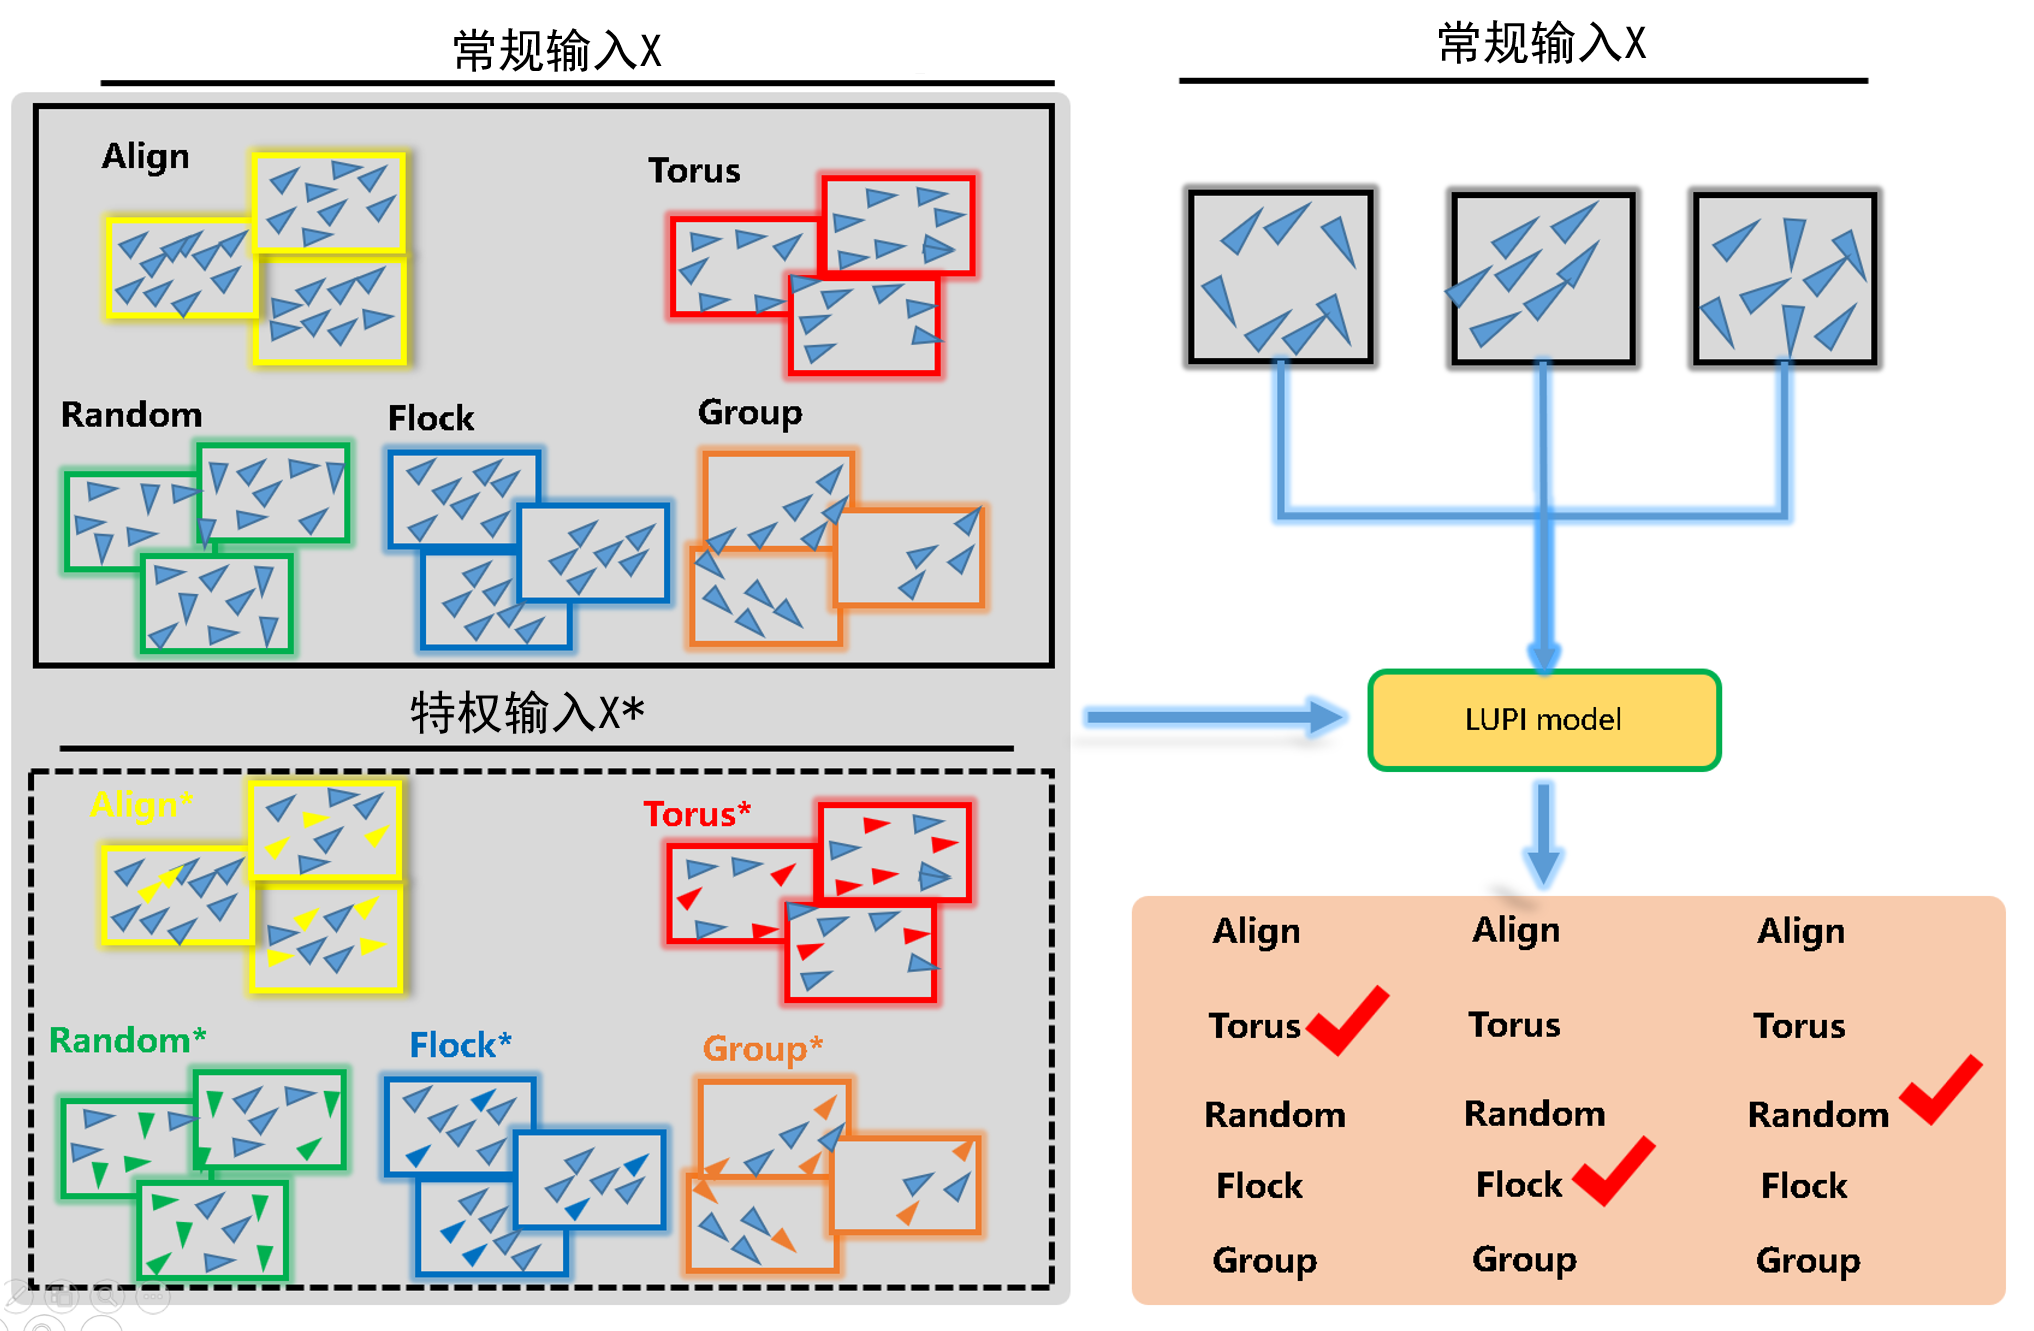
\includegraphics[width=1\textwidth]{Img/chapter10/LUPI.png}
\caption{使用特权信息学习范式方案设计框架图}
\label{fig:demo}
\end{figure*}

为学习所求的决策函数$y = f(x)$, LUPI方法首先将决策空间$X$中的向量$x$映射至特征空间$Z$中的向量$z$, 将特权空间$X^{*}$中的向量$x^{*}$映射至特征空间$Z^{*}$中的特征向量$z^{*}$, 在特征空间构建最优分隔超平面。 形式化的表述, 即考虑最小化下列泛函
\begin{align}
R(w, w^{*}, b, b^{*}) = \frac{1}{2}[(w, w) + \gamma (w^{*}, w^{*})] + C\sum_{i=1}^{l}[(w^{*}, z_{i}^{*}) + b^{*}]
\end{align}
其约束条件是
\begin{align}
&y_{i}[(w, z_{i}) + b] \geq 1 - [(w^{*}, z_{i}^{*}) + b^{*}], \quad i = 1, \ldots, l,\\
&[(w^{*}, z_{i}^{*}) + b^{*}] \geq 0, \quad i= 1, \ldots, l.
\end{align}

为求解此优化问题, 考虑其对应的Lagrangian乘子
\begin{equation}
\begin{aligned}
L(w, b, w^{*}, b^{*}, \alpha, \beta) &= \frac{1}{2}[(w, w) + \gamma (w^{*}, w^{*})] + C\sum_{i=1}^{l}[(w^{*}, z_{i}^{*}) + b^{*}]\\
& - \sum_{i=1}^{l}\alpha_{i}\left[y_{i}[(w, z_{i}) + b] - 1 + [(w^{*}, z_{i}^{*}) + b^{*}]\right]\\
& - \sum_{i=1}^{l}\beta_{i}\left[(w^{*}, z_{i}^{*}) + b^{*}\right]
\end{aligned}
\end{equation}
针对$w,b,w^{*},b^{*}$求此Lagrangian的最小化, 针对Lagrangian算子$\alpha \geq 0, \beta \geq 0$求此Lagrangian的最大化。

通过求解下列对偶问题可得LUPI问题的解, 即最大化下列泛函
\begin{equation}
\begin{aligned}
R(\alpha, \beta) &= \sum_{i=1}^{l}\alpha_{i} - \frac{1}{2}\sum_{i,j=1}^{l}\alpha_{i}\alpha_{j}y_{i}y_{j}(z_{i},z_{j})\\
& - \frac{1}{2\gamma}\sum_{i,j=1}^{l}(\alpha_{i} + \beta_{i} - C)(\alpha_{j} + \beta_{j} - C)(z_{i}^{*}, z_{j}^{*})
\end{aligned}
\end{equation}
其约束条件是
\begin{align}
&\sum_{i=1}^{l}(\alpha_{i} + \beta_{i} - C) = 0,\\
&\sum_{i=1}^{l}y_{i}\alpha_{i} = 0,\\
&\alpha_{i} \geq 0, \beta_{i} \geq 0, i = 1,\ldots,l.
\end{align}
其中, 这里 $(z_{i},z_{j}) = K(x_{i}, x_{j})$ 并且 $(z_{i}^{*}, z_{j}^{*}) = K^{*}(x_{i}^{*}, x_{j}^{*})$ 分别是在空间 $X$ 和空间 $X^{*}$上的核函数。

根据Vapnik-Chervonenkis理论\citep{Vapnik2006}, 此问题的解 $(w,b)$ 定义的分类超平面在\textsf{不可分情形}下的错误率\textsc{以概率} (with probability) $1-\eta$ 的界为
\begin{align}
P_{test} \leq v_{train} + O^{*}(\sqrt{\frac{VCdim}{l}}),
\end{align}
然而, 如果给定某三元组序列中的特权信息$x_{i}^{*}, i=1,\ldots,l$都是针对那最优超平面的理想变量 (ideal variables)的话——此时就将\textsf{不可分问题}转变为\textsf{可分问题}——那么此问题的解 $(w,b)$ 所定义的分类超平面的错误率就\textsc{以概率} (with probability) $1-\eta$被下列表达式界住
\begin{align}
P_{test} \leq v_{train} + O^{*}(\frac{VCdim}{l}).
\end{align}


采集的数据集仍然是根据公开发表在UC Irvine 机器学习数据仓库上的无人机集群行为数据集。 这一数据由澳大利亚新南威尔士大学托管的一个在线调查获得, 此数据包含三种行为数据集, 分别是\texttt{Flock}行为, \texttt{Align}行为和 \texttt{Group}行为。 在线调查的数据本身也是基于某无人机集群行为模型, 但是其标签是由参加在线调查的用户标记。 第\ref{chap:Swarm-MCP}章的表 \ref{tab:datainfo} 汇总介绍真实集群行为数据集的概要信息, 这些属性参见第\ref{chap:Swarm-MCP}章第\ref{sec:truth-swarm}节中的介绍。

现在介绍针对无人机集群行为识别如何在技术上落地LUPI学习范式。 无人机集群行为预测的核心问题是将无人机集群整体刻画作为特权信息, 本文拟提供两种整体性描述信息来加速计算机识别的收敛速度。在本文中所谓“加速学习收敛速度”, 并不是在更短时间计算出结果, 而是使用更少的样本使得学习算法收敛。 

将描述智能体之间的合作关系——即每个智能体的Alignment和Cohesion半径内智能体数目{nAC}——作为第一种整体性描述的特权信息。 根据\citet{Flocks1987}提出的“Boids”三原则理论, Alignment和Cohesion向量刻画的是智能体彼此之间处于聚集状态的向量, 因此, 在Alignment和Cohesion向量半径内的智能体数目直观上可以视为是一种合作关系的尺度。图 \ref{fig:nAC-demon} 展示两种集群类型下作为整体描述的特权信息{*nAC}的图示。 图\ref{group-sample5-coh} 展示的是Group行为, 此时其对应的特权信息{Group:*nAC}为图\ref{group-sample5-coh1}。 在特权信息{Group:*nAC}图中采用热力图标示{nAC}数目的大小。 从图中可以看到, 在智能体聚集的部分其特权信息{Group: *nAC}的取值也较高; 在智能体散开的部分其特权信息{Group: *nAC}的取值较低。因此, {nAC}数目的大小可视为智能体之间合作关系的一种度量。

%\begin{figure}
%\centering
%\includegraphics[width=.4\textwidth]{Img/chapter10/Class-group-sample5.pdf}
%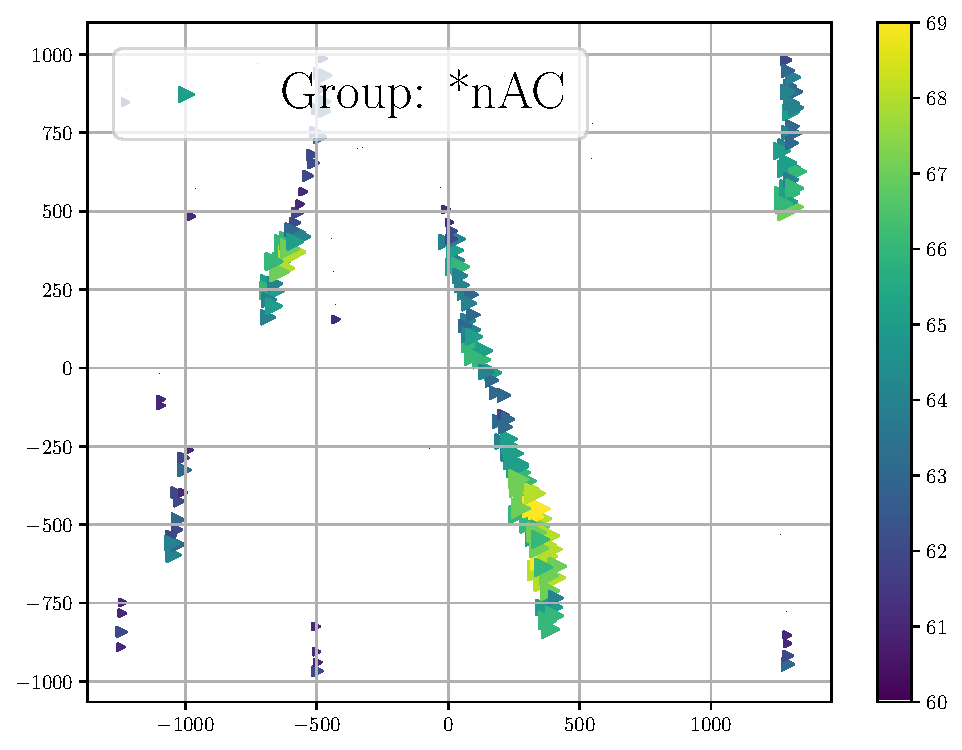
\includegraphics[width=.4\textwidth]{Img/chapter10/PI-Class-group-sample5.pdf}
%\includegraphics[width=.4\textwidth]{Img/chapter10/Class-align-sample4.pdf}
%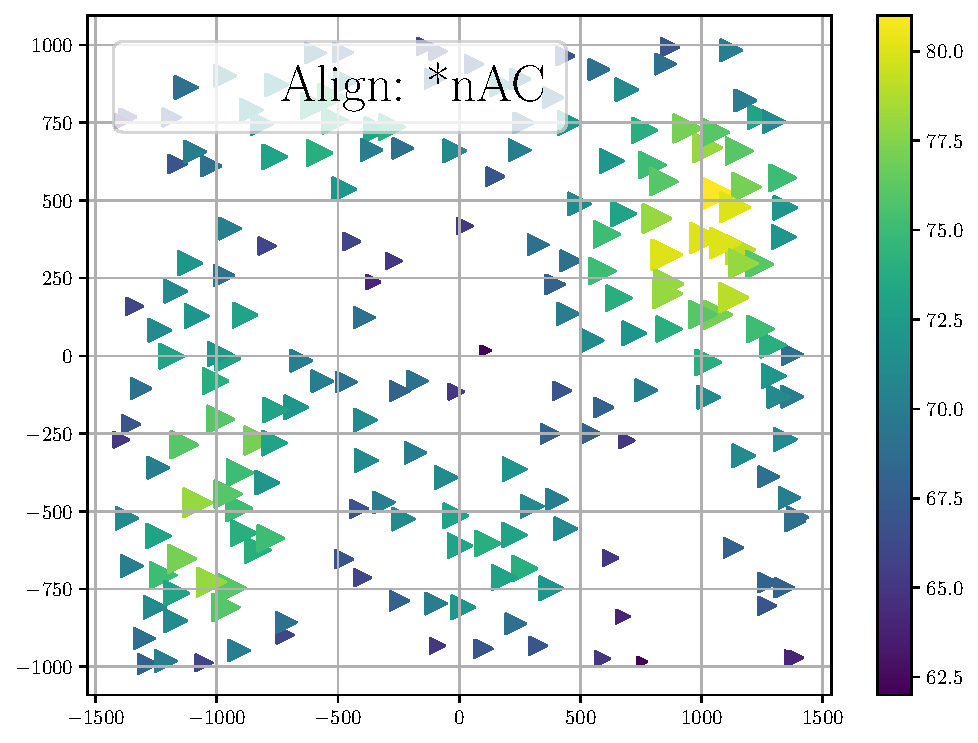
\includegraphics[width=.4\textwidth]{Img/chapter10/PI-Class-align-sample4.pdf}
%\caption{智能体合作关系的整体描述示意图}
%\label{fig:nAC-demon}
%\end{figure}

\begin{figure}
     \centering
     \begin{subfigure}[b]{.45\textwidth}
         \centering
         \includegraphics[width=1\textwidth]{Img/chapter10/Class-group-sample5.pdf}   
         \caption{无人机集群Group行为示意图}
         \label{group-sample5-coh}
     \end{subfigure}
     \hfill
     \begin{subfigure}[b]{.45\textwidth}
         \centering
         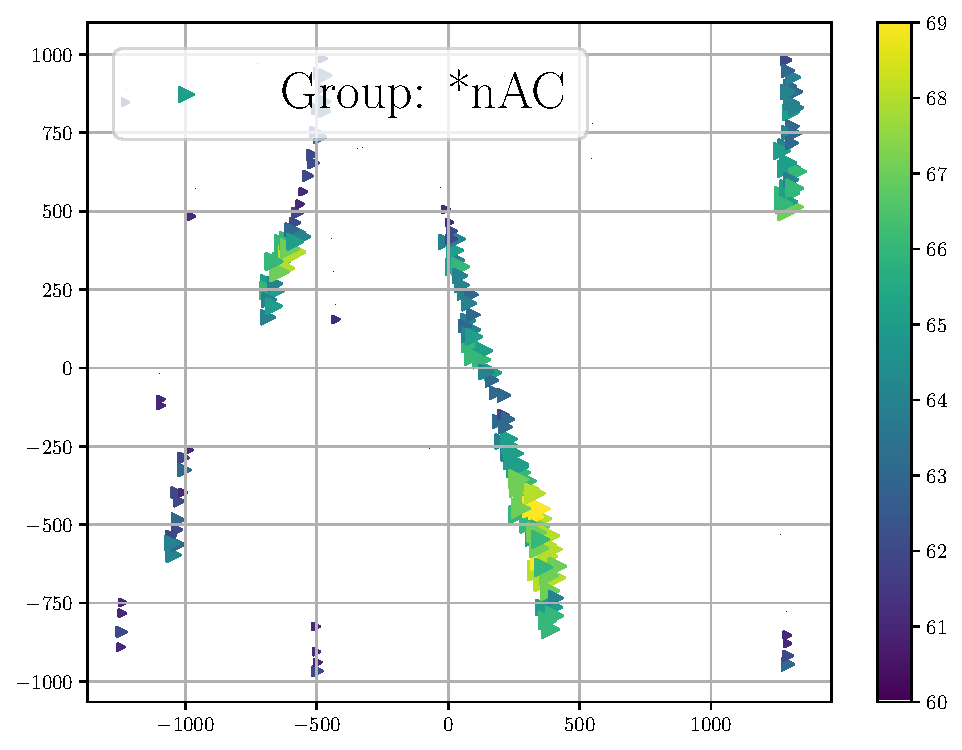
\includegraphics[width=1\textwidth]{Img/chapter10/PI-Class-group-sample5.pdf}
         \caption{Group行为对应合作关系描述示意图}
         \label{group-sample5-coh1}
     \end{subfigure}
     \hfill
     \begin{subfigure}[b]{.45\textwidth}
         \centering
         \includegraphics[width=1\textwidth]{Img/chapter10/Class-align-sample4.pdf}
         \caption{无人机集群Align行为示意图}
         \label{align-sample5-coh}
     \end{subfigure}
     \hfill
     \begin{subfigure}[b]{.45\textwidth}
         \centering
         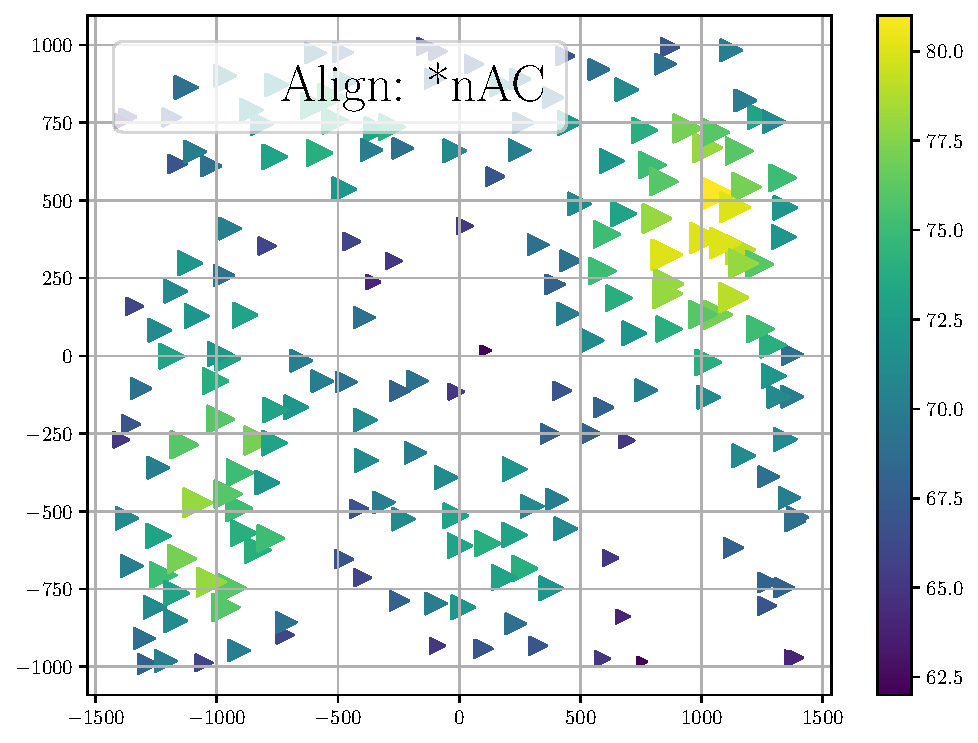
\includegraphics[width=1\textwidth]{Img/chapter10/PI-Class-align-sample4.pdf}
         \caption{Align行为对应合作关系描述示意图}
         \label{align-sample5-coh1}
     \end{subfigure}          
\caption{智能体合作关系的整体描述示意图}
\label{fig:nAC-demon}
\end{figure}

这就可以给一种启示, 如果将这类合作特权信息加入模型, 会不会能够增加学习的收敛速率。类似的结果也在 Align行为中得以展现, 图 \ref{align-sample5-coh} 的展示的是Align行为, 其对应的特权信息{Align: *nAC}为图\ref{align-sample5-coh1}。 从图中可以直观地看到类似的结果, 即对于Align行为, 特权信息{Align: *nAC}在智能体聚集的区域取值较高, 在智能体分散的区域取值较低。 因此, 希望这种对智能体直观的整体描述能够加速集群行为识别的收敛速率。

另外, 还提出另一种整体性描述智能体的特权信息。 将处在Separation向量半径内的智能体数目视作是竞争描述。 从介绍无人机集群行为数据集的描述中可知, Separation向量刻画的是智能体彼此之间处于分离状态的向量, 因此, 在Separation向量半径内的智能体数目直观上可以视为是一种竞争关系的尺度。图\ref{fig:nS-demon} 展示两种集群行为下所对应的竞争关系。 图 \ref{group-sample5-jz} 展示的是Group行为, 此时其对应的特权信息是图\ref{group-sample5-jz1}。 特权信息{Group:*nS}图中采用热力图标示{nS}数目的大小区别, 从图中可以看到, 智能体聚集的部分其特权信息{Group: *nS}的取值较高, 智能体分散的部分其特权信息{Group: *nS}的取值较低。 

%
%\begin{figure}
%\centering
%\includegraphics[width=.4\textwidth]{Class-group-sample5.pdf}
%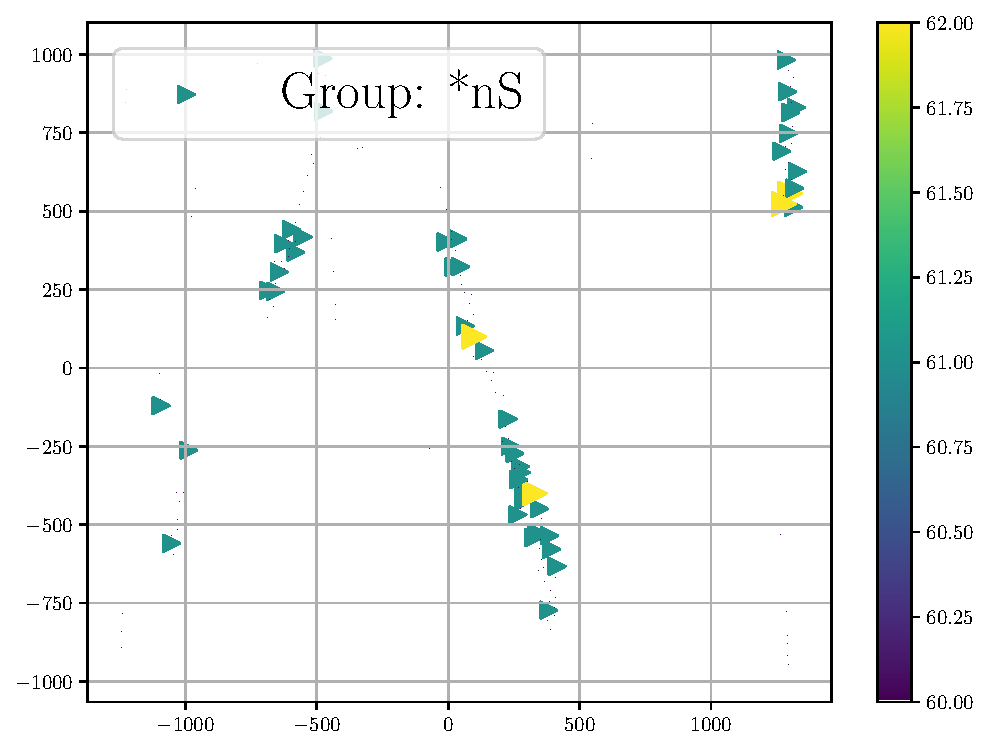
\includegraphics[width=.4\textwidth]{S-PI-Class-group-sample5.pdf}
%\includegraphics[width=.4\textwidth]{Class-align-sample4.pdf}
%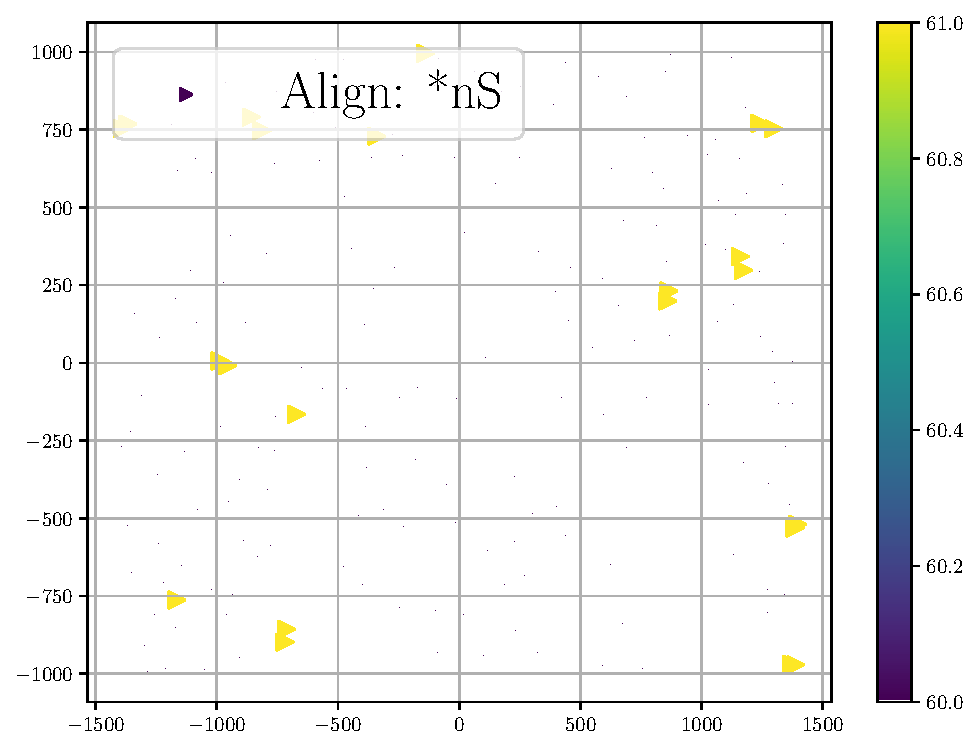
\includegraphics[width=.4\textwidth]{S-PI-Class-align-sample4.pdf}
%\caption{智能体竞争关系的整体描述示意图}
%\label{fig:nS-demon}
%\end{figure}

\begin{figure}
     \centering
     \begin{subfigure}[b]{.45\textwidth}
         \centering
         \includegraphics[width=1\textwidth]{Class-group-sample5.pdf}   
         \caption{无人机集群Group行为示意图}
         \label{group-sample5-jz}
     \end{subfigure}
     \hfill
     \begin{subfigure}[b]{.45\textwidth}
         \centering
         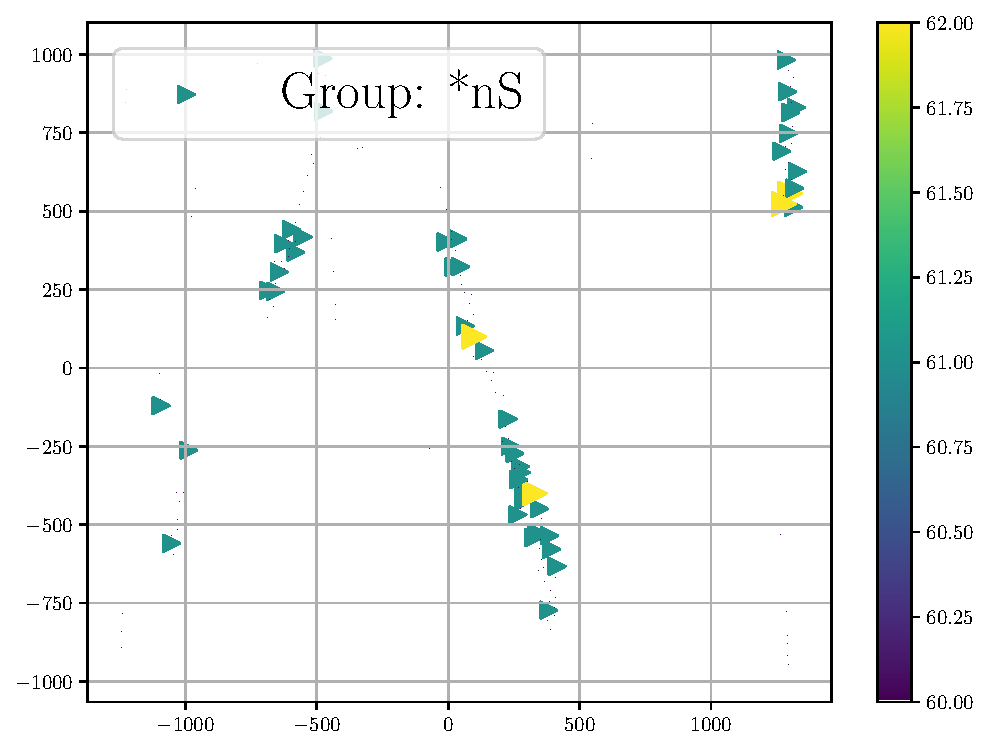
\includegraphics[width=1\textwidth]{S-PI-Class-group-sample5.pdf}
         \caption{Group行为对应竞争关系描述示意图}
         \label{group-sample5-jz1}
     \end{subfigure}
     \hfill
     \begin{subfigure}[b]{.45\textwidth}
         \centering
         \includegraphics[width=1\textwidth]{Class-align-sample4.pdf}
         \caption{无人机集群Align行为示意图}
         \label{align-sample5-jz}
     \end{subfigure}
     \hfill
     \begin{subfigure}[b]{.45\textwidth}
         \centering
         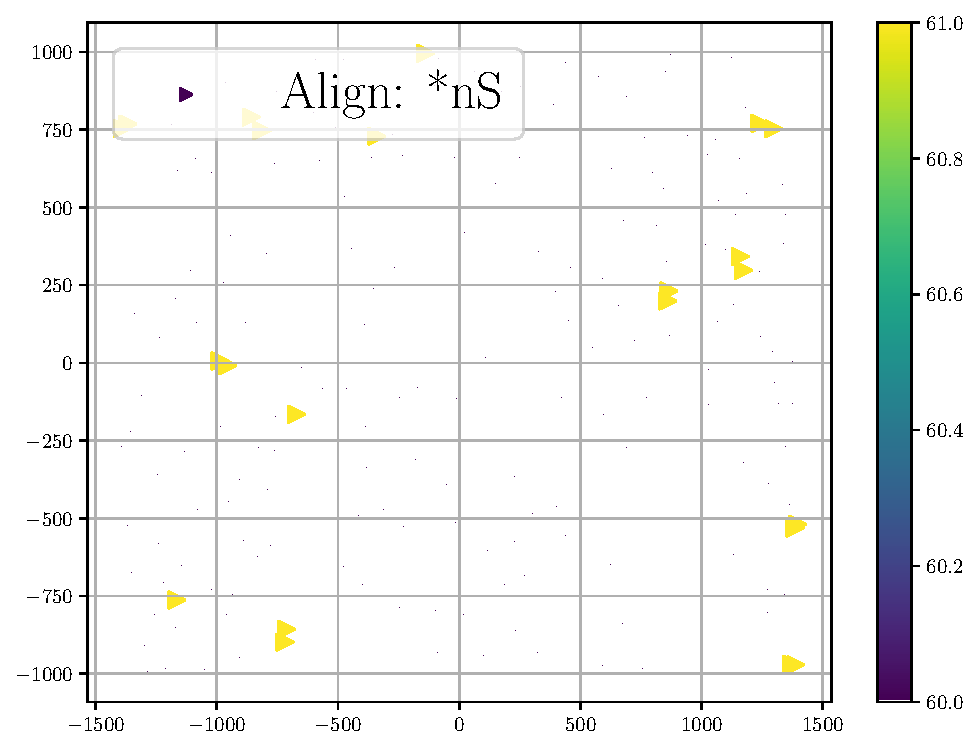
\includegraphics[width=1\textwidth]{S-PI-Class-align-sample4.pdf}
         \caption{Align行为对应竞争关系描述示意图}
         \label{align-sample5-jz1}
     \end{subfigure}          
\caption{智能体竞争关系的整体描述示意图}
\label{fig:nS-demon}
\end{figure}

同样地, 如果将这类反映智能体“竞争激烈”的特权信息加入模型, 会不会能够增加学习的收敛速率。 类似的结果也在 Align行为中得以展现, 图 \ref{align-sample5-jz} 展示的是Align行为, 其对应的特权信息{Align: *nS}为图\ref{align-sample5-jz1} 所示。整体上而言, 特权信息{Align: *nS}在智能体聚集的区域取值较高, 在智能体分散的区域取值较低。 这些取值高低的分布可以朴素地理解为智能体之间“竞争”的激烈程度的度量。因此, 希望这种对智能体直观的竞争描述也能够加速集群行为识别的收敛速率。

对于特权学习建模, 考虑两种建模方法, 
\begin{enumerate}
\item[1.] 一般通用LUPI算法 (LUPI-X*): 在这种模型中, 特权空间直接由核函数 $K^{*}(x_{i}^{*},x_{j}^{*})$定义。
\item[2.] 特定具体LUPI算法 (LUPI-d): 在这种模型中, 特权空间是由具体的一维 $d$-空间所定义的, 此$d$-空间是由SVMs按照下列步骤实施的, 即
\begin{enumerate}
\item[(1)] 首先, 给定下列数据对
\begin{align}
(x_{1}^{*}, y_{1}), \ldots, (x_{l}^{*},y_{l}).
\end{align}
考虑在空间 $X^{*}$中寻找一个决策规则, 然后提取此问题的得分函数 $\hat{y}_{i}$。
\item[(2)] 使用在空间$X^{*}$中的得分函数来定义下列偏差值 $d_{i} = 1-y_{i}\hat{y}_{i}$。
\item[(3)] 使用下列三元组构建LUPI模型
\begin{align}
(x_{1}, d_{1}, y_{1}), \ldots, (x_{l}, d_{1}, y_{l}).
\end{align}
\end{enumerate} 
\end{enumerate}

在下一章节将展示一般通用LUPI算法和特定具体LUPI算法在集群行为数据集上的结果。

\section{整体描述作为特权信息加速分类算法收敛研究}

本节介绍两种针对无人机集群行为的整体描述作为特权信息, 加速LUPI算法收敛。第一种整体描述信息提供了针对无人机集群的合作描述; 第二种整体描述信息提供了针对无人机集群的竞争描述。

\subsection{无人机集群的合作描述作为特权信息}
本节针对合作描述作为特权信息的LUPI方案设计展开研究。提出诸智能体之间彼此如何“合作”的整体描述作为特权信息来验证LUPI方法的有效性和优势。 按照集群行为数据的原始顺序将数据切分为两部分: 使用前100个数据作为训练集, 后面10000个数据用于测试集, 重复试验20次取平均值。 这里需要专门指出, 确实是采用小量样本训练而测试大样本。 

考虑四种不同的机器学习算法进行对比, 分别是经典SVMs算法, 神经网络算法, LUPI-X*算法和LUPI-d算法。四种算法都采取默认参数, 即在SVMs中采用RBF核函数, 容量因子C=1; 在神经网络算法中采用默认参数, LUPI中决策空间采用RBF核函数, 特权空间采用线性核函数。 这四种算法分别在三种集群行为数据集上训练。 表\ref{tab:PI-nAC-LUPI-X}和表\ref{tab:PI-nAC-LUPI-d}分别列出了合作关系作为特权信息的LUPI-X*方法和LUPI-d方法分类准确度对比表。

具体而言, 对于表\ref{tab:PI-nAC-LUPI-X}中的Align数据集, 标准的SVMs算法和神经网络算法分别获得 74.54\% 和 48.57\% 的分类准确度, LUPI-X*方法将之提升至 82.31\%, 提升幅度分别为10.42\%和69.47\%; 对于Flock数据集, 标准的SVMs算法和神经网络算法分别获得 50.59\% 和 59.26\% 的分类准确度, LUPI-X*方法将之提升至 60.65\%, 提升幅度分别为19.04\%和2.35\%; 对于Group数据集, 标准的SVMs算法和神经网络算法分别获得 59.24\% 和 44.36\% 的分类准确度, LUPI-X*方法将之提升至 64.45\%, 提升幅度分别为9.79\%和45.29\%。

对于LUPI-d算法, 如表\ref{tab:PI-nAC-LUPI-d}结果所示, 对于Align数据集, 标准的SVMs算法和神经网络算法分别获得 74.54\% 和 48.57\% 的分类准确度, LUPI-d方法将之提升至 82.31\%, 提升幅度分别为10.42\%和69.47\%; 对于Flock数据集, 标准的SVMs算法和神经网络算法分别获得 50.59\% 和 59.26\% 的分类准确度, LUPI-d方法将之提升至 66.79\%, 提升幅度分别为31.09\%和12.71\%; 对于Group数据集, 标准的SVMs算法和神经网络算法分别获得 59.24\% 和 44.36\% 的分类准确度, LUPI-d方法将之提升至 73.55\%, 提升幅度分别为24.16\%和65.80\%。

\begin{table}[]
\centering
\caption{合作关系作为特权信息的LUPI-X*方法分类准确度对比表}
\label{tab:PI-nAC-LUPI-X}
\begin{tabular}{cccccc}
\hline
      & SVMs   & \begin{tabular}[c]{@{}c@{}}神经 \\ 网络\end{tabular} & LUPI-X* & \begin{tabular}[c]{@{}c@{}}LUPI-X*较SVMs\\ 提升百分比\end{tabular} & \begin{tabular}[c]{@{}c@{}}LUPI-X*较NN\\ 提升百分比\end{tabular} \\ \hline
Align & 74.54 & 48.57                                                      & \textbf{82.31}   & 10.42\%                                                     & 69.47\%                                                    \\
Flock & 50.95 & 59.26                                                      & \textbf{60.65}   & 19.04\%                                                     & 2.35\%                                                     \\
Group & 59.24 & 44.36                                                      & \textbf{64.45}   & 9.79\%                                                      & 45.29\%                                                    \\ \hline
\end{tabular}%
\end{table}

% Please add the following required packages to your document preamble:
% \usepackage{graphicx}
\begin{table}[]
\centering
\caption{合作关系作为特权信息的LUPI-d方法分类准确度对比表}
\label{tab:PI-nAC-LUPI-d}
\begin{tabular}{cccccc}
\hline
      & SVMs   & \begin{tabular}[c]{@{}c@{}}神经 \\ 网络\end{tabular} & LUPI-d & \begin{tabular}[c]{@{}c@{}}LUPI-d较SVMs\\ 提升百分比\end{tabular} & \begin{tabular}[c]{@{}c@{}}LUPI-d较NN\\ 提升百分比\end{tabular} \\ \hline
Align & 74.54 & 48.57                                                      & \textbf{82.31}  & 10.42\%                                                    & 69.47\%                                                   \\
Flock & 50.95 & 59.26                                                      & \textbf{66.79}  & 31.09\%                                                    & 12.71\%                                                   \\
Group & 59.24 & 44.36                                                      & \textbf{73.55}  & 24.16\%                                                    & 65.80\%                                                   \\ \hline
\end{tabular}%
\end{table}


以上结果表明, 通过考量在训练阶段可用但是无法在测试阶段采用的有关无人机集群整体合作关系的描述, 基于LUPI方法能够提升模型的学习推广能力。 同时这些试验表明, 特定具体LUPI算法(即LUPI-d方法)的学习推广能力最优, 这也能够支持\citet{Vapnik-similary-2015,vapnik2015}提出的知识转换的结果。

众所周知, 无人机集群研究中智能体数目会影响智能体彼此之间的合作关系。直观而言, 智能体数目越多, 合作关系越突出, LUPI算法中引进的特权信息对模型的贡献度应该越明显。 因此在不同的算法下考察智能体数目对分类准确度的影响, 对比智能体数目从10至100之间, 不同算法的预测准确度。

图 \ref{fig:agents-accuracy} 给出SVMs算法、神经网络算法和LUPI-d算法三种算法的预测结果。 从图中可以看到标准SVMs算法作为基准算法, 其预测性能表现保持稳定。对于神经网络算法采用默认全连接参数, 因为没有进行参数优化, 所以全连接神经网络算法的预测表现并不稳定。考虑整体描述信息的LUPI算法随着智能体数目增加到一定规模后, 其预测能力稳步提升, 并且整体上均由于其他两种算法。 

\begin{figure}
\centering
\includegraphics[width=.7\textwidth]{Img/chapter10/align-agent-PI1.pdf}
\includegraphics[width=.7\textwidth]{Img/chapter10/flock-agent-PI1.pdf}
\includegraphics[width=.7\textwidth]{Img/chapter10/group-agent-PI1.pdf}
\caption{合作关系作为特权信息的LUPI方法分类准确度比较}
\label{fig:agents-accuracy}
\end{figure}

具体而言, 对于Align数据集 (图\ref{fig:agents-accuracy}上图)SVMs算法的预测准确率集中在0.7454; 神经网络算法受集群智能体个数的影响波动比较大, 并且总体而言其学习推广能力相较于SVMs算法和LUPI算法都较差; LUPI算法在当智能体数目小于30时, 学习推广能力波动较大, 但是当智能体数目大于30之后, LUPI算法的学习推广能力明显优于SVMs算法和神经网络算法。对于Flock数据集 (图\ref{fig:agents-accuracy}中图), SVMs算法预测性能并不会随着智能体数目的变化发生很大的波动, 而神经网络算法同样表现出比较大的波动, LUPI算法则明显优于另外两种算法。 最后, 相同的结果也适用于Group数据集 (图\ref{fig:agents-accuracy}下图), 即SVMs算法能够得到相对稳定的结果, 神经网络算法受智能体数目增加的影响会产生较大的波动, 并且大多数情形下其学习推广能力都表现的不尽人意 (因为都采取的是默认参数, 此时的神经网络未经过参数寻优), 而LUPI算法则随着智能体数目的增加, 其学习推广能力会稳定地优于另两种现代机器学习算法。


\subsection{无人机集群的竞争描述作为特权信息}
对于仿生集群行为分类问题, 与之前所述的合作关系类似, 考虑智能体彼此之间的竞争关系。 对于仿生集群行为, Separation向量描述智能体彼此之间的分离关系, 因此直观上而言, 可以借用每个智能体处在Separation向量半径内的数目来刻画智能体彼此之间的“竞争关系”。还是按照数据集原初顺序将集群数据集分为训练集和测试集并且择使用150个训练样本预测后面10000个数据。

表 \ref{tab:sample-error-LUPI-X} 和表 \ref{tab:sample-error-LUPI-d} 列出将竞争描述作为特权信息的LUPI方法在此实验下利用四种学习算法的分类准确率, 这两个表中所得结果是相同的。 其中, 四种算法都采取默认参数, 即在SVMs中采用RBF核函数, 容量因子C=1; 在神经网络算法中采用默认参数, LUPI中决策空间采用RBF核函数, 特权空间采用线性核函数。 这四种算法分别在三种集群行为数据集上训练, 从表\ref{tab:sample-error-LUPI-X} 和表 \ref{tab:sample-error-LUPI-d}可以看到, 对于Align行为数据集, LUPI-X*算法和LUPI-d算法比常规SVMs算法提升13.70\%, 而对神经网络算法则提升高达143.96\%; 对于Flock行为数据集, LUPI-X*算法和LUPI-d算法比常规SVMs算法提升20.63\%, 而对神经网络算法则提升高达68.75\%; 对于Group行为数据集, LUPI-X*算法和LUPI-d算法比常规SVMs算法提升11.14\%, 但对神经网络算法则没有提升, 但是两者预测效果相差不大。


\begin{table}[]
\centering
\caption{竞争关系作为特权信息的LUPI-X*方法分类准确度对比表}
\label{tab:sample-error-LUPI-X}
\begin{tabular}{cccccc}
\hline
      & SVMs   & \begin{tabular}[c]{@{}c@{}}神经 \\ 网络\end{tabular} & LUPI-X* & \begin{tabular}[c]{@{}c@{}}LUPI-X*较SVMs\\ 提升百分比\end{tabular} & \begin{tabular}[c]{@{}c@{}}LUPI-X*较NN\\ 提升百分比\end{tabular} \\ \hline
Align & 74.54 & 37.74                                                      & \textbf{84.75}   & 13.70\%                                                     & 143.96\%                                                   \\
Flock & 50.85 & 36.35                                                      & \textbf{61.34}   & 20.63\%                                                     & 68.75\%                                                    \\
Group & 59.27 & \textbf{66.41}                                                      & 65.87   & 11.14\%                                                     & -0.81\%                                                    \\ \hline
\end{tabular}%
\end{table}

\begin{table}[]
\centering
\caption{竞争关系作为特权信息的LUPI-d方法分类准确度对比表}
\label{tab:sample-error-LUPI-d}
\begin{tabular}{cccccc}
\hline
      & SVMs   & \begin{tabular}[c]{@{}c@{}}神经 \\ 网络\end{tabular} & LUPI-d & \begin{tabular}[c]{@{}c@{}}LUPI-d较SVMs\\ 提升百分比\end{tabular} & \begin{tabular}[c]{@{}c@{}}LUPI-d较NN\\ 提升百分比\end{tabular} \\ \hline
Align & 74.54 & 37.74                                                      & \textbf{84.75}   & 13.70\%                                                     & 143.96\%                                                   \\
Flock & 50.85 & 36.35                                                      & \textbf{61.34}   & 20.63\%                                                     & 68.75\%                                                    \\
Group & 59.27 & \textbf{66.41}                                                      & 65.87   & 11.14\%                                                     & -0.81\%                                                    \\ \hline
\end{tabular}%
\end{table}


具体而言, 对于Align数据集, LUPI系列算法比标准SVMs算法和神经网络算法都优异; 标准的SVMs算法和神经网络算法分别获得 74.54\% 和 37.74\% 的分类准确度, 而LUPI方法将之提升至 84.75 \%; 对于Flock数据集, 标准的SVMs算法和神经网络算法分别获得 50.85\% 和 36.35\% 的分类准确度, LUPI系列方法将之提升至 61.34 \%分类准确度; 而对于Group数据集, 标准的SVMs算法和神经网络算法分别获得 59.27\% 和 66.41\% 的分类准确度, LUPI系列方法分别获得 65.87\% 的分类准确度, 稍微低于最优的神经网络算法。 这些结果都表明, 通过考量在训练阶段可用但是无法在测试阶段采用的有关无人机集群的整体竞争关系描述, LUPI方法能够提升模型的学习推广能力。 

同时, 讨论训练样本数目与收敛速率的关系。直观上而言, 随着样本数目增多算法更容易收敛。而根据VC理论可知LUPI算法有可能实现小样本下高精度预测, 即LUPI算法有可能不需要太多样本就可以实现高精度预测。因此, 考察随着样本数目的增加各个模型错误分类的变化关系。 图 \ref{fig:sample-error} 展示针对三种集群行为数据集, 当训练样本量从50增加至150时, 三种机器学习分类错误率的变化情况。 从图中可以看到, 总体而言LUPI方法能够保持最佳的学习推广能力, 其受样本量增加的影响比较小, 基本能够保持稳定的分类错误率, 特别是在小量样本下仍然能够获得最低的错误分类。 

\begin{figure}
\centering
\includegraphics[width=.7\textwidth]{Img/chapter10/align-sample-PI2.pdf}
\includegraphics[width=.7\textwidth]{Img/chapter10/flock-sample-PI2.pdf}
\includegraphics[width=.7\textwidth]{Img/chapter10/group-sample-PI2.pdf}
\caption{竞争关系作为特权信息的LUPI方法分类错误率比较}
\label{fig:sample-error}
\end{figure}


具体而言, 对于Align数据集 (图\ref{fig:sample-error}上图), 当样本小于60时, SVMs方法表现出最低的推广泛化能力, 其对应的分类错误率最高; 当样本数目大于60后, SVMs方法和LUPI方法预测效果趋于稳定, 并且LUPI方法的预测效果比SVMs方法要优异。 但是对于神经网络算法, 由于并没有进行网络参数优化, 所以导致神经网络算法的预测性能受训练样本数目改变的影响较大。 对于Flock数据集(图\ref{fig:sample-error}中图)和Group数据集 (图\ref{fig:sample-error}下图), LUPI算法也依然保持稳健且优异的预测能力, 另两种算法的表现与Align数据集保持类似的结果。 

这样的结果也符合的预期, 正如VC理论所指明的, 通过引进特权信息, LUPI算法确实可以加速学习模型的收敛速率 (在这三个数据集上, 完全可以只采用50个样本就可以达到比标准SVMs算法、神经网络算法更好的预测效果)。 这样的结果是不奇怪的, 因为借助LUPI算法能够对集群行为提供整体的描述, 这样就使得学习算法能够加速收敛速率。

  
\section{本章小结}
\label{sec:discuss}
本节为无人机集群行为分类提供一种使用特权信息学习(Learning Using Privileged Information, LUPI)的新方法, 这种学习方法通过融合在训练阶段可用但是在测试阶段不可用的信息(此信息称为“特权信息”)来加速学习算法的收敛速度。主要结论总结如下:
\begin{enumerate}
\item 研究针对无人机集群行为整体描述的合作关系作为特权信息时LUPI算法的效果。研究结果表明, LUPI方法能够显著提升算法预测精度, 在三种无人机集群行为数据集上较基准SVMs算法提升分别为10.42\%, 31.09\% 和 24.16\%;
\item 研究针对无人机集群行为整体描述的竞争关系作为特权信息时LUPI算法的效果。研究结果表明, LUPI方法大都能够提升算法预测精度, 在三种无人机集群行为数据集上较基准SVMs算法提升分别为13.70\%, 20.63\% 和 11.14\%;
\item 比较智能体数目与无人机集群合作关系的影响, 以及无人机集群训练样本数目与LUPI算法收敛速度的影响。研究结果表明, 采用LUPI算法能够提升学习算法的收敛速度, 实现在无人机集群行为分类任务中小样本高精度预测的目标。
\end{enumerate}

\chapter{总结与展望}
\label{chapter:conclusion}

\section{论文工作总结}

鉴于复杂无人机集群行为通常和无人机集群任务分配具有强关联性, 本文基于无人机集群位置信息, 借助机器学习算法反演无人机集群行为, 并结合实际工程中无人机集群行为分类问题特点, 开展了四个方面的研究, 主要工作总结如下:

\begin{enumerate}
\item 研究无人机集群行为分类不确定量化方法。

提出一种使用一致性预测框架为无人机集群行为分类提供不确定量化研究解决方案。一致性预测方法提供两种预测模式, 其一, 置信预测, 此模式为机器学习算法输出提供一种无分布假设的不确定量化方法。 其二, 集合预测, 此模式为复杂无人机行为提供多类别的集合映射模式。试验结果表明, 所提方法可以为机器学习算法提供有效统计推断, 为解决复杂无人机集群行为分类问题中不确定量化研究提供一种解决方案。
\item 研究无人机集群行为数据本身的分布漂移检测。

提出一种使用鞅序列方法来实现针对无人机集群行为数据本身的分布漂移检测问题。 所提方法可建立在机器学习算法之上, 仅需要比较鞅序列最终值是否大于给定阈值就可以判定数据是否发生分布漂移, 为高维复杂无人机集群数据的分布漂移检测难题提出一种求解方法。试验结果表明, 所提方法能够实现对无人机集群行为数据分布漂移检测提供端到端的高效解决方案。
\item 研究使用鞅保护分布方法来改进底层机器学习算法的预测性能。

提出一种使用鞅保护分布算法(此方法融合了分布漂移信息)来增强底层分类算法的预测能力。 将基于鞅序列分布漂移检测理论和机器学习算法相结合, 改进常规机器学习算法预测性能。试验结果表明, 提出的鞅保护分布算法对大多数机器学习模型都有明显提升效果。
\item 研究小样本下高精度无人机集群行为分类方法。

提出一种使用特权信息学习范式实现小样本下高精度预测的方法。将无人机集群的整体描述作为特权信息纳入机器学习模型, 使得在小样本下达到高精度预测的目标。试验结果表明, 使用特权信息学习模型能够明显提升学习算法收敛速度, 使无人机集群行为分类在小样本下也可以达到较高精度的预测效果。
\end{enumerate}

\section{论文创新点}

本论文主要创新点如下:

\begin{enumerate}
\item 针对无人机集群行为分类, 提出采用一致性预测框架为机器学习算法输出结果提供不确定量化。应用蒙德里安一致性预测实现无人机集群行为分类不确定量化结果, 给出置信预测和集合预测两种不确定量化解决方案。
\item 针对实际工程应用需考虑数据本身分布的要求, 提出无分布假设的分布漂移检测方案。设计考虑数据本身分布信息的鞅保护分布算法, 改进底层机器学习算法预测性能, 为无人机集群行为分类问题提供一种新的高精度预测解决方案。
\item 提出使用特权信息模型加速分类算法收敛速度。设计针对无人机集群行为的两种整体描述信息, 验证整体描述作为特权信息的有效性, 实现小样本高精度无人机集群行为分类目标。
\end{enumerate}

\section{论文工作展望}

在本文已有研究工作基础上, 下一步工作可在以下几个方面展开:

\begin{enumerate}
\item 一致性预测框架为机器学习算法提供不确定量化的研究中, 可信度的效率与选取的非一致性得分函数有关。因此, 后续研究可以考虑如何提供更加高效的非一致性度量函数。
\item 无分布假设的鞅序列分布漂移检测研究中, 鞅理论提供的拒绝零假设证据建立在底层算法基础之上, 是一种依概率收敛的应诺式结果。因此, 后续研究可以探究如何改进底层学习算法。
\item 使用特权信息学习模型研究中, 模型预测效果与研究者提供的整体描述信息密切关联。因此, 后续研究可以探讨如何提供具有“先入之见”的特权信息, 以减少人工试错成本。
\end{enumerate}
%---------------------------------------------------------------------------%
% main content
%-
%-> Appendix
%-
\cleardoublepage%
%\appendix% initialize the environment
%\input{Tex/Appendix}% appendix content
%-
%-> Backmatter: bibliography, glossary, index
%-
\backmatter% initialize the environment
\intotoc*{\cleardoublepage}{\bibname}% add link to toc
\artxifstreq{\artxbib}{bibtex}{% enable bibtex
    \bibliography{Biblio/ref}% bibliography
}{%
    \printbibliography% bibliography
}
%---------------------------------------------------------------------------%
%->> Backmatter
%---------------------------------------------------------------------------%
\chapter[致谢]{致\quad 谢}\chaptermark{致\quad 谢}% syntax: \chapter[目录]{标题}\chaptermark{页眉}
%\thispagestyle{noheaderstyle}% 如果需要移除当前页的页眉
%\pagestyle{noheaderstyle}% 如果需要移除整章的页眉

回首求学历程,感慨颇多。在本文完成之际,作者谨向给予我指导、关心、支持、帮助和点拨我的老师、同学和亲人们致以衷心的感谢!

首先, 我要衷心地特别感谢我的导师陈洪波教授。 毫无疑问此论文它的前提始终无法离开我的导师陈洪波教授的支持。 我要特别感谢陈教授为我在攻博期间的科研工作提供了极具优越的平台和条件; 我要特别感谢陈老师在攻博开题阶段以及在北京联培期间为我的研究给予的关切和指导; 更重要的是, 特别感恩陈老师对于团队以及我个人的教诲都始终站在国家、时代、人民的高度。 这样的言说还不仅仅只是停留在感激和感恩的层面, 更重要的恰恰是由于陈老师的点拨和教诲让我真切的意识到我们必须要在思想的事业上有最起码的路标, 而此路标的建构就无论如何都离不开这四年期间陈老师给我的指导和点拨。 

同时, 这篇论文得以可能的前提也与我在北京联合培养期间的导师陈小前研究员和姚雯研究员的支持密不可分。 感谢姚老师。 姚老师提供了极具前沿的课题, 本论文应用研究部分大都是在姚老师的课题下展开的, 并且也是在此课题的探索中启发了我必须批判地直面技术本身。 诚恳说来, 这样的课题要求已经在逻辑上规定了我本人进一步追问学习问题的一些方向。

感谢庄学彬副教授。 我攻博期间学术的开端是庄学彬老师提供的, 庄老师提供的前沿科研项目为我的研究提供了重要的应用背景并且开阔了学术眼界。 在庄老师的指导下我也能有机会深入理解一些课题方向并且有机会进入科研项目的语言体系中去。

感谢国防科技大学郭得科教授对我本人的关心和鼓励, 感谢郭老师在军科期间专门问询我本人的情况。感谢张英朝教授在我科研初期给予的点拨和鼓励。感谢国防科技大学任棒棒博士给我提供的帮助。

感谢兰州大学李周平老师提示我进入一致性预测研究领域,感谢李老师在我攻博期间对我特别的关怀和问询。感谢兰州大学李宪越老师给予我的提携和帮助, 有幸和李老师相识是我的福气。

我要特别感谢Vladimir Vapnik教授和Vladimir Vovk教授。 感谢Vladimir Vapnik教授在统计学习理论上给我额外重要的点拨。 感谢 Vladimir Vovk教授对我的鼓励。 正如Vladimir Vapnik教授所言, VC理论是思想的事业, 而思是我们这个时代的当务之急。我是在颇为不安地反思如何真切地辨明统计学与机器学习——最初是基于神经网络相关的机器学习——这两种知识类型的本质区别而展开研究。在学习理论中如何找出那条“林中路”是我一直以来在追问但又迟迟没解决的问题。 我一直是在统计学的框架下展开可信学习问题, 在这个框架下我研究的内容最后归结于如何获得有效的p-值。 直到2020年10月开始关注一致性预测方法, 因为这个方法能够自动保证p-值有效。 可以想见, 在先前那两三年的疑虑和困惑的停留中, 一致性预测方法为我开启了一种格外明朗的光照, 此光照起初在技术上的炫目让我深为服膺。 也正是在深入到一致性预测方法细节研究的时候——即如何理解非一致性得分函数——我真正开始阅读VC理论。 只有从存在论基础上深入地理解Vapnik统计学习理论哲学,不满足于当前主流受过逻辑训练心智给出的方案,关于学习理论的真正内容才有可能牵引着同我们真正照面。本文的第二章尝试着精要地给出这方面的一些结论。
%在我看来, Vapnik统计学习理论哲学唯有通过阅读Vapnik原著才能得以可能, 但是真正读懂Vapnik原著又需要读者自己发动革命。 这就给我们一个很有意思的循环: 要读懂Vapnik统计学习理论就需要Vapnik统计学革命思想, 而Vapnik统计学革命思想又在Vapnik统计学习理论中。 正就是在这样一种理解下我开始阅读Vapnik的原著, 通过阅读原著我的思想发生了彻底的转变。 Vapnik发动的统计学革命虽然在计算机领域的前沿研究中都得到了技术上的认可——这种认可更多由计算机领域的专家们以含蓄的技术阐述言说——但是在哲学的基础方面却并没有得到澄清, 甚至并未被真正研究过。 这里所说的基础方面最终涉及Vapnik统计学习理论哲学的存在论(ontology)根基。 如果这一根基本身依然停留在晦暗之中, 那么对于Vapnik统计学习理论的任何一种技术上的阐述就会是薄弱的和内在动摇的。 为了从先前知性的理解困境中摆脱出来, 我开始重新深入到VC理论的存在论基础上展开, 并对这一基础做出具有原则高度的阐释。 
%它的形式似乎基于统计学辩证法的, 的确我们需要给出统计学辩证法; 但真切的说来它的内容是存在论的, 是以重释VC理论存在论为枢轴的。 所以这就使得在内容上首先一定是批判的: 即不满足于当前主流受过逻辑训练心智给出的方案。 同时, 又是探索性的, 即试图在存在论的视域中来阐说VC理论。 

感谢在广州、北京学习期间遇到课题组的老师和同学的帮助, 感谢马才碑、马欣煜、王东华、王帅、王红亮、王超然、王晶、牛犇、左源老师、石涛、付鹏、包凯瑞、冯妤婕、朱效洲老师、刘书磊、刘旭、孙家亮、李桥、李超、肖叶、何雨昕、张云阳、张若凡、张泽雨、张晨、陈献琪博士、武领华、苗青、林子健、林煜龙、尚天赐、罗加享、郑小虎博士、项子雪、赵啸宇、姚炜杰、夏宇峰、唐贵建、彭兴文、曾小慧、曾昆、谢礼伟、谢扬帆、蔡鑫。

感谢南方科技大学的何帅达博士和兰州大学的刘倩倩博士提供的帮助和在前期展开关于统计学交流时提供的便捷。 感谢Wang Jie同学在关于存在论问题阐述时给出的积极反馈。

深深地感谢我的父亲和母亲。在我成长的每一个关键时期,都倾注了他们力所能及的最大支持。养儿方知父母恩。这样切近的体会,对语言所指和能指的真切把握是我自己成为父亲后方才领悟到的。

最后, 特别感谢爱人徐庆龄给予家庭的无尽付出。我唯有真切的进入真正的思以及勤勉的工作才是对家人默默支持最大的回报。 可以断言, 这也是家人所乐见的真正的自己。

\hfill \textit{席泽璞}

\hfill 2023年5月于广州中山大学


\chapter{作者攻读学位期间发表的学术论文与研究成果}
%
%\section*{作者简历:}
%
%席泽璞, 甘肃会宁人。 中山大学系统科学与工程博士研究生。 
%
%\begin{enumerate}
%\item[•] 2011年9月 - 2015年7月, 成都理工大学
%\item[•] 2015年9月 - 2018年7月, 兰州大学
%\item[•] 2019年9月 - 2023年7月, 中山大学
%\item[•] 2020年12月 - 2023年7月, 军事科学院国防科技创新研究院\quad 联合培养 
%\end{enumerate}

\section*{已发表文章}
\begin{enumerate}
\item 
\textbf{Zepu Xi}, Hongbo Chen, Xiaoqian Chen, Wen Yao. 
Conformal Prediction Enhanced SVMs for Swarm Behavior Classification. 
International Joint Conference on Neural Networks (IJCNN). 2023. (人工智能学术A类会议, CCF-C, 第一作者) 
\item 
\textbf{Zepu Xi}, Hongbo Chen, Xiaoqian Chen, Wen Yao. 
Swarm Behavior Recognition: Martingales Protected Paradigm. 
International Joint Conference on Neural Networks (IJCNN). 2023. (人工智能学术A类会议, CCF-C, 第一作者)
\item 
\textbf{Zepu Xi}, Hongbo Chen, Xiaoqian Chen, Wen Yao. 
Distributions-free Martingales Test Distributions-shift. 
International Neural Network Society Deep Learning Innovations and Applications Workshop (INNS DLIA 2023), 2023. (第一作者)
\item 
\textbf{Zepu Xi}, Xuebin Zhuang, Hongbo Chen. 
Conformal Prediction for Hypersonic Flight Vehicle Classification. 
Proceedings of Machine Learning Research (PMLR). 2022. (第一作者)
\item 
\textbf{Zepu Xi}, Hongbo Chen, Xiaoqian Chen, Wen Yao. 
Mondrian Conformal Prediction of Boosting for Swarm Behavior Recognition. 
2022 IEEE International Conference on Unmanned Systems ({IEEE ICUS}). 2022. (EI, 第一作者)
\item 
\textbf{Zepu Xi}. 
Distributions-free Martingale Test Distributions-shift for Swarm Behavior Prediction. 
IEEE WCCI 2022, 2022 International Joint Conference on Neural Networks (WCCI-IJCNN). 2022. (人工智能学术A类会议, CCF-C, 第一作者)
\item 
\textbf{Zepu Xi}, Xuebin Zhuang, Hongbo Chen. 
Post-selection Inference, with Application to Autoregressive Processes. 2021. 
International Conference on Mechanical, Aerospace and Automotive Engineering (CMAAE), 2021. (EI, 第一作者)
\item 
Kun Zeng, Xuebin Zhuang, Yangfan Xie, \textbf{Zepu Xi}. 
Hypersonic Vehicle Trajectory Classification Using Improved CNN-LSTM Model. 
2021 IEEE International Conference on Unmanned Systems (IEEE ICUS). 2021. (EI, 第四作者)
\item 
Yangfan Xie, Xuebin Zhuang, \textbf{Zepu Xi}, Hongbo Chen. 
Dual-Channel and Bidirectional Neural Network for Hypersonic Glide Vehicle Trajectory Prediction. 
IEEE Access, 2021. (SCI, 第三作者)
\end{enumerate}

%\section*{在学期间参加国际学术会议}
%\begin{enumerate}
%\item Conformal Prediction for Hypersonic Flight Vehicle Classification. 一致性和概率预测与应用大会(COPA2022). 主席: Vladimir Vovk. 英国, 布莱顿
%\item Distributions-free Martingale Test Distributions-shift for Swarm Behavior Prediction. IEEE计算智能学会(WCCI2022), 国际神经网络联合大会(IJCNN2022). 意大利, 帕多瓦
%\item Post-selection Inference, with Application to Autoregressive Processes. CMAAE2021. 中国香港
%\end{enumerate}

\section*{已投递文章}
\begin{enumerate}
\item 
\textbf{Zepu Xi}, Hongbo Chen, Xiaoqian Chen, Wen Yao. 
Online Inferring Swarm Behavior Using Privileged Information Learning. 
Engineering Applications of Artificial Intelligence (SCI, 在审, 第一作者)
\item 
\textbf{Zepu Xi}, Hongbo Chen, Xiaoqian Chen, Wen Yao. 
Comformal Prediction for Reliable Swarm Behavior Classification. 
Engineering Applications of Artificial Intelligence (SCI, 在审, 第一作者).
%\item \textbf{Zepu Xi}. Predicates Learning. (Submitted)
\end{enumerate}

%\section*{专利}
%\begin{enumerate}
%\item 庄学彬, 谢扬帆, 陈洪波, \textsf{席泽璞}, 曾昆. 一种基于双通道双向神经网络的飞行器轨迹预测方法[P]. 发明专利: CN112859898A, 2021-05-28. (已授权)
%\end{enumerate}
%
%
%
\section*{译著}
\begin{enumerate}
\item Vladimir N. Vapnik. 基于经验数据的相依关系估计[M]. 席泽璞, [译]. 第三版 (860+页), 2023. (第二次校稿中)
\end{enumerate}

\section*{参加的科研项目情况:}
\begin{enumerate}
\item 基于因果推断的XXX技术研究. 国防科技创新特区项目, 2022-2023年, 核心参与
\item 基于XXX技术研究. 国防科技创新研究院项目, 2021-2022年, 参与
\item 基于XXX信息的XXX预测技术研究. 国防科技创新特区项目, 2020-2021年, 核心参与
\item XXX系统韧性建模与评估研究. 装备预先研究项目, 2020-2021年, 核心参与
\end{enumerate}

\cleardoublepage[plain]% 让文档总是结束于偶数页,可根据需要设定页眉页脚样式,如 [noheaderstyle]
%---------------------------------------------------------------------------%
% other information
\end{document}
%---------------------------------------------------------------------------%

